\documentclass[12pt,a4paper,oneside, openany]{book}
\usepackage{lmodern}
\usepackage{setspace}
\setstretch{1.5}
\usepackage{amssymb,amsmath}
\usepackage{ifxetex,ifluatex}
\usepackage{fixltx2e} % provides \textsubscript
\ifnum 0\ifxetex 1\fi\ifluatex 1\fi=0 % if pdftex
  \usepackage[T1]{fontenc}
  \usepackage[utf8]{inputenc}
\else % if luatex or xelatex
  \ifxetex
    \usepackage{mathspec}
  \else
    \usepackage{fontspec}
  \fi
  \defaultfontfeatures{Ligatures=TeX,Scale=MatchLowercase}
\fi
% use upquote if available, for straight quotes in verbatim environments
\IfFileExists{upquote.sty}{\usepackage{upquote}}{}
% use microtype if available
\IfFileExists{microtype.sty}{%
\usepackage{microtype}
\UseMicrotypeSet[protrusion]{basicmath} % disable protrusion for tt fonts
}{}
\usepackage[left=3cm, right=2.5cm, top=3cm, bottom=2.5cm]{geometry}
\usepackage{hyperref}
\hypersetup{unicode=true,
            pdfborder={0 0 0},
            breaklinks=true}
\urlstyle{same}  % don't use monospace font for urls
\usepackage{longtable,booktabs}
\IfFileExists{parskip.sty}{%
\usepackage{parskip}
}{% else
\setlength{\parindent}{0pt}
\setlength{\parskip}{6pt plus 2pt minus 1pt}
}
\setlength{\emergencystretch}{3em}  % prevent overfull lines
\providecommand{\tightlist}{%
  \setlength{\itemsep}{0pt}\setlength{\parskip}{0pt}}
\setcounter{secnumdepth}{5}
% Redefines (sub)paragraphs to behave more like sections
\ifx\paragraph\undefined\else
\let\oldparagraph\paragraph
\renewcommand{\paragraph}[1]{\oldparagraph{#1}\mbox{}}
\fi
\ifx\subparagraph\undefined\else
\let\oldsubparagraph\subparagraph
\renewcommand{\subparagraph}[1]{\oldsubparagraph{#1}\mbox{}}
\fi

%%% Use protect on footnotes to avoid problems with footnotes in titles
\let\rmarkdownfootnote\footnote%
\def\footnote{\protect\rmarkdownfootnote}


  \title{}
    \author{}
    \date{}
  

\usepackage{booktabs}
\usepackage{longtable}
\usepackage[table]{xcolor}
\usepackage{array}
\usepackage{amsthm}
\usepackage{setspace}
\usepackage[nottoc]{tocbibind}
\usepackage[spanish]{babel}
\pagestyle{plain}
\raggedbottom
\usepackage{pdfpages}
\usepackage{float}
\usepackage{pdflscape}



\addto\captionsspanish{%
  \def\bibname{Referencias}%
  \def\tablename{Tabla}%
  \renewcommand{\listtablename}%
    {Índice de tablas}%
}

\usepackage{amsthm}
\newtheorem{theorem}{Theorem}[chapter]
\newtheorem{lemma}{Lemma}[chapter]
\theoremstyle{definition}
\newtheorem{definition}{Definition}[chapter]
\newtheorem{corollary}{Corollary}[chapter]
\newtheorem{proposition}{Proposition}[chapter]
\theoremstyle{definition}
\newtheorem{example}{Example}[chapter]
\theoremstyle{definition}
\newtheorem{exercise}{Exercise}[chapter]
\theoremstyle{remark}
\newtheorem*{remark}{Remark}
\newtheorem*{solution}{Solution}
\begin{document}
% 
\pagenumbering{gobble}
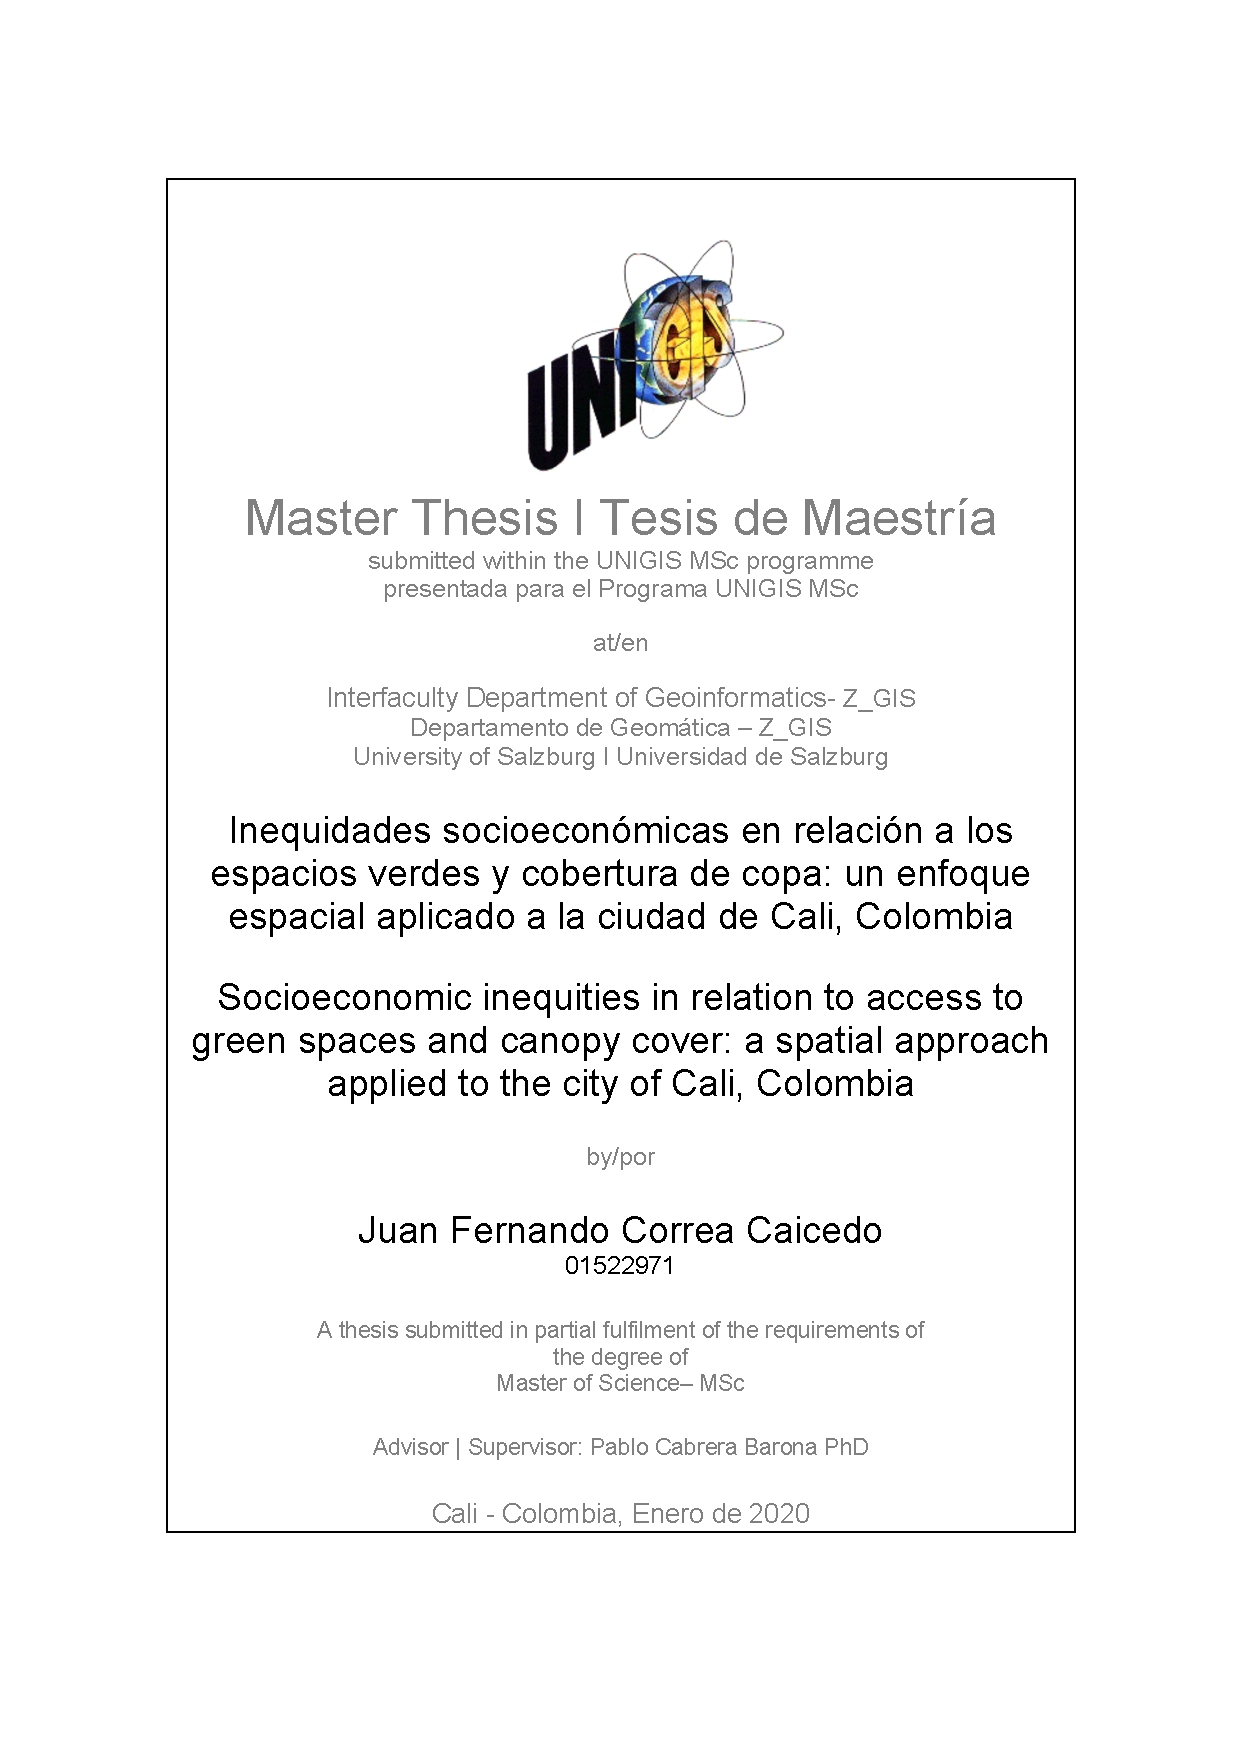
\includepdf[pages=1]{./incluir/Portada_oficial_Salzburg_2020.pdf}

\textbf{Compromiso de Ciencia}

Por medio del presente documento, incluyendo mi firma personal certifico
y aseguro que mi tesis es completamente el resultado de mi propio
trabajo. He citado todas las fuentes que he usado en mi tesis y en todos
los casos he indicado su origen.

\bigskip

Cali - Colombia, enero de 2020

\hrulefill 

Lugar, Fecha \hfill Firma

\chapter*{Agradecimientos}\label{agradecimientos}
\addcontentsline{toc}{chapter}{Agradecimientos}

A Elizabeth, por inculcarme la pasión por el conocimiento y las letras.
Augusto, por enseñarme la disciplina y valor del trabajo. Ana María, por
su solidaridad incondicional con mis proyectos. A Catalina, por su amor,
su compañía y paciencia con mi trabajo.

A Raul Sedano, Jeisson Ipia, Juan Felipe González y Anton Eitzinger por
su valiosos comentarios y realimentación a este trabajo.

A la gente del Internet, que generosamente comparte su conocimiento
convirtiéndolo en un espacio de aprendizaje y repositorio de saberes.

\setstretch{1.0}

\chapter*{Resumen}\label{resumen}
\addcontentsline{toc}{chapter}{Resumen}

\setstretch{1.0}

Esta investigación hace uso del censo arbóreo urbano realizado en
Santiago de Cali (Colombia) entre el año 2014 y 2015, de los datos del
censo de población de 2005 y los datos de la estructura ecológica del
municipio del 2014. El propósito es identificar si existen patrones
espaciales estadísticamente significativos que den evidencia de sesgos
de los indicadores de acceso a servicios ambientales del arbolado urbano
(AU) y espacios verdes (EV) con indicadores socioeconómicos, con el fin
de identificar espacialmente inequidades en el acceso a este tipo de
servicios ecosistémicos.

Para lograrlo se hace uso de modelos de regresión espacial que capturan
fenómenos de agrupamiento y dispersión en los patrones espaciales, a
través la inclusión de términos de autocorrelación espacial en la
regresión lineal. Los modelos espaciales de regresión se prueban con dos
tipos de matrices para observar el efecto de la topología de interacción
entre las variables y los resultados del ajuste. Se hace uso de gráficos
estadísticos, mapas temáticos y de LISA para la identificación de zonas
con concentración en el acceso.

Los resultados muestran que existen inequidades explicadas por variables
de estatus como el acceso a educación superior, que están además
negativamente correlacionadas con el porcentaje de afrocolombianos en un
sector censal urbano (SU). En relación al acceso a espacios verdes, no
existe evidencia fuerte de que las variable de etnicidad, salud o
estatus sean buenos predictores del acceso. Sin embargo, sí se encontró
una alta concentración del área del EV disponible en muy pocos sectores
de la ciudad.

\textbf{Palabras claves:} cobertura de copa, espacios verdes, justicia
ambiental, regresión espacial, servicios ambientales, indicadores
socioeconómicos.

\chapter*{Abstract}\label{abstract}
\addcontentsline{toc}{chapter}{Abstract}

\setstretch{1.0}

This study uses the urban arboreal census carried out in Santiago de
Cali (Colombia) between 2014 and 2015, the data of the 2005 population
census and the data of the ecological structure of the municipality of
2014. The purpose is to identify if there are spatially significant
patterns that provide evidence of biases in the indicators of access to
environmental services of urban trees (AU) and green spaces (EV) with
socioeconomic indicators, in order to spatially identify inequities in
access to these types of ecosystem services.

To achieve this, spatial regression models are used to capture grouping
and dispersion phenomena in spatial patterns through the inclusion of
terms of spatial autocorrelation in linear regression. The spatial
models are tested with two types of matrices to observe the effect of
the topology in the interaction between the variables and the results of
the adjustment. Statistical graphs, thematic and LISA maps are used to
identify areas with poor levels of access and discuss explanation
related to the causes.

The results show that there are inequities explained by status variables
such as access to higher education, which are also negatively correlated
with the percentage of Afro-Colombians in an urban census sector (SU).
In relation to access to green spaces (EV), there is no strong evidence
that the variables of ethnicity, health or status are good predictors of
access. However, there was a high concentration of the EV area available
in very few sectors of the city.

\textbf{Keywords:} canopy cover, green spaces, environmental justice,
spatial regression, environmental services, socioeconomic indicators.

\setstretch{1.5}

\setcounter{tocdepth}{2} \tableofcontents

\pagenumbering{arabic}

\chapter*{Glosario}\label{glosario}
\addcontentsline{toc}{chapter}{Glosario}

\begin{longtable}{>{\raggedright\arraybackslash}p{10cm}l}
\toprule
Término & Abreviación\\
\midrule
\endfirsthead
\multicolumn{2}{@{}l}{\textit{(continúa)}}\\
\toprule
Término & Abreviación\\
\midrule
\endhead
\
\endfoot
\bottomrule
\endlastfoot
\rowcolor{gray!6}  Criterio de información de Akaike o \textit{Akaike information criterion} & AIC\\
Arbolado Urbano & AU\\
\rowcolor{gray!6}  \textit{Cost-Benefit Analysis of Tree} & C-BAT\\
Censo Arbóreo de Cali 2015 & CA2015\\
\rowcolor{gray!6}  Monóxido de carbono & CO\\
\addlinespace
Censo de Población 2005 de Colombia & CP2005\\
\rowcolor{gray!6}  Corporación autónoma regional del Valle del Cauca & CVC\\
Departamento Administrativo de Gestión del Medio Ambiente & DAGMA\\
\rowcolor{gray!6}  Departamento Administrativo Nacional de Estadística & DANE\\
Estructura Ecológica Complementaria & EEC\\
\addlinespace
\rowcolor{gray!6}  Espacio Verde & EV\\
\textit{Geographically weighted regression} & GWR\\
\rowcolor{gray!6}  Infraestructura de Datos Espaciales de Santiago de Cali & IDESC\\
Lugares Especiales de Alojamiento & LEA\\
\rowcolor{gray!6}  \textit{Local indicators of spatial association} & LISA\\
\addlinespace
\textit{Maximum Likelihood} & ML\\
\rowcolor{gray!6}  Error cuadrático medio del inglés \textit{mean squared error} & MSE\\
\textit{Normalized difference vegetation index} & NDVI\\
\rowcolor{gray!6}  Dióxido de nitrógeno & NO$_2$\\
Ozono & O$_3$\\
\addlinespace
\rowcolor{gray!6}  \textit{Ordinary Least-Square} & OLS\\
Pequeñas partículas sólidas o líquidas dispersas en la atmósfera, y cuyo diámetro aerodinámico es menor que 10 $\mu$m & PM$_{10}$\\
\rowcolor{gray!6}  Plan de Ordenamiento Territorial & POT\\
Archipiélago de San Andrés, Providencia y Santa Catalina & SAI\\
\rowcolor{gray!6}  Modelo Autoregresivo o \textit{Spatial Autocorrelation} & SAR\\
\addlinespace
Modelo Espacial de Durbin & SD\\
\rowcolor{gray!6}  Modelo Espacial del Error o \textit{Spatial Error Model} & SEM\\
Retardo Espacial en X o \textit{Spatial Lag} & SLX\\
\rowcolor{gray!6}  Dióxido de azufre & SO$_2$\\
Sector Urbano & SU\\
\addlinespace
\rowcolor{gray!6}  \textit{Urban Forest Effects Model} & UFORE\\
\textit{Web Feature Service} & WFS\\*
\end{longtable}

\listoffigures

\listoftables

\chapter{Introducción}\label{intro}

\section{Antecedentes}\label{antecedentes}

Los árboles son pieza clave de los ecosistemas donde la vida humana ha
prosperado. Son hogar y fuente de alimento de muchas especies (Osorio y
Molina, \protect\hyperlink{ref-osorio_vuelo_2009}{2009}); forman
espacios con condiciones climáticas y funcionales que complejizan el
paisaje y las posibles relaciones entre los animales (Chapman y
Onderdonk, \protect\hyperlink{ref-chapman_forests_1998}{1998}). Se puede
ubicar en la década de los 70 el inicio de un pensamiento ambiental que
empieza a ser relevante en el discurso económico mundial (Leff,
\protect\hyperlink{ref-leff_pensamiento_2012}{2012}) y que se consolida
con la publicación del Informe Brundtland en 1987. Sin embargo, las
preocupaciones sobre la sostenibilidad y conservación de los ecosistemas
que sustentan la vida en el planeta son relativamente nuevas en la
economía mundial, si se compara con la simbiosis entre árboles y humanos
que dan origen a la agricultura y los convierten en un elemento
simbólico de gran riqueza en el universo religioso y cultural de la
humanidad (León Calle,
\protect\hyperlink{ref-leon_calle_arboles_2011}{2011}).

El hombre ha materializado espacios urbanos con dimensiones que retan la
imaginación y llevan al límite los sistemas de infraestructura,
abastecimiento y gobernabilidad. En la empresa de consolidar
antroposferas, las ciudades que construimos han desplazados muchos de
los ecosistemas naturales de los territorios que fueron la razón de
escoger justamente esos sitios para el asentamiento, trasladándolos más
allá de los límites de la ciudad, atenuando su presencia/visibilidad en
el mundo de los ciudadanos. Son reemplazados por vías, zonas verdes,
áreas industriales, comerciales y residenciales(Azócar et~al.,
\protect\hyperlink{ref-azocar_urbanization_2007}{2007}).

Las preocupaciones sobre el crecimiento de la población mundial, su
concentración en centros urbanos y las transformaciones que trae consigo
el proceso de cambio climático, nos obligan a pensar en cómo maximizar
los beneficios que nos brindan las zonas verdes y el bosque urbano como
estrategia para mitigar los efectos negativos de estos procesos (Laredo
y Mirtha, \protect\hyperlink{ref-laredo_gestion_2011}{2011}; Nesbitt y
Meitner, \protect\hyperlink{ref-nesbitt_exploring_2016}{2016}). A este
escenario se suma trabajos como Nowak y Greenfield
(\protect\hyperlink{ref-nowak_tree_2012}{2012}) que revelan patrones de
decaimiento estadísticamente significativos del arbolado urbano en 17 de
20 ciudades norteamericanas o Restrepo Orozco, Moreno, y Hoyos
(\protect\hyperlink{ref-restrepo_incidence_2015}{2015}) que reporta la
reducción de las condiciones de vitalidad del arbolado del Valle de
Aburra en Colombia derivado de la interacción de causas naturales y
antrópicas, las cuales afectan directa o indirectamente la fisiología y
salud de los árboles en los espacios urbanos. Nowak y Greenfield
(\protect\hyperlink{ref-nowak_tree_2012}{2012}) se preguntan si los
administradores locales conocen los cambios que presenta las coberturas
arbóreas, puesto que esta es una representación simple pero confiable (y
ampliamente aceptada) para tasar la extensión de los beneficios
derivados de los bosque urbanos, dado que los servicio que proveen los
árboles están relacionados con la salud y el funcionamiento de sus
hojas.

En las agendas municipales, a nivel mundial, ha crecido la importancia
de las relaciones y patrones de distribución de los beneficios de áreas
verdes en comparación con la distribución espacial de variables sociales
y económicas como el ingreso, acceso al trabajo, la etnicidad o el
género, con miras a reducir las desigualdades entre los ciudadanos en el
acceso y disfrute de los servicios ambientales. La definición y
valoración de estos beneficios hace uso de medidas como la abundancia,
la cobertura de las copas de los árboles, índices de vegetación o
distancia a las zonas verdes, dentro de un marco alineado con conceptos
como la justicia ambiental, equidad y la sostenibilidad. Estos
indicadores son calculados con datos de censos de población, encuesta de
calidad de vida, censos arbóreos, imágenes satelitales, cartografías y
bases de datos de entidades oficiales y académicas. Los servicios
ambientales tienen cargas y costos de mantenimiento para la
administración y gestión de los recursos y servicios ambientales, lo que
exige que se identifique las zonas, condiciones de los recursos y de la
población para la ejecución de acciones eficaces y eficientes por parte
de los gobiernos y autoridades ambientales.

La distribución espacial equitativa de los beneficios que proveen el
arbolado urbano y las zonas verdes de espacio público, que constituyen
un bien común, financiado y de responsabilidad de las administraciones
municipales\footnote{Así está expresado en las las leyes ambientales que
  dan forma al Sistema Nacional Ambiental (Ley 99,
  \protect\hyperlink{ref-ley99col}{1993}) y reglamentan los planes de
  desarrollo y de ordenamiento territorial (Ley 388,
  \protect\hyperlink{ref-ley388col}{1997}), así como la creación de
  organismos en la estructura municipal (Acuerdo 01,
  \protect\hyperlink{ref-cc_acuerdo01_1996}{1996}).}, es un componente
cuantificable por medio métodos estadístico y técnicas de análisis
espacial con miras a construir evidencia sobre el disfrute y acceso a
los beneficios ambientales en espacios urbanos y su relación con las
condiciones de vida de la población que habita ese territorio.

\section{Objetivos}\label{objetivos}

\subsection{Objetivo general}\label{objetivo-general}

Identificar y analizar espacialmente la existencia de inequidades en el
acceso a espacios verdes y beneficios del arbolado, en relación con
variables socioeconómicas de la población y aspectos relacionados con el
uso y estructura física de las unidades geográficas censales en la zona
urbana de Santiago de Cali, Colombia.

\subsection{Objetivos específicos}\label{objetivos-especuxedficos}

\begin{itemize}
\tightlist
\item
  Generar métricas de acceso a espacios verdes y del nivel de beneficios
  del arbolado urbano.
\item
  Identificar y caracterizar las variables sociales, económicas y
  estructurales para ser relacionadas con acceso a espacios verdes y
  beneficios del arbolado.
\item
  Modelar y evaluar las relaciones entre los diferentes indicadores
  ambientales, sociales, económicos y estructurales.
\end{itemize}

\section{Preguntas de
investigación}\label{preguntas-de-investigaciuxf3n}

Las preguntas a las que se enfrenta esta investigación son: ¿Cuáles son
las zonas que muestran mayores correlaciones negativas entre las
variables sociales y la cobertura de copa o el acceso a zonas verdes?
¿Es igual tener acceso a un parque pequeño que a uno grande?¿Es el
acceso a servicios del AU y EV una característica local de los sectores
geográficos o se extienden esos beneficios a agrupaciones de sectores
urbanos vecinos? ¿Qué tipo de modelos son los más apropiados para
capturar la dependencia espacial en los datos, si es que esta existe?

\section{Hipótesis}\label{hipuxf3tesis}

\subsection{Beneficios del arbolado
urbano}\label{beneficios-del-arbolado-urbano}

\subsubsection{Hipótesis nula}\label{hipuxf3tesis-nula}

La distribución espacial de indicadores socioeconómicos y estructurales
es uniforme o aleatoria con respecto a la distribución de beneficios del
arbolado urbano (AU) en Santiago de Cali\footnote{Una forma de plantear
  la hipótesis nula (\(H_0\)) es negar la que se plantea el investigador
  (hipótesis alternativa \(H_a\)), sin embargo no es la única manera. En
  este caso, lo que se busca es probar que existe un sesgo en la
  distribución de un beneficio ambiental explicado por alguna variable
  socioeconómica o estructural, y que además, este obedece a su patrón
  espacial. Esto se prueba negando la hipótesis nula en primera
  instancia, materializado en los coeficientes de las regresiones y la
  autocorrelación, pues representan una tendencia distinguible de tener
  datos con una distribución aleatoria o uniforme. De ahí que el residuo
  de las regresiones ---lo no explicado---, deba ser ruido gaussiano
  para confiar en las estimaciones de los coeficientes. Al plantear
  \(H0\) ``La distribución espacial de indicadores socioeconómicos y
  estructurales es uniforme o aleatoria con respecto a la distribución
  de beneficios del arbolado urbano (AU) en Santiago de Cali'', probar
  que esto no es cierto es equivalente a encontrar coeficientes de los
  predictores con significancia y valor influyente y residuos normales
  de varianza constante y no autocorrelacionados espacialmente , por lo
  tanto un buen predictor.}.

\subsubsection{Hipótesis alternas}\label{hipuxf3tesis-alternas}

La distribución espacial de indicadores socioeconómicos y estructurales
son un predictor de la distribución de servicios del arbolado urbano
(AU) en Santiago de Cali

\subsubsection{Predicciones}\label{predicciones}

\begin{itemize}
\tightlist
\item
  El patrón espacial de acceso a la educación de la población se
  correlaciona con el acceso a servicios ambientales del AU.
\item
  El patrón espacial de indicadores de discapacidades en la población se
  correlaciona con el acceso a servicios ambientales del AU.
\item
  El patrón espacial de etnicidad se correlaciona con el acceso a
  servicios ambientales del AU.
\item
  El patrón espacial de uso de predios se correlaciona con el acceso a
  servicios ambientales del AU.
\item
  El patrón espacial de características físicas de los predios se
  correlaciona con el acceso a servicios ambientales del AU.
\end{itemize}

\subsection{Acceso a espacios verdes}\label{acceso-a-espacios-verdes}

\subsubsection{Hipótesis nula}\label{hipuxf3tesis-nula-1}

La distribución espacial de indicadores socioeconómicos y estructurales
es uniforme o aleatoria con respecto a la distribución del acceso a
espacios verdes (EV) en Santiago de Cali.

\subsubsection{Hipótesis alternas}\label{hipuxf3tesis-alternas-1}

La distribución espacial de indicadores socioeconómicos y estructurales
son un predictor de la distribución del acceso a espacios verdes (EV) en
Santiago de Cali.

\subsubsection{Predicciones}\label{predicciones-1}

\begin{itemize}
\tightlist
\item
  El patrón espacial de acceso a la educación de la población se
  correlaciona con el acceso a EV
\item
  El patrón espacial de indicadores de discapacidades en la población se
  correlaciona con el acceso a EV
\item
  El patrón espacial de etnicidad se correlaciona con el acceso a EV
\item
  El patrón espacial de uso de predios se correlaciona con el acceso a
  EV
\item
  El patrón espacial de características físicas de los predios se
  correlaciona con el acceso a EV.
\end{itemize}

\section{Justificación}\label{justificaciuxf3n}

La inclusión de los componentes ambientales en el ámbito de la
planificación urbana en los planes de ordenamiento territorial que exige
la legislación colombiana (Ley 388,
\protect\hyperlink{ref-ley388col}{1997}) necesita de la creación de
medidas y la elaboración de análisis sobre su relación con las
condiciones de vida de la población. Las herramientas para establecer
políticas públicas y el seguimiento a las acciones realizadas por las
administraciones municipales deben estar asociadas a características
medibles y objetivas para su implementación. Se espera que los objetivos
y proyectos estén sustentados en estudios científicos que identifiquen
brechas y oportunidades para la intervención y mejoramiento de los
servicios ambientales de los cuales es responsable el gobierno local. En
esta medida este estudio contribuye a la identificación de relaciones de
inequidad en la distribución de los beneficios que provee el arbolado
urbano a través del análisis espacial de la cobertura arbórea, el acceso
a zonas verdes y la distribución de las variables sociales y económicas
de la población. El estudio promete ser un punto de partida para la
identificación de zonas de intervención del arbolado con el fin de
cerrar brechas relacionadas con el desarrollo sostenible y la justicia
ambiental.

Contar con los datos del censo arbóreo de Santiago de Cali permite hacer
análisis de estos beneficios ambientales para la población usando datos
con alta resolución espacial y construir estadísticas a escalas
apropiadas para la intervención y aprovechamiento de los recursos
naturales de la ciudad, explotando el potencial que ofrece la
información censal y los conjuntos de datos espaciales de los que
dispone la administración municipal (Schwarz et~al.,
\protect\hyperlink{ref-schwarz_trees_2015}{2015}). Los resultados de
esta investigación buscan aportar al debate académico y enriquecer el
proceso de la toma de decisiones y la planificación de la ciudad,
sentando bases técnicas y resultados concretos para el desarrollo de
políticas, proyectos e instrumentos que potencien al árbol y el acceso a
espacios verdes como estrategia para la mejora de la calidad de vida de
los caleños.

\section{Alcance}\label{alcance}

Este trabajo se concentra en describir los patrones espaciales y
establecer la correlación entre métricas para representar los beneficios
del arbolado urbano (AU) y los espacios verdes (EV) con las variables
sociales y económicas de la población e incluye variables de uso de los
predios y características que incluyen factores del contexto urbanístico
de la ciudad, buscando estimar la importancia relativa de las relaciones
entre los indicadores ambientales y sociales. El valor explicativo de la
posición en el plano geográfico de las métricas ambientales y
socioeconómicas permite seleccionar los modelos de regresión apropiados
para cuantificar el grado de correlación que existe (Fotheringham,
Charlton, y Brunsdon,
\protect\hyperlink{ref-fotheringham_geographically_1998}{1998}). El
problema comprende la exploración de las variables sociales, económicas,
estructurales y ambientales, el cálculo de indicadores, la
cuantificación de la correlación, el modelado de la relaciones entre
variables y la identificación de las zonas con acumulación de
desigualdades.

El trabajo hace uso del censo arbóreo urbano realizado en Santiago de
Cali (Colombia) entre el año 2014 y 2015, de datos del censo de
población de 2005 y los datos de la estructura ecológica del municipio.
Para ellos se apoya en los aportes de tipo metodológico y estadístico de
la literatura especializada sobre modelos de regresión lineal y modelos
de regresión espacial. Las unidades de análisis espacial son los
sectores censales urbanos (SU) que mantienen una relación geométrica y
de escala similar a la de los barrios, unidad básica del crecimiento y
desarrollo urbano de la ciudad de Cali.

\chapter{Revisión de la literatura}\label{revlit}

\section{Servicios ecosistémicos y su
valoración}\label{servicios-ecosistuxe9micos-y-su-valoraciuxf3n}

Se puede definir un servicio ambiental o ecosistémico como los
beneficios para la población humana que se derivan directa o
indirectamente de los ecosistemas (Bolund y Hunhammar,
\protect\hyperlink{ref-bolund_ecosystem_1999}{1999}). Los servicios
dependen entonces de los tipos de los ecosistemas con los que cuente el
entorno urbano. Bolund y Hunhammar
(\protect\hyperlink{ref-bolund_ecosystem_1999}{1999}) distinguen 7 tipos
de ecosistemas urbanos: árboles de calle, zonas verdes, bosques urbanos,
tierras cultivadas, humedales, lagos/lagunas, y ríos/arroyos. Todos
ellos en conjunto benefician a la población, y muchos estudios se han
encargado de cuantificar el impacto de estos beneficios. En particular,
se cuentan los que se relacionan con los ecosistemas de árboles de calle
y las zonas verdes, como reducción de las temperaturas (Ripoll, Kurbán,
Papparelli, Cúnsulo, y Roca,
\protect\hyperlink{ref-ripoll_condiciones_2010}{2010}), reducción de la
polución en el aire (Durán Rivera y Alzate Guarín,
\protect\hyperlink{ref-duran_rivera_intercepcion_2009}{2009}), secuestro
de carbono (McPherson, Xiao, y Aguaron,
\protect\hyperlink{ref-mcpherson2013new}{2013}; Nowak y Crane,
\protect\hyperlink{ref-nowak_carbon_2002}{2002}) , mitigación de los
efectos de calentamiento por gases de efecto invernadero (Laredo y
Mirtha, \protect\hyperlink{ref-laredo_gestion_2011}{2011}),
mantenimiento del agua en los ecosistemas o proveyendo alimento como en
el caso de los árboles frutales (Konijnendijk, Gauthier, y Van
Veenhuizen, \protect\hyperlink{ref-konijnendijk_arboles_2005}{2005};
Nolazco, \protect\hyperlink{ref-nolazco_diversidad_2012}{2012}) y
reducción de los niveles de ruido (Bolund y Hunhammar,
\protect\hyperlink{ref-bolund_ecosystem_1999}{1999}). Otros estudios
argumentan que los beneficios ambientales de los ecosistemas urbanos
pueden medirse directamente en la salud de la población (Bolund y
Hunhammar, \protect\hyperlink{ref-bolund_ecosystem_1999}{1999};
Gómez-Baggethun y Barton,
\protect\hyperlink{ref-gomez-baggethun_classifying_2013}{2013}). Una
forma de clasificar todos estos beneficios e indagar sobre las medidas
usadas las resume Gómez-Baggethun y Barton
(\protect\hyperlink{ref-gomez-baggethun_classifying_2013}{2013}) en una
tabla que se reproduce a continuación (ver tabla \ref{tab:clasf-SerAm}).

Existen diferentes perspectivas para la evaluación de los servicios
ecosistémicos. En razón de ellos se crean diferentes indicadores,
métodos estadísticos y metodologías para capturar de forma directa o
indirecta los beneficios ambientales. Gómez-Baggethun y Barton
(\protect\hyperlink{ref-gomez-baggethun_classifying_2013}{2013})
proponen 2 tipos de valoración: la económica y la sociocultural. La
valoración sociocultural se enfoca en la percepción y preferencias de
los ciudadanos que están ligadas a sus costumbres y sistemas de valores.
Resalta lo difícil de medir y que suele ser mejor abordado por
instrumentos cualitativos, construcción de escalas y el uso de
narrativas. Un ejemplo de este tipo de trabajos es el de Garzón, Brañes,
Abella, y Auad (\protect\hyperlink{ref-garzon2004vegetacion}{2004}) o el
de Ferro Medina
(\protect\hyperlink{ref-ferro_medina_arboles_2010}{2010}) donde se hace
referencia a la vegetación en las ciudades y su incidencia en la vida de
las personas, sobre todo en aquellas comunidades de menores recursos.\\
Konijnendijk et~al.
(\protect\hyperlink{ref-konijnendijk_arboles_2005}{2005}) proponen
además que se valore lo ambiental, la biodiversidad y sostenibilidad por
su carácter fundamental en la existencia misma del los ecosistemas.

Las metodologías de valoración económica se basan principalmente en
análisis costo beneficios que buscan un aprovechamiento eficiente del
uso del suelo (Bolund y Hunhammar,
\protect\hyperlink{ref-bolund_ecosystem_1999}{1999}). La inversión en el
arbolado urbano y las zonas verdes arroja resultados positivos
consistentemente en la literatura p.e McPherson et~al.
(\protect\hyperlink{ref-mcpherson_quantifying_1997}{1997}) reportan que
los beneficios exceden los costos en ciudades como Chicago y en Adelaide
(Australia) según Killicoat, Puzio, y Stringer
(\protect\hyperlink{ref-killicoat_economic_2002}{2002}) cada árbol da
beneficios por AUD\$172. Algunos estudios se basan en modelos biofísicos
de los individuos arbóreos e incluyen variables ambientales,
características de lo suelos, la infraestructura de las zonas y sus
habitantes p.e el modelo UFORE (Nowak y Crane,
\protect\hyperlink{ref-nowak_urban_2000}{2000}) o C-BAT (McPherson,
\protect\hyperlink{ref-mcpherson1992accounting}{1992}), y que permiten
tomar acciones específicas sobre el tipo de vegetación y su
distribución.




\begin{landscape}\begin{table}[t]

\caption{\label{tab:clasf-SerAm}Clasificación de servicios ecosistémicos importantes en zonas urbanas y funciones y componentes subyacentes del ecosistema}
\centering
\fontsize{10}{12}\selectfont
\begin{tabular}{>{\raggedright\arraybackslash}p{5cm}>{\raggedright\arraybackslash}p{4.5cm}>{\raggedright\arraybackslash}p{6cm}>{\raggedright\arraybackslash}p{7cm}}
\toprule
Funciones y componentes & Servicio Ecosistémico & Ejemplo & Ejemplo de indicadores/proxies\\
\midrule
Conversión de energía en plantas comestibles a través de la fotosíntesis & Suministro de alimentos & Hortalizas producidas por lotes urbanos y áreas periurbanas & Producción de alimentos [toneladas/año]\\
Percolación y regulación de la escorrentía y la descarga del río & Regulación del caudal de agua y mitigación de escorrentía & El suelo y la vegetación percolan el agua durante eventos de precipitación intensa y/o prolongada & Capacidad de infiltración del suelo; [\%] Sellado con respecto a la superficie permeable [ha]\\
Fotosíntesis, sombreado y evapotranspiración & Regulación urbana de la temperatura & Los árboles y otra vegetación urbana proporcionan sombra, crean humedad y bloquean el viento & Índice de área foliar; Disminución de la temperatura [°C] por cobertura arbórea[m$^2$] en parcelas cubierta de árboles\\
Absorción de ondas sonoras por la vegetación y el agua & Reducción de ruido & Absorción de ondas sonoras por barreras vegetales, especialmente vegetación espesa & Superficie de la hoja [m$^2$] y distancia a las carreteras [m]; Reducción de ruido por unidad de vegetación [dBA/m]\\
Filtración y fijación de gases y partículas & Purificación de aire & Eliminación y fijación de contaminantes por la vegetación urbana en hojas, tallos y raíces & O$_3$, SO$_2$, NO$_2$, CO y PM$_{10}$ [$\mu$m] removido en [toneladas/año] multiplicado por la cobertura arbórea (m$^2$)\\
\addlinespace
Barrera física y absorción en energía cinética & Moderación de los extremos ambientales & Tormentas, inundaciones y amortiguación de olas por barreras vegetales; Absorción de calor durante olas de calor severas & Cubrir la densidad de las barreras de vegetación que separan las áreas construidas del mar\\
Eliminación o descomposición de nutrientes xénicos & Tratamiento de desechos & Filtración de efluentes y fijación de nutrientes por humedales urbanos & P, K, Mg y Ca en mg$\cdot$kg$^{-1}$ en comparación con las normas de calidad del suelo y del agua\\
Secuestro y fijación de carbono en la fotosíntesis & Regulación climática & Secuestro y almacenamiento de carbono por la biomasa de arbustos y árboles urbanos & Secuestro de CO$_2$ por árboles (carbono multiplicado por 3.67 para convertir a CO$_2$)\\
Movimiento de los gametos florales por la biota & Polinización y dispersión de semillas & El ecosistema urbano provee hábitat para aves, insectos y polinizadores & Diversidad de especies y abundancia de aves y abejorros\\
Ecosistemas con valores recreativos y educativos & Recreación y desarrollo cognitivo & Los parques urbanos ofrecen múltiples oportunidades para la recreación, la meditación y la pedagogía & Superficie de los espacios públicos verdes [ha/habitante (o cada 1000 habitantes)]\\
\addlinespace
Disposición del hábitat para las especies animales & Avistamiento de animales & El espacio verde urbano proporciona un hábitat para las aves y otros animales a los que les gusta ver & Abundancia de aves, mariposas y otros animales valorados por sus atributos estéticos\\
\bottomrule
\multicolumn{4}{l}{\textit{Fuente}}\\
\multicolumn{4}{l}{Gómez-Baggethun y Barton
(\protect\hyperlink{ref-gomez-baggethun_classifying_2013}{2013})}\\
\end{tabular}
\end{table}
\end{landscape}

Sin embargo es importante tener en cuenta que este tipo de análisis
pueden generar incentivos indeseables para la conversión de ecosistemas
urbanos en infraestructura construida, con la consiguiente pérdida de
servicios de los ecosistemas (Gómez-Baggethun y Barton,
\protect\hyperlink{ref-gomez-baggethun_classifying_2013}{2013}). La
lógica económica de los servicios ecosistémicos puede conducir también a
incentivar procesos paradójicos, como el incremento de los precios de
las casas y arriendos que derivan en procesos de gentrificación y
desplazamiento de la población que fue beneficiada por las estrategias
de mejoramiento de EV y AU con el propósito de resolver problemas
relacionados con la justicia ambiental (Wolch, Byrne, y Newell,
\protect\hyperlink{ref-wolch_urban_2014}{2014}).

\section{La perspectiva de la justicia
ambiental}\label{la-perspectiva-de-la-justicia-ambiental}

La justicia ambiental es un concepto que ha evolucionado desde su
aparición en la década de los 1980. A través de organizaciones dedicadas
al activismo ambiental y las redes que ellas forman en conjunto con la
academia, acuñaron conceptos de ecología política como justicia
ambiental, deuda ecológica, epidemiología ambiental, racismo ambiental,
justicia climática, soberanía alimentaria, y responsabilidad ambiental
empresarial, que han sido adoptados también por académicos y por
tomadores de decisiones (Cerdà,
\protect\hyperlink{ref-cerda_origen_2011}{2011}; Martinez Alier et~al.,
\protect\hyperlink{ref-martinez_alier_between_2014}{2014}).

La planeación urbana, las relaciones entre los ciudadanos con los
espacios públicos y con las instituciones que los rigen son la base de
la idea de justicia ambiental propuesta en Low
(\protect\hyperlink{ref-low_public_2013}{2013}), y que tiene 3
componentes que la definen: \emph{i)} la justicia distributiva, que en
términos de espacio público se basa asegurar disponibilidad y acceso
equitativo de los espacios y servicios a los ciudadanos; \emph{ii)} la
justicia procedimental o procesal, que se refiere a los procesos de
negociación y toma de decisiones, en concreto a la percepción de los
individuos sobre qué tan justos y equilibrados son, y por tal motivo más
dispuesto a aceptar los resultados aunque no les favorezca; \emph{iii)}
la justicia interaccional, que refiere al comportamiento y trato de la
personas en el espacio público que configuren comportamientos violentos
o discriminatorios sobre grupos de la población. El autor argumenta que
las condiciones ambientales provocadas por los procesos de urbanización
y/o contaminación deben analizarse pensando en satisfacer las tres
dimensiones, de lo contrario no es posible hablar de justicia.
Schlosberg (\protect\hyperlink{ref-schlosberg_theorising_2013}{2013})
lleva la reflexión un poco más lejos, argumentando que las nuevas
extensiones de la justicia ambiental se han movido del discurso a un
nuevo dominio, donde lo natural y ambiental crean las condiciones para
la justicia social.

Braverman (\protect\hyperlink{ref-braverman_everybody_2008}{2008})
explora las implicaciones entre las intervenciones en el arbolado urbano
y el control de fenómenos como el crimen y la gobernabilidad dada las
relaciones afectivas y morales de la población con los árboles. El uso
de los árboles puede verse también una forma de discriminación y de
discurso político o tecnología de gobierno. El uso de zonas verdes y
arboles ha sido usado también como una forma de simbólica de estatus y
de poder, y esta afirmación es consistente con la tendencia a tener
distribuciones inequitativas (Braverman,
\protect\hyperlink{ref-braverman_everybody_2008}{2008}).

La perspectiva distributiva de la justicia ambiental busca relacionar
métricas usadas para cuantificar los servicios ecosistémicos con
métricas sobre la población y sus condiciones de vida usando unidades
espaciales para caracterizar su comportamiento en el área de estudio.
Típicamente se usan variables ambientales que representan aspectos
biofísicos de los ecosistemas p.e superficie de la hoja, índice de área
foliar y el área de cobertura de la copa o los efectos directos e
indirectos de los ecosistemas sobre variables climáticas p.e temperatura
o humedad, o físico-químicas para representar la composición del suelo y
del aire, o mediciones de la capacidad de secuestrar carbono de los
árboles y la de filtrar agua del suelo.

Los primeros trabajos enmarcados en la justicia ambiental se enfocaron
en la ubicación de plantas de residuos y manejo de desechos
relacionándolos con variables sociales como la etnicidad e indicadores
de segregación racial o en comunidades con bajos ingresos (Chakraborty y
Armstrong, \protect\hyperlink{ref-chakraborty1997exploring}{1997};
Cutter, Holm, y Clark, \protect\hyperlink{ref-cutter_role_1996}{1996};
Heynen, Perkins, y Roy,
\protect\hyperlink{ref-heynen_political_2006}{2006}). Posteriormente con
el avance de modelos y tecnologías de la información para la
caracterización de la infraestructura ecológica urbana y la
cuantificación de servicios ambientales se desarrollan metodologías para
establecer relaciones entre distribuciones desiguales adoptando el uso
de la cobertura de copa de los árboles como variable que se consolida
para este tipo de estudios. En lo socioeconómico, la etnicidad de la
población tradicionalmente ha sido una preocupación en el estudio de las
desigualdades sociales (Heynen et~al.,
\protect\hyperlink{ref-heynen_political_2006}{2006}; Landry y
Chakraborty, \protect\hyperlink{ref-landry_street_2009}{2009}; Phelps,
\protect\hyperlink{ref-phelps_association_2012}{2012}; Schwarz et~al.,
\protect\hyperlink{ref-schwarz_trees_2015}{2015}; Watkins, Mincey, Vogt,
y Sweeney, \protect\hyperlink{ref-watkins_is_2016}{2016}; Zhou y Kim,
\protect\hyperlink{ref-zhou_social_2013}{2013}).

Sobre los espacios verdes suelen caracterizarse dimensiones sobre el
acceso, dimensiones físicas, los equipamientos, servicios que prestan y
si los beneficiarios son del ámbito local al EV o más amplio. Igualmente
es importante preguntarse por la calidad de los EV y los usos, que
pueden variar dependiendo de las comunidades que están disfrutando de
ellos (Kabisch y Haase,
\protect\hyperlink{ref-kabisch_green_2014}{2014}). El acceso suele ser
un concepto complejo de medir, pues el análisis espacial de los datos
arroja variaciones significativas usando diferentes métricas que
proviene de los diferentes conceptos de acceso usados para su definición
(Talen y Anselin, \protect\hyperlink{ref-talen_assessing_1998}{1998}).

En Cali hay estudios que caracterizan procesos de desigualdades entre la
población, analizando factores como la segregación racial, brechas
salariales, empleabilidad e índices socioeconómicos de segregación
espacial (Arroyo Mina, Pinzón Gutiérrez, Mora, Gómez Jaramillo, y
Cendales, \protect\hyperlink{ref-arroyo_mina_afrocolombianos_2016}{2016}
; Cerón y Escobar, \protect\hyperlink{ref-ceron_indice_2014}{2014}; Mora
y Arcila, \protect\hyperlink{ref-mora_brechas_2014}{2014}). Aunque todos
ellos incluyen una dimensión espacial, en tanto que usan las comunas
como unidades de agregación de las variables socioeconómicas, su
análisis no hace uso de los datos espaciales de los objetos geográficos.
Su base teórica son los modelos econométricos de regresión de mínimos
cuadrados o la creación de índices (escalas) para clasificar las
unidades geográficas en una escala. Por ejemplo, Cerón y Escobar
(\protect\hyperlink{ref-ceron_indice_2014}{2014}) hacen uso del
escalograma de Guttman, un método para normalizar las diferentes escalas
usando igual número de rangos discretos y construir un índice
acumulativo de todas las dimensiones. Mora y Arcila
(\protect\hyperlink{ref-mora_brechas_2014}{2014}) estudian la
discriminación, tanto racial como por sexo a través de los modelos
econométricos de Oaxaca-Blinder usado para analizar las diferencias
salariales entre dos grupos, definiendo una función con términos de
discriminación y procedencia con varibles \emph{dummies}. Arroyo Mina
et~al. (\protect\hyperlink{ref-arroyo_mina_afrocolombianos_2016}{2016})
evalúan la calidad del empleo bajo el supuesto de ser buen proxy de la
calidad de vida y encuentran que en Cali existe evidencia de que las
poblaciones afrocolombianas son discriminadas laboralmente, y que esta
discriminación se explica por el lugar de residencia.

Pacheco (\protect\hyperlink{ref-PACHECO2013121}{2013}) hace uso de
modelos de regresión espacial para identificar dos grupos y sus cambios
entre 1993 y 2005: ``las personas con elevada educación que se localizan
en el eje longitudinal central de la ciudad, mientras que la población
afrocolombiana se localiza en la periferia de la ciudad''(p.~122).
Concluye que la segregación racial es un fenómeno que se ha mantenido
vigente en una ciudad cuya población afrocolombiana es de 26,2\% del
total.

Los estudios que se han llevado a cabo sobre segregación espacial
muestran que la exclusión de grupos étnicos en Cali tiende a coincidir
espacialmente con la segregación de los grupos socioeconómicos de
estratos bajos (Cerón y Escobar,
\protect\hyperlink{ref-ceron_indice_2014}{2014}). Tendencia que también
se ve en estudios de ciudades norteamericanas (Heynen et~al.,
\protect\hyperlink{ref-heynen_political_2006}{2006}; Landry y
Chakraborty, \protect\hyperlink{ref-landry_street_2009}{2009}; Nesbitt y
Meitner, \protect\hyperlink{ref-nesbitt_exploring_2016}{2016}; Zhou y
Kim, \protect\hyperlink{ref-zhou_social_2013}{2013}).

\section{Modelamiento y análisis espacial de variables ambientales y
sociales}\label{modelamiento-y-anuxe1lisis-espacial-de-variables-ambientales-y-sociales}

Las fuentes de datos con información espacial usadas para capturar
variables ambientales relacionadas con la vegetación provienen
principalmente de imágenes satelitales (Landry y Chakraborty,
\protect\hyperlink{ref-landry_street_2009}{2009}; Nesbitt y Meitner,
\protect\hyperlink{ref-nesbitt_exploring_2016}{2016}; Troy, Grove,
O'Neil-Dunne, Pickett, y Cadenasso,
\protect\hyperlink{ref-troy_predicting_2007}{2007}; Vásquez Fuentes y
Romero Aravena,
\protect\hyperlink{ref-vasquez_fuentes_vegetacion_2008}{2008}), imágenes
aéreas (Azócar et~al.,
\protect\hyperlink{ref-azocar_urbanization_2007}{2007}; Heynen et~al.,
\protect\hyperlink{ref-heynen_political_2006}{2006}; Tratalos, Fuller,
Warren, Davies, y Gaston,
\protect\hyperlink{ref-tratalos_urban_2007}{2007}), datos de Lidar
(Schwarz et~al., \protect\hyperlink{ref-schwarz_trees_2015}{2015};
Shanahan, Lin, Gaston, Bush, y Fuller,
\protect\hyperlink{ref-shanahan_socio-economic_2014}{2014}) e
inventarios producidos por muestras o censos arbóreos y de espacios
verdes (Comber, Brunsdon, y Green,
\protect\hyperlink{ref-comber_using_2008}{2008}; Killicoat et~al.,
\protect\hyperlink{ref-killicoat_economic_2002}{2002}; Nowak y Crane,
\protect\hyperlink{ref-nowak_urban_2000}{2000},
\protect\hyperlink{ref-nowak_carbon_2002}{2002}; Talen y Anselin,
\protect\hyperlink{ref-talen_assessing_1998}{1998}). Las imágenes
satelitales son usadas en gran cantidad de los estudios dadas su
creciente disponibilidad y la frecuencia de actualización ---Landsat 8
revisita un mismo punto sobre la superficie de la tierra cada 16 días
con un desfase de 8 días con respecto al satélite Landsat 7---, lo que
permite hacer monitoreo y seguimiento a escalas entre los 15 m a 100 m
por ancho de píxel. Los indicadores de cobertura calculados con base en
datos de imágenes satelitales son estimados usando la escala de
resolución de la imagen en combinación con el índice de Vegetación de
Diferencia Normalizada (NDVI) que permite diferenciar entre densidad y
tipo de vegetación leñosa o vegetación herbosa (Nesbitt y Meitner,
\protect\hyperlink{ref-nesbitt_exploring_2016}{2016}).

El uso de inventarios arbóreos permite estudios más detallados sobre las
características del arbolado y son usados para evaluar la salud y
estructura de los individuos arbóreos y las capacidades específicas de
las especies para proveer servicios ambientales (Cowett,
\protect\hyperlink{ref-cowett_methodology_2014}{2014}; Killicoat et~al.,
\protect\hyperlink{ref-killicoat_economic_2002}{2002}; Nowak y Crane,
\protect\hyperlink{ref-nowak_carbon_2002}{2002}).

Entre los distintos indicadores desarrollados para capturar la extensión
y distribución de los servicios ambientales la cobertura de copa ha
probado ser sensible y eficaz para cuantificar hasta qué punto los
árboles y bosques están proporcionando servicios críticos a los
residentes (Nowak et~al.,
\protect\hyperlink{ref-nowak_sustaining_2010}{2010}). Se usan otros
indicadores además de la cobertura en la literatura, y en muchas
ocasiones se normalizan los valores de las variables ambientales por
unidad de área, usando unidades geográficas definidas e introduciendo
métricas sobre la densidad y cantidad de población beneficiada en el
cálculo. De hecho Cowett
(\protect\hyperlink{ref-cowett_methodology_2014}{2014}) propone que,
para analizar con precisión la distribución espacial de los árboles de
las calles y los beneficios que proporcionan, es importante migrar hacia
métricas en las que las especies arbóreas y el tamaño del árbol sean un
factor en el cálculo, pues la mayoría de los servicios de los
ecosistemas arbóreos son proporcionales a la cantidad de área
superficial de la hoja; en esta medida las especies de árboles de mayor
estatura típicamente proporcionan muchos más beneficios que las especies
de menor estatura. Alanís, Jiménez, Mora-Olivo, Canizales, y Rocha
(\protect\hyperlink{ref-alanis_estructura_2014}{2014}) usaron
indicadores ecológicos de las especies como abundancia, dominancia y
frecuencia para construir índices de importancia para valorar las
especies nativas y estructura de los bosques urbanos, cuya conservación
también hace parte de las metas de manejo del AU (Nowak et~al.,
\protect\hyperlink{ref-nowak_sustaining_2010}{2010}).

La tabla \ref{tab:ind-AU} resume los indicadores para cuantificar
servicios/beneficios y estado de los ecosistemas arbóreos usados en la
literatura revisada.
















\begin{table}[t]

\caption{\label{tab:ind-AU}Métricas para caracterizar servicios del AU}
\centering
\fontsize{11}{13}\selectfont
\begin{tabular}{>{\raggedleft\arraybackslash}p{8cm}>{\raggedleft\arraybackslash}p{6cm}rr}
\toprule
Métrica & Referencia\\
\midrule
Producción de alimentos [toneladas/año] & Gómez-Baggethun y Barton
(\protect\hyperlink{ref-gomez-baggethun_classifying_2013}{2013})\\
Índice de área foliar & Gómez-Baggethun y Barton
(\protect\hyperlink{ref-gomez-baggethun_classifying_2013}{2013})\\
Disminución de la temperatura [°C] por cobertura arbórea[m$^2$] en parcelas/sitios cubiertas de árboles & Gómez-Baggethun y Barton
(\protect\hyperlink{ref-gomez-baggethun_classifying_2013}{2013})\\
Superficie de la hoja [m$^2$] & Gómez-Baggethun y Barton
(\protect\hyperlink{ref-gomez-baggethun_classifying_2013}{2013})\\
O$_3$, SO$_2$, NO$_2$, CO y PM$_{10}$ $\mu$m removido en [toneladas/año] multiplicado por la cobertura arbórea (m$^2$) & Gómez-Baggethun y Barton
(\protect\hyperlink{ref-gomez-baggethun_classifying_2013}{2013})\\
\addlinespace
Secuestro de CO$_2$ por árbol (carbono multiplicado por 3.67 para convertir a CO$_2$) & Gómez-Baggethun y Barton
(\protect\hyperlink{ref-gomez-baggethun_classifying_2013}{2013})\\
Abundancia (por especie) [individuos] & Alanís et~al.
(\protect\hyperlink{ref-alanis_estructura_2014}{2014})\\
Densidad [individuos/m$^2$] & Nowak et~al.
(\protect\hyperlink{ref-nowak_sustaining_2010}{2010})\\
Cobertura de copa de árbol por persona[m$^2$/persona] & Nowak et~al.
(\protect\hyperlink{ref-nowak_sustaining_2010}{2010})\\
Cobertura de copa de árbol[m$^2$] & \\
\addlinespace
Porcentaje de cobertura de copa de árbol en un área & Nowak et~al.
(\protect\hyperlink{ref-nowak_sustaining_2010}{2010})\\
Dominancia de una especie en función a la cobertura de copa [m$^2$/ha] & Alanís et~al.
(\protect\hyperlink{ref-alanis_estructura_2014}{2014})\\
Dominancia relativa de una especie respecto a la dominancia total & Alanís et~al.
(\protect\hyperlink{ref-alanis_estructura_2014}{2014})\\
Frecuencia absoluta de una especie (porcentaje de presencia en los sitios) & Alanís et~al.
(\protect\hyperlink{ref-alanis_estructura_2014}{2014})\\
Abundancia relativa de una especie respecto a la abundancia total en el área de estudio & Alanís et~al.
(\protect\hyperlink{ref-alanis_estructura_2014}{2014})\\
\addlinespace
Árboles por habitante & Alcaldía de Cali
(\protect\hyperlink{ref-pot2014cali}{2014})\\
índice de cobertura de copa de árbol alrededor de un punto de muestreo & Zhou y Kim
(\protect\hyperlink{ref-zhou_social_2013}{2013})\\
Porcentaje de cobertura de copa de árbol en servidumbres y espacios públicos & Landry y Chakraborty
(\protect\hyperlink{ref-landry_street_2009}{2009})\\
\bottomrule
\end{tabular}
\end{table}

En cuanto a los espacios verdes se valoran típicamente los aspectos
geométricos y el acceso. Los aspectos físicos se caracterizan con
medidas de superficie de los espacios, el porcentaje de área o número de
espacios respecto de las unidades espaciales del análisis. Este tipo de
medidas son llamadas por Talen y Anselin
(\protect\hyperlink{ref-talen_assessing_1998}{1998}) la aproximación
contenedor (como el representado en la ecuación \eqref{eq:contenedor}), y
aunque muy extendidas en la literatura para caracterizar acceso a los
EV, asumen que los beneficios del espacio verde tiene un impacto local:
``Sin embargo, si el investigador está seguro de que la esfera de
influencia de un servicio dado se limita a un límite geográfico
específico, puede seguir siendo apropiado el enfoque unidimensional
tradicional de la accesibilidad por medio de conteos por
unidad''(p.~612). En esta misma línea, Kabisch y Haase
(\protect\hyperlink{ref-kabisch_green_2014}{2014}) aseguran que aunque
el secuestro de carbono tiene beneficios a nivel de toda la ciudad,
algunos procesos biofísicos que rigen los beneficios de los EV ocurren a
nivel local. Aunque no es fácil definir la escala a la que operan los
procesos biofísicos, los beneficiarios de los servicios ambientales son
a menudo aquellos que viven cerca de los EV.

En Cali, la comuna es la unidad espacial sobre la que se define la
inversión, pero puede no representar muy bien la escala de los procesos
que dominan las transformaciones en el AU y el acceso a EV.

Además de las medidas de superficie y sus variantes para caracterizar
los beneficios en una unidad espacial definida, se usan medidas que
relacionan origen destino, como la distancia mínima del centroide de la
unidad espacial al borde del EV más cercano, que proporciona una
estimación fiable de la distancia media desde cualquier punto dentro de
una unidad de análisis (Nesbitt y Meitner,
\protect\hyperlink{ref-nesbitt_exploring_2016}{2016}; WHO,
\protect\hyperlink{ref-who2016urban}{2016}).

Para medir el acceso se pueden usar medidas de distancia, que operan
bajo el concepto de costo de viaje. Una forma es calcular la suma de las
distancias desde el centroide de una unidad espacial a todos los EV,
como lo hace la ecuación \eqref{eq:costoviaje} y su variante
\eqref{eq:ncosto} que divide el costo de viaje entre el número de EV
(Talen y Anselin, \protect\hyperlink{ref-talen_assessing_1998}{1998}).
Una alternativa a la suma de distancias es usar la distancia del
centroide al espacio verde más cercano (ecuación \eqref{eq:mindist}). Otra
métrica relevante de acceso es la distancia de red a través de la
estructura de las vías de la ciudad o distancia a pie, que produce una
versión más realista de la experiencia de acceso, y puede usarse para
calcular la distancia mínima promedio de puntos aleatorios o para cada
manzana, por ejemplo, dentro de una unidad espacial. Estas métricas
exigen marcar los puntos de acceso a las zonas verdes, tarea que se
realiza de forma no automática (Zhou y Kim,
\protect\hyperlink{ref-zhou_social_2013}{2013}).

\textbf{índice contenedor}: Sea \(s_j\) el área del EV \(j\) o el
porcentaje de área de EV respecto del sector \(i\) que hace parte del
conjunto de sectore \(I\)

\begin{equation}
A^{C}_i =\sum_j{s_j} \;  \; \forall  j \in I
\label{eq:contenedor}
\end{equation}

\textbf{costo de viaje}: Sea \(d_{ij}\) la distancia desde el centroide
del sector \(i\) al EV \(j\)

\begin{equation}
A^{T}_i =\sum_j{d_{ij}} \; 
\label{eq:costoviaje}
\end{equation}

\textbf{costo de viaje normalizado}: Sea \(d_{ij}\) la distancia desde
el centroide del sector \(i\) al EV \(j\) y \(n\) el número de EV

\begin{equation}
\bar{A}^{T}_i =\sum_j{d_{ij}/N}
\label{eq:ncosto}
\end{equation}

\textbf{distancia mínima}: Sea \(d_{ij}\) la distancia desde el
centroide del sector \(i\) al EV \(j\)

\begin{equation}
A^{M}_i=min\left | d_{ij} \right | 
\label{eq:mindist}
\end{equation}

\textbf{índice de accesibilidad a pie}: Sea \(d_{ij}\) la distancia
desde el centroide del sector \(i\) al EV \(j\) dentro del radio de
busqueda \(R_b\) y \(r_{min}\) la distancia de acceso recomendada

\begin{equation}
A^{W}= \sum_{\int R_b }{(r_{min}/d_{ij})}  \;  \; \forall  d_j>0 \; , \; r_{min}<R_b  \;
\label{eq:walkdist}
\end{equation}

El cálculo de estos indicadores e índices de acceso se ha complejizado
con base en las recomendaciones de las agencias ambientales que definen
valores de referencia como la cantidad de EV mínimo disponible (2 ha) en
un radio determinado (300m) (WHO,
\protect\hyperlink{ref-who2016urban}{2016}). Se pueden seleccionar un
número de muestras para cada unidad espacial y sumar o promediar las
distancias obtenidas como lo suguieren Zhou y Kim
(\protect\hyperlink{ref-zhou_social_2013}{2013}) o usar el centroide
como en la ecuación \eqref{eq:walkdist}. Modificaciones a este índice
pueden incluir el área de la zona verde para cuantificar el acceso y las
características del EV al que se accede (Comber et~al.,
\protect\hyperlink{ref-comber_using_2008}{2008}).

El tipo de espacios usualmente aceptados como espacio verde urbano en
los estudios incluyen parques y jardines públicos, corredores verdes
(por ejemplo, adyacentes a ríos y canales), reservas naturales locales,
áreas comunes, pequeñas áreas de bosques con sotobosque, sitios de
importancia para la conservación de la naturaleza, áreas de drenaje (es
decir, áreas regularmente inundadas cercanas a los ríos), cementerios,
instalaciones desocupadas cubiertas de vegetación, lagos y humedales,
campos de golf, áreas privadas de asociaciones de propietarios, terrenos
escolares, parcelas y hasta senderos que no son lo suficientemente
grandes para calificar como parques (Comber et~al.,
\protect\hyperlink{ref-comber_using_2008}{2008}; Kabisch y Haase,
\protect\hyperlink{ref-kabisch_green_2014}{2014}; Nesbitt y Meitner,
\protect\hyperlink{ref-nesbitt_exploring_2016}{2016}; Zhou y Kim,
\protect\hyperlink{ref-zhou_social_2013}{2013}).

La tabla \ref{tab:ind-EV} resume los indicadores usados en la literatura
revisada sobre el acceso a EV.

\begin{longtable}[]{@{}rr@{}}
\caption{\label{tab:ind-EV} Métricas para caracterizar servicios del
EV}\tabularnewline
\toprule
\begin{minipage}[b]{0.57\columnwidth}\raggedleft\strut
Métrica\strut
\end{minipage} & \begin{minipage}[b]{0.31\columnwidth}\raggedleft\strut
Referencia\strut
\end{minipage}\tabularnewline
\midrule
\endfirsthead
\toprule
\begin{minipage}[b]{0.57\columnwidth}\raggedleft\strut
Métrica\strut
\end{minipage} & \begin{minipage}[b]{0.31\columnwidth}\raggedleft\strut
Referencia\strut
\end{minipage}\tabularnewline
\midrule
\endhead
\begin{minipage}[t]{0.57\columnwidth}\raggedleft\strut
Superficie de los espacios públicos verdes {[}ha{]}\strut
\end{minipage} & \begin{minipage}[t]{0.31\columnwidth}\raggedleft\strut
WHO (\protect\hyperlink{ref-who2016urban}{2016})\strut
\end{minipage}\tabularnewline
\begin{minipage}[t]{0.57\columnwidth}\raggedleft\strut
Número de instalaciones o servicios contenidos en una unidad dada (por
ejemplo, distrito censal o división político-administrativa)\strut
\end{minipage} & \begin{minipage}[t]{0.31\columnwidth}\raggedleft\strut
Talen y Anselin
(\protect\hyperlink{ref-talen_assessing_1998}{1998})\strut
\end{minipage}\tabularnewline
\begin{minipage}[t]{0.57\columnwidth}\raggedleft\strut
Potencial de la gravedad\strut
\end{minipage} & \begin{minipage}[t]{0.31\columnwidth}\raggedleft\strut
Talen y Anselin
(\protect\hyperlink{ref-talen_assessing_1998}{1998})\strut
\end{minipage}\tabularnewline
\begin{minipage}[t]{0.57\columnwidth}\raggedleft\strut
Distancia al EV más cercano{[}m{]}\strut
\end{minipage} & \begin{minipage}[t]{0.31\columnwidth}\raggedleft\strut
Talen y Anselin
(\protect\hyperlink{ref-talen_assessing_1998}{1998})\strut
\end{minipage}\tabularnewline
\begin{minipage}[t]{0.57\columnwidth}\raggedleft\strut
Coste medio de viaje EV más cercano\strut
\end{minipage} & \begin{minipage}[t]{0.31\columnwidth}\raggedleft\strut
Talen y Anselin
(\protect\hyperlink{ref-talen_assessing_1998}{1998})\strut
\end{minipage}\tabularnewline
\begin{minipage}[t]{0.57\columnwidth}\raggedleft\strut
Superficie de los espacios públicos verdes por habitante (o cada 1000
habitantes){[}ha/habatiantante{]}\strut
\end{minipage} & \begin{minipage}[t]{0.31\columnwidth}\raggedleft\strut
Alcaldía de Cali (\protect\hyperlink{ref-pot2014cali}{2014})\strut
\end{minipage}\tabularnewline
\begin{minipage}[t]{0.57\columnwidth}\raggedleft\strut
Cobertura de espacios verdes{[}\%{]}\strut
\end{minipage} & \begin{minipage}[t]{0.31\columnwidth}\raggedleft\strut
WHO (\protect\hyperlink{ref-who2016urban}{2016})\strut
\end{minipage}\tabularnewline
\begin{minipage}[t]{0.57\columnwidth}\raggedleft\strut
Distancias entre puntos o nodos en la red de movilidad urbana\strut
\end{minipage} & \begin{minipage}[t]{0.31\columnwidth}\raggedleft\strut
Comber et~al. (\protect\hyperlink{ref-comber_using_2008}{2008})\strut
\end{minipage}\tabularnewline
\begin{minipage}[t]{0.57\columnwidth}\raggedleft\strut
Índice de accesibilidad caminando al parque dentro de un radio\strut
\end{minipage} & \begin{minipage}[t]{0.31\columnwidth}\raggedleft\strut
Zhou y Kim (\protect\hyperlink{ref-zhou_social_2013}{2013})\strut
\end{minipage}\tabularnewline
\bottomrule
\end{longtable}

Para la caracterización de las condiciones de vida de la población en
relación con el disfrute a servicios ambientales los indicadores
sociales usados suelen provenir de los censos de población, encuestas de
trabajo o calidad de vida, registros catastrales para el avalúo de
predios y uso de los suelos. La tabla \ref{tab:ind-SoEc} resume algunos
de los indicadores socioeconómicos usados para la evaluación de
inequidades ambientales en la revisión de la literatura realizada.

\begin{longtable}[]{@{}rr@{}}
\caption{\label{tab:ind-SoEc} Métricas para caracterizar aspectos
socioeconómicos de la población y estructura de las unidades espaciales
del SU}\tabularnewline
\toprule
\begin{minipage}[b]{0.57\columnwidth}\raggedleft\strut
Métrica\strut
\end{minipage} & \begin{minipage}[b]{0.31\columnwidth}\raggedleft\strut
Referencia\strut
\end{minipage}\tabularnewline
\midrule
\endfirsthead
\toprule
\begin{minipage}[b]{0.57\columnwidth}\raggedleft\strut
Métrica\strut
\end{minipage} & \begin{minipage}[b]{0.31\columnwidth}\raggedleft\strut
Referencia\strut
\end{minipage}\tabularnewline
\midrule
\endhead
\begin{minipage}[t]{0.57\columnwidth}\raggedleft\strut
Ingreso medio del hogar\strut
\end{minipage} & \begin{minipage}[t]{0.31\columnwidth}\raggedleft\strut
Semega, Fontenot, y Kollar
(\protect\hyperlink{ref-semega2017income}{2017})\strut
\end{minipage}\tabularnewline
\begin{minipage}[t]{0.57\columnwidth}\raggedleft\strut
Valor medio vivienda ocupada por el propietario\strut
\end{minipage} & \begin{minipage}[t]{0.31\columnwidth}\raggedleft\strut
Cowett (\protect\hyperlink{ref-cowett_methodology_2014}{2014})\strut
\end{minipage}\tabularnewline
\begin{minipage}[t]{0.57\columnwidth}\raggedleft\strut
Porcentaje de viviendas ocupadas\strut
\end{minipage} & \begin{minipage}[t]{0.31\columnwidth}\raggedleft\strut
Cowett (\protect\hyperlink{ref-cowett_methodology_2014}{2014})\strut
\end{minipage}\tabularnewline
\begin{minipage}[t]{0.57\columnwidth}\raggedleft\strut
Porcentaje de población blanca\strut
\end{minipage} & \begin{minipage}[t]{0.31\columnwidth}\raggedleft\strut
Cowett (\protect\hyperlink{ref-cowett_methodology_2014}{2014})\strut
\end{minipage}\tabularnewline
\begin{minipage}[t]{0.57\columnwidth}\raggedleft\strut
Porcentaje de personas con pregrado\strut
\end{minipage} & \begin{minipage}[t]{0.31\columnwidth}\raggedleft\strut
Cowett (\protect\hyperlink{ref-cowett_methodology_2014}{2014})\strut
\end{minipage}\tabularnewline
\begin{minipage}[t]{0.57\columnwidth}\raggedleft\strut
Porcentaje de población afro\strut
\end{minipage} & \begin{minipage}[t]{0.31\columnwidth}\raggedleft\strut
Cowett (\protect\hyperlink{ref-cowett_methodology_2014}{2014})\strut
\end{minipage}\tabularnewline
\begin{minipage}[t]{0.57\columnwidth}\raggedleft\strut
Porcentaje de viviendas arrendadas\strut
\end{minipage} & \begin{minipage}[t]{0.31\columnwidth}\raggedleft\strut
Heynen et~al.
(\protect\hyperlink{ref-heynen_political_2006}{2006})\strut
\end{minipage}\tabularnewline
\begin{minipage}[t]{0.57\columnwidth}\raggedleft\strut
Densidad de población {[}residentes/ha{]}\strut
\end{minipage} & \begin{minipage}[t]{0.31\columnwidth}\raggedleft\strut
Troy et~al. (\protect\hyperlink{ref-troy_predicting_2007}{2007})\strut
\end{minipage}\tabularnewline
\begin{minipage}[t]{0.57\columnwidth}\raggedleft\strut
Densidad de hogares{[}hogares/ha{]}\strut
\end{minipage} & \begin{minipage}[t]{0.31\columnwidth}\raggedleft\strut
Troy et~al. (\protect\hyperlink{ref-troy_predicting_2007}{2007})\strut
\end{minipage}\tabularnewline
\begin{minipage}[t]{0.57\columnwidth}\raggedleft\strut
Valor medio vivienda ocupada\strut
\end{minipage} & \begin{minipage}[t]{0.31\columnwidth}\raggedleft\strut
Troy et~al. (\protect\hyperlink{ref-troy_predicting_2007}{2007})\strut
\end{minipage}\tabularnewline
\begin{minipage}[t]{0.57\columnwidth}\raggedleft\strut
Porcentaje de viviendas desocupadas\strut
\end{minipage} & \begin{minipage}[t]{0.31\columnwidth}\raggedleft\strut
Troy et~al. (\protect\hyperlink{ref-troy_predicting_2007}{2007})\strut
\end{minipage}\tabularnewline
\begin{minipage}[t]{0.57\columnwidth}\raggedleft\strut
Índice de delincuencia\strut
\end{minipage} & \begin{minipage}[t]{0.31\columnwidth}\raggedleft\strut
Troy et~al. (\protect\hyperlink{ref-troy_predicting_2007}{2007})\strut
\end{minipage}\tabularnewline
\begin{minipage}[t]{0.57\columnwidth}\raggedleft\strut
Porcentaje de viviendas que son viviendas unifamiliares\strut
\end{minipage} & \begin{minipage}[t]{0.31\columnwidth}\raggedleft\strut
Troy et~al. (\protect\hyperlink{ref-troy_predicting_2007}{2007})\strut
\end{minipage}\tabularnewline
\begin{minipage}[t]{0.57\columnwidth}\raggedleft\strut
Tamaño medio del hogar\strut
\end{minipage} & \begin{minipage}[t]{0.31\columnwidth}\raggedleft\strut
Landry y Chakraborty
(\protect\hyperlink{ref-landry_street_2009}{2009})\strut
\end{minipage}\tabularnewline
\begin{minipage}[t]{0.57\columnwidth}\raggedleft\strut
Tamaño medio del lote de vivienda\strut
\end{minipage} & \begin{minipage}[t]{0.31\columnwidth}\raggedleft\strut
Shanahan et~al.
(\protect\hyperlink{ref-shanahan_socio-economic_2014}{2014})\strut
\end{minipage}\tabularnewline
\begin{minipage}[t]{0.57\columnwidth}\raggedleft\strut
Densidad de viviendas\strut
\end{minipage} & \begin{minipage}[t]{0.31\columnwidth}\raggedleft\strut
Semega et~al. (\protect\hyperlink{ref-semega2017income}{2017});DANE
(\protect\hyperlink{ref-censo_sistema_dane}{2005})\strut
\end{minipage}\tabularnewline
\begin{minipage}[t]{0.57\columnwidth}\raggedleft\strut
Grados escolares cursados{[}años{]}\strut
\end{minipage} & \begin{minipage}[t]{0.31\columnwidth}\raggedleft\strut
DANE (\protect\hyperlink{ref-censo_sistema_dane}{2005})\strut
\end{minipage}\tabularnewline
\begin{minipage}[t]{0.57\columnwidth}\raggedleft\strut
Porcentaje de habitantes con grado profesional\strut
\end{minipage} & \begin{minipage}[t]{0.31\columnwidth}\raggedleft\strut
Nesbitt y Meitner
(\protect\hyperlink{ref-nesbitt_exploring_2016}{2016})\strut
\end{minipage}\tabularnewline
\begin{minipage}[t]{0.57\columnwidth}\raggedleft\strut
Porcentaje de habitantes con maestría\strut
\end{minipage} & \begin{minipage}[t]{0.31\columnwidth}\raggedleft\strut
Nesbitt y Meitner
(\protect\hyperlink{ref-nesbitt_exploring_2016}{2016})\strut
\end{minipage}\tabularnewline
\begin{minipage}[t]{0.57\columnwidth}\raggedleft\strut
Edad media de las construcciones\strut
\end{minipage} & \begin{minipage}[t]{0.31\columnwidth}\raggedleft\strut
Zhou y Kim (\protect\hyperlink{ref-zhou_social_2013}{2013})\strut
\end{minipage}\tabularnewline
\bottomrule
\end{longtable}

\subsection{Enfoque estadístico}\label{enfoque-estaduxedstico}

El instrumento matemático más popular para establecer relaciones de
dependencia y asociación entre dos variables aleatorias son los índices
de correlación, sin que la relación cuantificada sea necesariamente de
causalidad. La causalidad entre las variables suele ser una apuesta del
investigador con base en su conocimiento o intuición sobre los procesos
que dominan las características de las variables aleatorias (Gibbons y
Overman, \protect\hyperlink{ref-gibbons_mostly_2012}{2012}). El
coeficiente de correlación de Pearson es usado para caracterizar la
fuerza de relaciones lineales, mientras que el coeficiente de
correlación de Spearman es usado para caracterizar relaciones no
lineales. Estos coeficientes son análisis eficaces para seleccionar
variables candidatas a ser incluidas en modelos de regresión, tanto para
seleccionar las variables que tienen relación fuerte con la variable a
predecir, como la independencia lineal de las variables explicativas,
condiciones necesarias para que los métodos de ajuste de parámetros de
los modelos lineales (Gibbons y Overman,
\protect\hyperlink{ref-gibbons_mostly_2012}{2012}). Los coeficientes de
correlación, como estadística de resumen, no pueden reemplazar el examen
visual de los datos y la construcción de relaciones que tengan un
fundamento teórico.

Los modelos de regresión lineal son ampliamente usados en la econometría
para construir modelos explicativos con términos que describen
componentes teóricos de los procesos de estudio e inferir el
comportamiento o tendencias en una población con base en una muestra. De
esta forma se pretende cuantificar el cambio de la variable dependiente
\(Y\) ante aumentos o disminuciones del valor de una de las \(p\)
variables dependientes \(x_j\) donde \(j =1...p\). Cada una de las
observaciones \(i\) , \(i=1...n\) del vector \(X_p\) denominadas
\(x_{ij}\) forman un sistema de ecuaciones lineales donde el parámetro
\(\beta_j\) pesa el aporte explicativo de la variable correspondiente al
estimarlo (ecuación \eqref{eq:lmodel} y \eqref{eq:lmodelM}). Así, los
coeficientes estimados representan la importancia de una variable
independiente en los cambios de la dependiente. Los métodos para
resolver son estimadores de mínimos cuadrados (OLS \emph{ordinary
least-square}) o de máxima verosimilitud (ML \emph{maximum likelihood}).
Si los términos del error, también llamados residuos, tienen una
distribución normal y una varianza constante (homocedasticidad),
entonces el estimador es óptimo entre todos los estimadores no sesgados
lineales y no lineales. Es importante indagar el cumplimiento de las
condiciones de normalidad, en especial en los residuos (Gibbons y
Overman, \protect\hyperlink{ref-gibbons_mostly_2012}{2012}).

\textbf{modelo lineal de la i-esima observación}

\begin{equation}
y_i=\beta_0+ \beta_1\cdot  x_{i1}+...+\beta_j\cdot  x_{ij}+...+\beta_p\cdot  x_{ip}+e_i
\label{eq:lmodel}
\end{equation}

\textbf{forma matricial del sistema de ecuaciones a resolver}

\begin{equation}
Y_{n\times 1}=X_{n \times p }\mathbf{\beta}_{p\times 1}+e_{(n\times 1)}
\label{eq:lmodelM}
\end{equation}

Heynen et~al. (\protect\hyperlink{ref-heynen_political_2006}{2006}) y
Vásquez Fuentes y Romero Aravena
(\protect\hyperlink{ref-vasquez_fuentes_vegetacion_2008}{2008}) usan
coeficientes de correlación entre los pares de variables ambientales y
socioeconómicas agregadas en unidades censales o administrativas para
luego usar modelos de regresión lineal con el fin de estimar la
importancia explicativa de las variables a través de la estimación de
los coeficientes.

Tratalos et~al. (\protect\hyperlink{ref-tratalos_urban_2007}{2007})
indagan sobre relaciones entre indicadores ambientales y el estatus
social de los residentes en cinco ciudades del Reino Unido usando
coeficientes de correlación de Spearman para seleccionar predictores
para un modelo de regresión lineal. Los investigadores concluyen que los
desarrollos urbanos de alta densidad generalmente se asociaban con un
pobre desempeño ambiental, medido por el área del EV y los niveles de
provisión de servicios ambientales.

\subsection{Enfoque geoestadístico}\label{enfoque-geoestaduxedstico}

Cuando se analiza los residuos \(e_i\) en una regresión lineal se espera
estos sean idealmente ruido. Sin embargo si se encuentra que existe
algún tipo de relación de los residuos con la posición de las
observaciones \(i\) en plano geográfico, entonces se puede usar
variaciones en el modelo lineal, que consiste en incluir un término
lineal usando la variable dependiente (modelo autoregresivo SAR,
ecuación \eqref{eq:sar}), las independientes (\emph{spatial lag} o retardo
espacial en \(X\) SLX, ecuación \eqref{eq:slx}), en el error (modelo
espacial del error SEM,ecuación \eqref{eq:sem}) o usando una combinación
del modelo de error y autoregresivo (modelo espacial de Durbin
SD,ecuación \eqref{eq:sd}). Todas estas aproximaciones introducen una
matriz de \(W_{n\times n}\), donde \(n\) es el número de sitios, que
captura la influencia de las variables en relación con su proximidad.

\textbf{Modelo espacial autoregresivo (SAR)}

\begin{equation}
Y=X\mathbf{\beta}+\mathbf{\rho}WY+e
\label{eq:sar}
\end{equation}

\textbf{Modelo de error espacial (SEM)}

\begin{equation}
Y=X\mathbf{\beta}+u \textrm{ donde } \\
u=\mathbf{\rho}Wu+e
\label{eq:sem}
\end{equation}

\textbf{Modelo de retardo espacial en los terminos independiente (SLX)}

\begin{equation}
Y=X\mathbf{\beta}+WX\mathbf{\lambda}+e
\label{eq:slx}
\end{equation}

\textbf{Modelo espacial de Durbin SD}

\begin{equation}
Y=X\mathbf{\beta}+\mathbf{\rho}WY+WX\mathbf{\lambda}+e
\label{eq:sd}
\end{equation}

Esto significa que se propone \emph{a priori} una relación espacial al
dar estructura a \(W\), por ejemplo usando solo valores de 1 (vecino) y
0 (no vecino) a las unidades espaciales contiguas o para expresar una
relación global usando una métrica de distancia en los valores de la
matriz \(W\), por ejemplo \(w_{ij}= 1/d_{ij}\) donde \(d_{ij}\) es la
distancia euclidiana entre los centroides de los sitios \(i\) y \(j\).
La idea es que los vecinos más cercanos influencian los fenómenos en la
unidad \(i\), basados en la primera ley de la geografía o Ley de
Tobler\footnote{``Todas las cosas están relacionadas entre sí, pero las
  cosas más próximas en el espacio tienen una relación mayor que las
  distantes.''} (Tobler,
\protect\hyperlink{ref-tobler1970computer}{1970}). Este es un supuesto
fuerte, y debe ser coherente con el fenómeno y los datos que lo
representan.

Con la matriz \(W\) se calcula el coeficiente de Moran'I (Moran,
\protect\hyperlink{ref-moran1950notes}{1950}), que se usa para probar
una asociación global entre una variable y su posición en el plano. Si
los residuos \(e_i\) muestran una asociación fuerte con la estructura de
\(W\) en la prueba de Moran'I, se sugiere usar alguno de los modelos
espaciales (SAR,SLX,SEM o SD), pues esto significa que no se puede
confiar en los coeficientes estimados por la regresión lineal. Se aduce
que \(W\) puede ayudar a explicar el proceso que se está modelando. De
lo contrario es mejor usar un modelo lineal u otra técnica.

Anselin (\protect\hyperlink{ref-anselin_under_2002}{2002}), Páez y Scott
(\protect\hyperlink{ref-paez_spatial_2005}{2005}) y Kissling y Carl
(\protect\hyperlink{ref-kissling_spatial_2008}{2008}) hacen una revisión
de los procesos espaciales, sus supuesto y los criterios de ajuste como
errores cuadráticos y criterio de información de Akaike para la
selección de un modelo y diseño bien formulado y ajustado.

Estudios como el de Landry y Chakraborty
(\protect\hyperlink{ref-landry_street_2009}{2009}), Zhou y Kim
(\protect\hyperlink{ref-zhou_social_2013}{2013}), Shanahan et~al.
(\protect\hyperlink{ref-shanahan_socio-economic_2014}{2014}) y Schwarz
et~al. (\protect\hyperlink{ref-schwarz_trees_2015}{2015}) hacen uso de
modelos autorregresivos y de retardo espacial para explicar los errores
en el modelo lineal y mejorar el ajuste comparando modelos que
relacionan las variables ambientales (cobertura de copa y acceso a EV)
con indicadores socioeconómicos.

Kissling y Carl (\protect\hyperlink{ref-kissling_spatial_2008}{2008}),
Gibbons y Overman (\protect\hyperlink{ref-gibbons_mostly_2012}{2012}) y
LeSage y Pace (\protect\hyperlink{ref-lesage_biggest_2014}{2014}) hacen
una crítica a los modelos espaciales, y muestran que la inclusión de los
términos de autoregresión (SAR) no aportan mucho a la capacidad
explicativa e interpretación, pues existe un acople entre los
estimadores de los coeficientes que no permite interpretar los
coeficientes como factores del efecto aislado de cada una de las
variables explicativas. Se muestra que el ajuste no suele ser muy
sensible a variaciones en W, lo que cuestiona el uso de la estructura
espacial definida \emph{a priori}. Sin embargo, LeSage y Pace
(\protect\hyperlink{ref-lesage_biggest_2014}{2014}) proponen que si la
meta de usar modelos de regresión espacial es tener medidas escalares
aproximadamente correctas de los efectos directos e indirectos sobre la
variable dependiente, asociados a cambios en las variables explicativas,
entonces, sí es adecuado el uso de estos modelos.

Además del uso del análisis de autocorrelación espacial global, se puede
explorar métodos que hacen análisis local de la variabilidad y
sensibilidad de los parámetros usados para las estimaciones mediante
OLS. Si no hay autocorrelación global, es posible encontrar grupos a
nivel local utilizando autocorrelación espacial local. El hecho de que
la Morán'I es una suma de productos cruzados individuales es explotado
por los indicadores locales de asociación espacial (LISA) para evaluar
la agrupación de las unidades individuales mediante el cálculo del
índice de Moran local para cada unidad espacial con base en la
significación estadística para cada sitio evaluado (Anselin,
\protect\hyperlink{ref-anselin1995local}{1995}; Talen y Anselin,
\protect\hyperlink{ref-talen_assessing_1998}{1998}).

\subsection{Otras técnicas}\label{otras-tuxe9cnicas}

En Fotheringham et~al.
(\protect\hyperlink{ref-fotheringham_geographically_1998}{1998}) se
muestra que la regresión geográficamente ponderada (\emph{Geographically
weighted regression} GWR) produce resultados más informativos con
respecto a la variación de parámetros en el espacio que la simple
utilización de los agregados estadísticos. Estos métodos pueden ser
utilizados para examinar visualmente la variabilidad espacial de los
resultados de la regresión o de las variables del estudio a través de
una región y así informar sobre la presencia de no-estacionariedad
espacial. La GWR es usada con éxito en Comber, Brunsdon, y Radburn
(\protect\hyperlink{ref-comber_spatial_2011}{2011}) para analizar los
posibles factores que pueden ayudar a identificar y caracterizar las
dimensiones a tener en cuenta para mejorar el acceso a la salud.

Kabisch y Haase (\protect\hyperlink{ref-kabisch_green_2014}{2014}) usan
el análisis cluster para identificar grupos de población con
características socioeconómicas similares y similar acceso a espacios
verdes, para luego analizar si existen diferencias entre la distribución
de los espacios verdes usando el coeficiente de Gini en los diferentes
grupos de población definidos.

\chapter{Metodología}\label{meto}

\section{Área de estudio}\label{uxe1rea-de-estudio}

El municipio de Santiago de Cali se encuentra ubicado al suroccidente
colombiano, latitud 3.4372200°, longitud -76.5225000° en grados
decimales del sistema de coordenadas WGS84 (ver figura
\ref{fig:mapa-area}). Es la capital del departamento del Valle del Cauca
y es la tercera ciudad más poblada del país, después de Bogotá y
Medellín, con 2,420,114 habitantes según la proyección de población para
2017 de Cali en Cifras 2015 (Escobar Morales,
\protect\hyperlink{ref-escobar2015cali}{2015}). El municipio tiene un
área 561.7 Km2, un área del perímetro urbano 120.4 Km2 (21.4 \%). La
división administrativa de la zona urbana son comunas y las comunas se
componen de barrios.

Santiago de Cali presenta dos zonas topográficas: el valle del río Cauca
hacia el oriente, el terreno más plano donde se ubica el casco urbano, y
la zona de piedemonte hacia el occidente sobre la margen derecha de la
cordillera Occidental. El área urbana limita al oeste y sur con el área
rural del municipio, al este con el río Cauca y los municipios de
Palmira y Candelaria, y al norte con el municipio de Yumbo.

El clima del municipio varía en relación al rango altitudinal que abarca
entre 916 msnm en la zona geográfica del río Cauca y hasta los 4,070
msnm en el Parque Nacional Natural Los Farallones (CIAT, CVC, y DAGMA,
\protect\hyperlink{ref-ciat_plan_2015}{2015}\protect\hyperlink{ref-ciat_plan_2015}{b}).
En la zona plana, se presenta un clima cálido con características
semihúmedas hacia el sur y semiáridas hacia el norte mientras el
piedemonte presenta condiciones de clima templado (CIAT, CVC, y DAGMA,
\protect\hyperlink{ref-ciat_microzona_2015}{2015}\protect\hyperlink{ref-ciat_microzona_2015}{a}).
La precipitación anual promedio es de 1,500 mm y la temperatura promedio
anual es de 24 °C aproximadamente (CIAT et~al.,
\protect\hyperlink{ref-ciat_plan_2015}{2015}\protect\hyperlink{ref-ciat_plan_2015}{b}).
La ciudad de Cali es de clima caliente, donde la sombra y la brisa son
bien valoradas por sus habitantes.

\begin{figure}[H]

{\centering 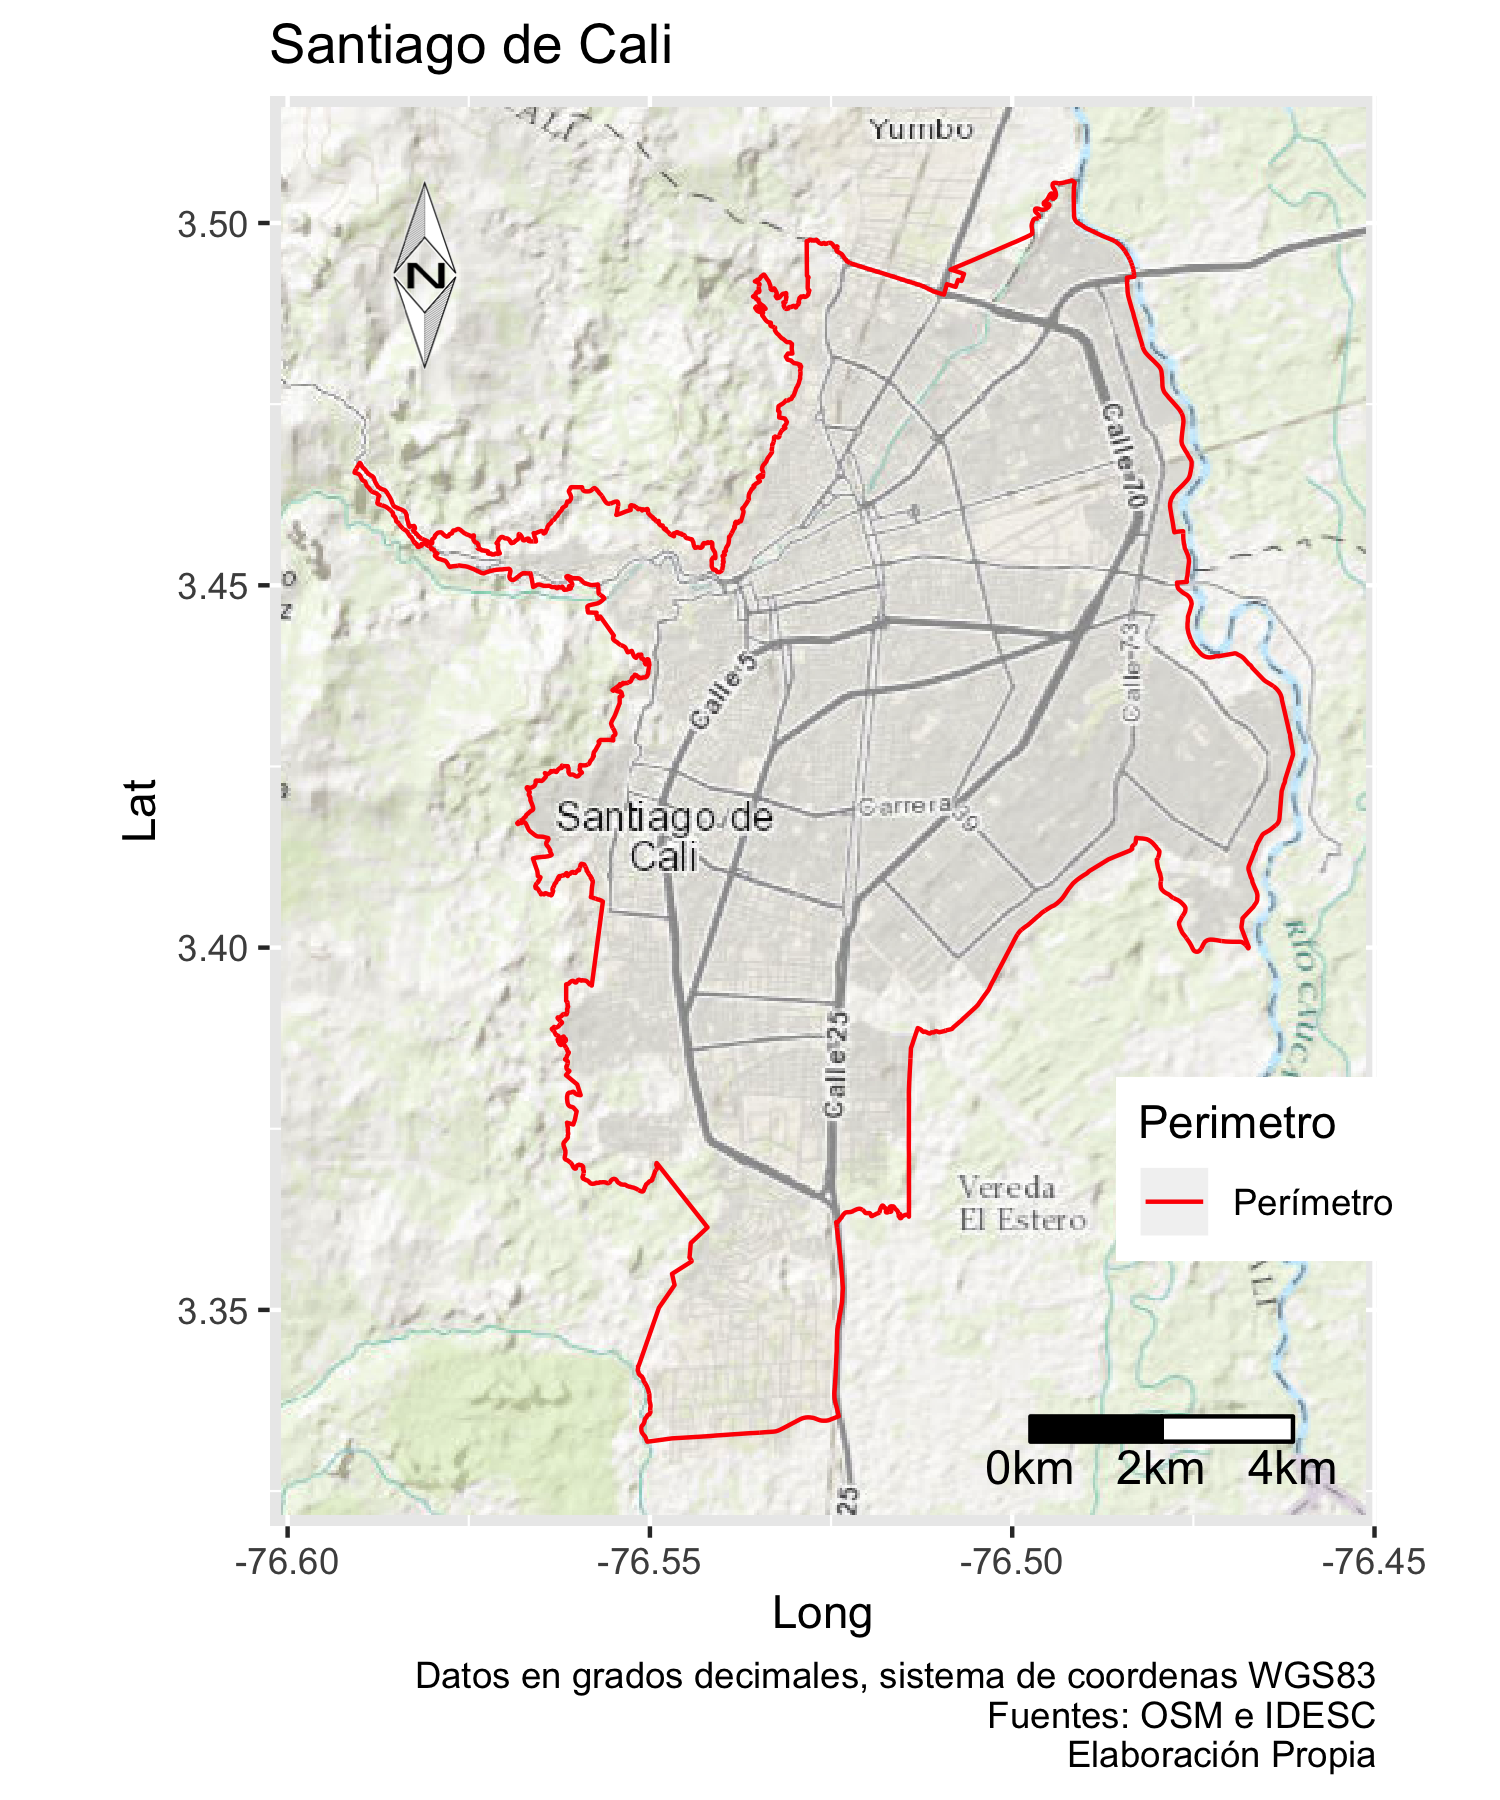
\includegraphics[width=0.9\linewidth]{tesis-unigis_files/figure-latex/mapa-area-1} 

}

\caption{Área de estudio. Perímetro urbano de Santiango de Cali}\label{fig:mapa-area}
\end{figure}

\section{Datos}\label{datos}

Se hizo uso de datos del Censo Arbóreo de 2015 (CA2015) (Alcaldía de
Cali, \protect\hyperlink{ref-ca2015cali}{2015}), el Censo de Población
de 2005 (CP2005) (DANE,
\protect\hyperlink{ref-censo_sistema_dane}{2005},
\protect\hyperlink{ref-geoportal_DANE}{2017}) y aspectos estructurales
del espacio público y privado de las unidades espaciales de análisis
tomados de la Infraestructura de Datos Espaciales de Santiago de Cali
(IDESC) (Alcaldía de Cali,
\protect\hyperlink{ref-geoportal_idesc}{2009}) y las bases de datos del
Plan de Ordenamiento Territorial (POT) del 2014 (Alcaldía de Cali,
\protect\hyperlink{ref-pot2014cali}{2014}).

\subsection{Datos de registros oficiales del
municipio}\label{datos-de-registros-oficiales-del-municipio}

La cartografía disponible en la IDESC (Alcaldía de Cali,
\protect\hyperlink{ref-geoportal_idesc}{2009}), incluye información
sobre los objetos geográficos naturales, de infraestructura urbana,
límites y divisiones político administrativas y la clasificación de
predios en cuanto a espacio público disponibles en coordenadas planas
del sistema MAGNA-SIRGAS-CALI (IGAG,
\protect\hyperlink{ref-igagMC2005}{2005}). Además está la base de datos
geográfica del POT (Alcaldía de Cali,
\protect\hyperlink{ref-pot2014cali}{2014}). Se seleccionaron conjuntos
de datos de equipamientos y espacio público contenido en la estructura
ecológica complementaria (EEC) que incluye cementerios, universidades,
EV de acceso no restringido aunque algunos sea predios privados
contenidos en EEC. De la IDESC se seleccionaron las capas de manzanas,
barrios, espacio público, humedales, ríos y corredores ambientales,
todas disponibles vía \emph{Web Feature Service} (WFS). En la figura
\ref{fig:capas-idesc} se muestra un mapa con las capas seleccionadas
para el realizar el procesamiento y los análisis.

\begin{figure}[H]

{\centering \includegraphics[width=1\linewidth]{QGIS/mapas/capas_analisis} 

}

\caption{Capas usadas para el procesamiento de los espacios verdes y las características de las manzanas}\label{fig:capas-idesc}
\end{figure}

\subsection{El censo arbóreo}\label{el-censo-arbuxf3reo}

En el año 2015 la ciudad de Santiago de Cali concretó la realización del
censo arbóreo (CA2015) que dejó como resultado una base de datos de
296,467 individuos censados (Alcaldía de Cali,
\protect\hyperlink{ref-ca2015cali}{2015}). Los datos dan cuenta de la
identificación de especies, georeferenciación de los individuos, sus
características dasométricas, de emplazamiento y estado fitosanitario.
Las variables contenidas en ese estudio se resumen en la tabla
\ref{tab:vars-AU}.

\begin{longtable}[]{@{}ll@{}}
\caption{\label{tab:vars-AU} Variables para caracterizar el
AU}\tabularnewline
\toprule
\begin{minipage}[b]{0.30\columnwidth}\raggedright\strut
variable\strut
\end{minipage} & \begin{minipage}[b]{0.42\columnwidth}\raggedright\strut
\{valores\}{[}unidades{]}\strut
\end{minipage}\tabularnewline
\midrule
\endfirsthead
\toprule
\begin{minipage}[b]{0.30\columnwidth}\raggedright\strut
variable\strut
\end{minipage} & \begin{minipage}[b]{0.42\columnwidth}\raggedright\strut
\{valores\}{[}unidades{]}\strut
\end{minipage}\tabularnewline
\midrule
\endhead
\begin{minipage}[t]{0.30\columnwidth}\raggedright\strut
id\_arbol\strut
\end{minipage} & \begin{minipage}[t]{0.42\columnwidth}\raggedright\strut
número entero único\strut
\end{minipage}\tabularnewline
\begin{minipage}[t]{0.30\columnwidth}\raggedright\strut
diametro copa\strut
\end{minipage} & \begin{minipage}[t]{0.42\columnwidth}\raggedright\strut
{[}m\textsuperscript{2}{]}\strut
\end{minipage}\tabularnewline
\begin{minipage}[t]{0.30\columnwidth}\raggedright\strut
altura arbol\strut
\end{minipage} & \begin{minipage}[t]{0.42\columnwidth}\raggedright\strut
{[}m{]}\strut
\end{minipage}\tabularnewline
\begin{minipage}[t]{0.30\columnwidth}\raggedright\strut
vitalidad\strut
\end{minipage} & \begin{minipage}[t]{0.42\columnwidth}\raggedright\strut
\{Regular, Sano, Seco, Muerto\}\strut
\end{minipage}\tabularnewline
\begin{minipage}[t]{0.30\columnwidth}\raggedright\strut
edad\strut
\end{minipage} & \begin{minipage}[t]{0.42\columnwidth}\raggedright\strut
\{Juvenil, Maduro, Longevo\}\strut
\end{minipage}\tabularnewline
\begin{minipage}[t]{0.30\columnwidth}\raggedright\strut
emplazamiento\strut
\end{minipage} & \begin{minipage}[t]{0.42\columnwidth}\raggedright\strut
\{Anden, Bahias de estacionamiento, Bulevares, Corredor Ferreo,
Escenario deportivo y/o Cultural, Glorieta, Parque Urbano, Paseos,
Plaza, Plazoleta, Ronda de rios, Rondas de canales, Separador
Vial\}\strut
\end{minipage}\tabularnewline
\begin{minipage}[t]{0.30\columnwidth}\raggedright\strut
vegetación\strut
\end{minipage} & \begin{minipage}[t]{0.42\columnwidth}\raggedright\strut
\{Arbol, Arbusto, Bambu, Muerto, Palma, Planta arbustiva, Seco\}\strut
\end{minipage}\tabularnewline
\begin{minipage}[t]{0.30\columnwidth}\raggedright\strut
Este\strut
\end{minipage} & \begin{minipage}[t]{0.42\columnwidth}\raggedright\strut
{[}m{]} MAGNA - SIRGAS-CALI\strut
\end{minipage}\tabularnewline
\begin{minipage}[t]{0.30\columnwidth}\raggedright\strut
Norte\strut
\end{minipage} & \begin{minipage}[t]{0.42\columnwidth}\raggedright\strut
{[}m{]} MAGNA - SIRGAS-CALI\strut
\end{minipage}\tabularnewline
\bottomrule
\end{longtable}

Existe una diferencia de 10 años entre censo de población de 2005 y el
censo arbóreo de la ciudad de Cali. Aunque esto pueda parecer una
situación que reduce la legitimidad de los resultados que se hallen en
este estudio, autores como Boone, Cadenasso, Grove, Schwarz, y Buckley
(\protect\hyperlink{ref-boone2010landscape}{2010}) y Schwarz et~al.
(\protect\hyperlink{ref-schwarz_trees_2015}{2015}) reconocen que los
paisajes que vemos hoy son legados de patrones de consumo pasados, y que
en el caso de la vegetación urbana tratamos con organismos de larga vida
que pueden tardar mucho tiempo en establecerse y crecer. En contraste,
la estructura social de las ciudades puede cambiar más rápidamente.

Atendiendo a estos argumentos se excluyó de la base de datos del CA2015
árboles jóvenes del inventario, que no estaban ahí en 2005. Aunque toda
la vegetación aporta beneficios ambientales a los habitantes, en este
estudio se descartó la vegetación arbustiva y los árboles, palmas y
bambú de menos de 1.9 m de altura para circunscribirse a los individuos
más desarrollados.

Una vez aplicado este filtro se cuenta con 203,112 individuos.

\subsection{El censo de población}\label{el-censo-de-poblaciuxf3n}

Los datos del CP2005 están disponibles en las unidades censales (sector,
sección, manzana) a través del sistema de consulta web (DANE,
\protect\hyperlink{ref-censo_sistema_dane}{2005}). Estos datos sirven
para caracterizar la población con base en indicadores sobre rasgos de
las personas, aspectos sobre el uso del suelo y los tipos de vivienda.
Las variables disponibles para el análisis están resumidas en las tablas
\ref{tab:vars-poblacion} y \ref{tab:vars-vivienda}.

El otro componente de los datos es la cartografía censal del DANE (DANE,
\protect\hyperlink{ref-geoportal_DANE}{2017}) disponible para las
diferentes unidades espaciales de agregación en el sistema de
coordenadas WGS84. Para el análisis se tiene en cuenta todos las
unidades censales que se interceptan con el perímetro urbano disponible
en la IDESC, pues el censo arbóreo se limitó a este perímetro.(ver
figura \ref{fig:su-periurbano})

\begin{longtable}[]{@{}ll@{}}
\caption{\label{tab:vars-poblacion} Variables sobre la
población}\tabularnewline
\toprule
\begin{minipage}[b]{0.20\columnwidth}\raggedright\strut
variable\strut
\end{minipage} & \begin{minipage}[b]{0.43\columnwidth}\raggedright\strut
\{valores\}{[}unidades{]}\strut
\end{minipage}\tabularnewline
\midrule
\endfirsthead
\toprule
\begin{minipage}[b]{0.20\columnwidth}\raggedright\strut
variable\strut
\end{minipage} & \begin{minipage}[b]{0.43\columnwidth}\raggedright\strut
\{valores\}{[}unidades{]}\strut
\end{minipage}\tabularnewline
\midrule
\endhead
\begin{minipage}[t]{0.20\columnwidth}\raggedright\strut
Pertenencia Étnica\strut
\end{minipage} & \begin{minipage}[t]{0.43\columnwidth}\raggedright\strut
{[}personas{]}\{indígenas, ROM, gitanos, raizales del Archipiélago de
San Andrés, Providencia y Santa Catalina, palenqueros de San Basilio,
afrocolombianos\}\strut
\end{minipage}\tabularnewline
\begin{minipage}[t]{0.20\columnwidth}\raggedright\strut
Con alguna limitación\strut
\end{minipage} & \begin{minipage}[t]{0.43\columnwidth}\raggedright\strut
{[}personas{]}\{sí,no\}\strut
\end{minipage}\tabularnewline
\begin{minipage}[t]{0.20\columnwidth}\raggedright\strut
Con estudios superior o postgrado\strut
\end{minipage} & \begin{minipage}[t]{0.43\columnwidth}\raggedright\strut
{[}personas{]}\strut
\end{minipage}\tabularnewline
\begin{minipage}[t]{0.20\columnwidth}\raggedright\strut
Ningún estudio\strut
\end{minipage} & \begin{minipage}[t]{0.43\columnwidth}\raggedright\strut
{[}personas{]}\strut
\end{minipage}\tabularnewline
\bottomrule
\end{longtable}

\begin{longtable}[]{@{}ll@{}}
\caption{\label{tab:vars-vivienda} Variables sobre la las
viviendas}\tabularnewline
\toprule
\begin{minipage}[b]{0.24\columnwidth}\raggedright\strut
variable\strut
\end{minipage} & \begin{minipage}[b]{0.37\columnwidth}\raggedright\strut
\{valores\}{[}unidades{]}\strut
\end{minipage}\tabularnewline
\midrule
\endfirsthead
\toprule
\begin{minipage}[b]{0.24\columnwidth}\raggedright\strut
variable\strut
\end{minipage} & \begin{minipage}[b]{0.37\columnwidth}\raggedright\strut
\{valores\}{[}unidades{]}\strut
\end{minipage}\tabularnewline
\midrule
\endhead
\begin{minipage}[t]{0.24\columnwidth}\raggedright\strut
tipo vivienda\strut
\end{minipage} & \begin{minipage}[t]{0.37\columnwidth}\raggedright\strut
\{Casa,Casa indígena,Apartamento,Tipo cuarto,Otro tipo de
vivienda\}{[}viviendas{]}\strut
\end{minipage}\tabularnewline
\begin{minipage}[t]{0.24\columnwidth}\raggedright\strut
uso vivienda\strut
\end{minipage} & \begin{minipage}[t]{0.37\columnwidth}\raggedright\strut
\{Uso Vivienda.Uso Unidad Económica,Uso LEA\}{[}predios{]}\strut
\end{minipage}\tabularnewline
\begin{minipage}[t]{0.24\columnwidth}\raggedright\strut
cantidad predios\strut
\end{minipage} & \begin{minipage}[t]{0.37\columnwidth}\raggedright\strut
{[}predios{]}\strut
\end{minipage}\tabularnewline
\begin{minipage}[t]{0.24\columnwidth}\raggedright\strut
cantidad viviendas\strut
\end{minipage} & \begin{minipage}[t]{0.37\columnwidth}\raggedright\strut
{[}viviendas{]}\strut
\end{minipage}\tabularnewline
\bottomrule
\end{longtable}

La unidad espacial de análisis sobre la cual se harán todas las
agregaciones es el sector urbano (SU) de la cartografía censal 2005.

\begin{figure}[H]

{\centering 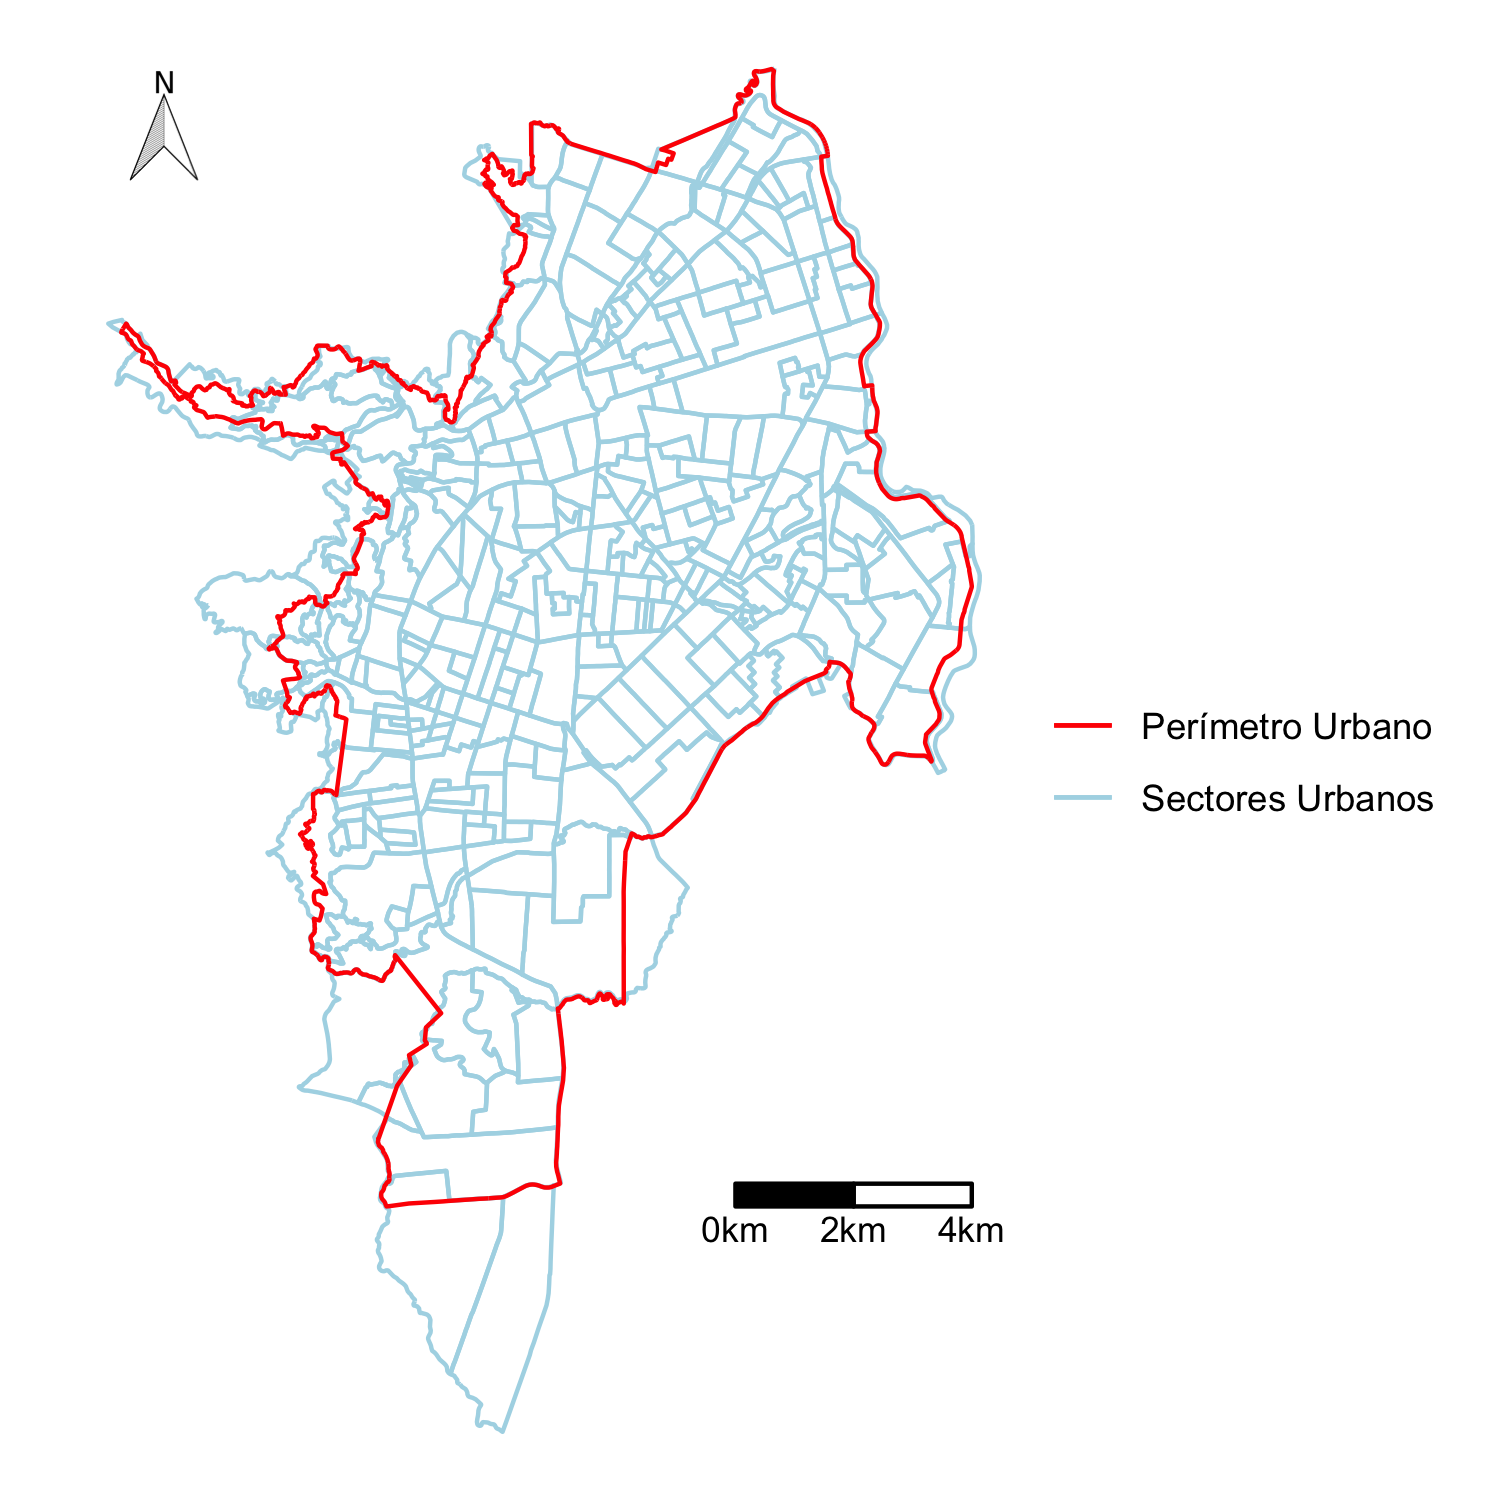
\includegraphics[width=0.9\linewidth]{tesis-unigis_files/figure-latex/su-periurbano-1} 

}

\caption{Sectores urbanos y périmetro urbano de Santiago de Cali}\label{fig:su-periurbano}
\end{figure}

\section{Métodos y técnicas}\label{muxe9todos-y-tuxe9cnicas}

Este trabajo se concentró en indagar en particular sobre la justicia
ambiental distributiva por medio de modelos estadísticos de regresión y
geoestadísticos usados ampliamente en la literatura revisada (Gibbons y
Overman, \protect\hyperlink{ref-gibbons_mostly_2012}{2012}; Heynen
et~al., \protect\hyperlink{ref-heynen_political_2006}{2006}; Landry y
Chakraborty, \protect\hyperlink{ref-landry_street_2009}{2009}; LeSage y
Pace, \protect\hyperlink{ref-lesage_biggest_2014}{2014}; Pacheco,
\protect\hyperlink{ref-PACHECO2013121}{2013}; Schwarz et~al.,
\protect\hyperlink{ref-schwarz_trees_2015}{2015}; Shanahan et~al.,
\protect\hyperlink{ref-shanahan_socio-economic_2014}{2014}; Vásquez
Fuentes y Romero Aravena,
\protect\hyperlink{ref-vasquez_fuentes_vegetacion_2008}{2008}; Zhou y
Kim, \protect\hyperlink{ref-zhou_social_2013}{2013}). Se busca probar
que existe un sesgo en la distribución de un beneficio ambiental (AU y
EV) explicado por alguna variable socioeconómica o estructural. Desde la
modelación estadística esto se logra encontrando predictores con
coeficientes significativos en la regresión lineal. Si exsite un patrón
espacial que puede ser includo en la modelación para mejorar la
estimación de los coeficiente de la regresión, su inclusión debe mejorar
las condiciones de normalidad y homocedasticidad de los residuos de la
regresión.

Para detectar agrupaciones de unidades geográficas con características
homogéneas donde intervenir y disminuir las inequidades en el acceso a
servicios ambientales se complementan los análisis con el uso de mapas
de LISA (Talen y Anselin,
\protect\hyperlink{ref-talen_assessing_1998}{1998}).

El diagrama de la figura \ref{fig:flujograma} sintetiza el análisis
propuesto, compuesto de las siguientes actividades:

\begin{enumerate}
\def\labelenumi{\arabic{enumi}.}
\tightlist
\item
  Preparación de los datos: construcción de tablas, estandarización de
  las variables categóricas, sistemas de coordenadas y la identificación
  de valores atípicos o inconsistentes en los datos.
\item
  Procesamiento y análisis estadístico: cálculo de indicadores de
  cobertura, acceso y variables socioeconómicas. Cálculo de estadísticos
  para probar normalidad, normalización de las variables e indicadores,
  cálculos de coeficientes de correlación Pearson y de Spearman entre
  todos los pares de variables.
\item
  Análisis exploratorio: hacer uso de gráficas estadísticas, mapeos y
  mapas para evaluar y seleccionar los indicadores a usar en un modelo
  de regresión lineal.
\item
  Seleccionar los mejores predictores con base en coeficientes de
  correlación.
\item
  Seleccionar los SU a incluir con base la coincidencia con las capas de
  AU y EV.
\item
  Construir y evaluar los modelos de regresión lineal.
\item
  Contruir matrices de vencidad \(W\) para incluir restricciones
  espaciales al modelo.
\item
  Probar autocorrelación espacial usando Moran'I en los residuos de los
  modelos de regresión lineal con dos diseños de matriz \(W\). Si la
  prueba muestra una correlación y un valor de significancia alta, se
  prueban modelos tipo SAR, SEM o SD para comparar su desempeño.
\item
  Selección del modelo que mejor se ajusta usando métricas de error y de
  ajuste como R\textsuperscript{2} y el criterio de Akaike.
\item
  Graficar mapas de LISA para caraterizar los patrones de agrupación de
  las variables del los modelos mejor ajustados.
\end{enumerate}

\begin{figure}[H]

{\centering 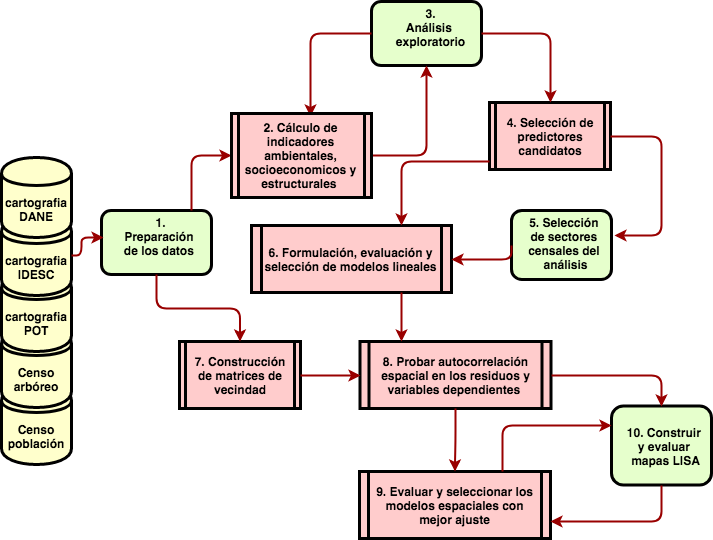
\includegraphics[width=1\linewidth]{images/flujograma} 

}

\caption{Diagrama de flujo de la metodología}\label{fig:flujograma}
\end{figure}

\subsection{Procesamiento de datos}\label{procesamiento-de-datos}

El procesamiento de los datos se realizó principalmente en R (R Core
Team, \protect\hyperlink{ref-R-base}{2017}). Se usó
\href{http://www.qgis.org/es/site/}{QGIS} para conectarse a los
servicios WFS del IDESC y previsualizar las capas de información
geográfica recolectada y la realización de algunos de los mapas
detallados. Para cargar y manipular los datos espaciales se hizo uso de
las librerías \texttt{rgdal} (Bivand, Keitt, y Rowlingson,
\protect\hyperlink{ref-R-rgdal}{2017}), \texttt{rgeos} (Bivand y Rundel,
\protect\hyperlink{ref-R-rgeos}{2018}) y \texttt{sp} (Pebesma y Bivand,
\protect\hyperlink{ref-R-sp}{2018}). En el apéndice \ref{rinfo} se
encuentra la información completa de la sesión de R.

El código que implementa los análisis está dividido en archivos para
facilitar su lectura, cada uno de los cuales se encargan de transformar
los datos de las fuentes y construir estructuras de datos necesarias
para realizar las regresiones, las gráficas y los análisis de tipo
estadístico y geoestadístico.

El código y los datos están disponibles en el
\href{https://github.com/correajfc/R-CP2005-CA2015}{repositorio de
GitHub} en \url{https://github.com/correajfc/R-CP2005-CA2015}.

\subsection{Cálculo de métricas de acceso a servicios
ambientales}\label{cuxe1lculo-de-muxe9tricas-de-acceso-a-servicios-ambientales}

\subsubsection{Indicadores de beneficios del arbolado
urbano}\label{indicadores-de-beneficios-del-arbolado-urbano}

\begin{figure}[H]

{\centering 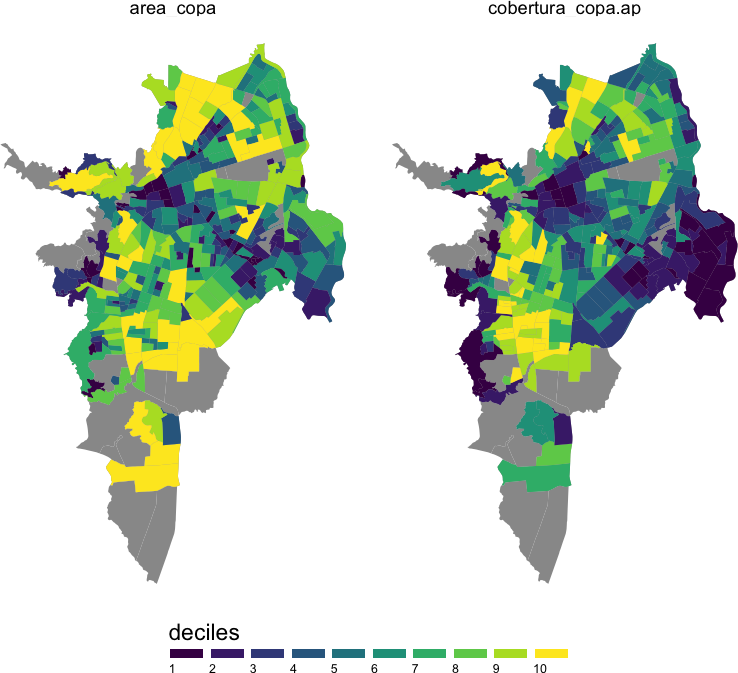
\includegraphics[width=0.8\linewidth]{tesis-unigis_files/figure-latex/mapa-copa-dep-1} 

}

\caption{Sectores urbanos de las variables dependientes sobre cobertura de copa}\label{fig:mapa-copa-dep}
\end{figure}

Entre los distintos indicadores desarrollados para capturar la extensión
y distribución de los servicios ambientales, la cobertura de copas ha
probado ser sensible y eficaz para cuantificar hasta qué punto los
árboles y bosques están proporcionando servicios críticos a los
residentes (Nowak et~al.,
\protect\hyperlink{ref-nowak_sustaining_2010}{2010}).

En este trabajo se usaron dos variantes de la cobertura de copa, una de
orden global y otra local respectivamente: el área de copa en
metros\textsuperscript{2} (\texttt{area\_copa}) y la cobertura de copa
como porcentaje del área pública total (\texttt{cobertura\_copa.ap}),
conformada por la vías y calles más el área de espacio públicos (ver
figura \ref{fig:mapa-copa-dep}).

\subsubsection{Índices de acceso a espacios
verdes}\label{uxedndices-de-acceso-a-espacios-verdes}

En este estudio se usaron dos métricas de acceso a espacios verdes. El
primero es el índice contenedor porcentual (ecuación \eqref{eq:n-cont}),
catalogado como una medida de acceso local a la unidad espacial de
análisis, ampliamente usado en la literatutra (Talen y Anselin,
\protect\hyperlink{ref-talen_assessing_1998}{1998}).

\textbf{índice contenedor porcentual} (area\_ep.porcentaje)

\begin{equation}
A^{C_p}_i =1/a_i\sum_j{s_j} \;  \; \forall  j \in I
\label{eq:n-cont}
\end{equation}

donde \(s_j\) es el área de cada espacio verde \(j\) que pertenece al
conjunto \(I\) de EV dentro del sector \(i\) y \(a_i\) es el área del
sector \(i\).

El segundo índice (ecuación \eqref{eq:areas-dists}) es una propuesta de
este estudio basada en el trabajo de Nesbitt y Meitner
(\protect\hyperlink{ref-nesbitt_exploring_2016}{2016}) en el que se
calcula la distancia euclide a los EV desde el centroide de la unidad de
análisis, incorporando recomendaciones de la Organización Mundial de la
Salud sobre establacer la relación entre distancia y calidad del acceso
usando el área del EV (WHO, \protect\hyperlink{ref-who2016urban}{2016})
y los índice propuestos por Zhou y Kim
(\protect\hyperlink{ref-zhou_social_2013}{2013}) de un radio de búsqueda
de EVs accesibles, sin importar si este está dentro de la unidad
espacial a caraterizar.

Este índice define el acceso como una relación entre la distancia y la
cantidad de espacio disponible en el radio de búsqueda definido desde el
centroide del SU. La figura \ref{fig:mapa-rango1km} muestra gráficamente
como existen EVs que caen la intersección de los radios de búsqueda de
multiples sectores urbanos, lo que implica que benefician a varios de
ellos a la vez, y es por esa razón que el índice expresa una dimensión
del acceso no confinada a la unidad espacial.

\textbf{razón área disponible distancia} (ia.areas.dist)

\begin{equation}
\bar{A}^{AD}_i= \frac{\sum_{\int R_b }{s_j}}{\sum_{\int R_b }{d_{ij}}}  \;  \; \forall  j \in I_{R_b} \; 
\label{eq:areas-dists}
\end{equation}

donde \(R_b\) es el radio de búsqueda, \(s_j\) es el área de cada
espacio verde \(j\), \(d_{ij}\) es la distancia del centriode del sector
\(i\) al espacio \(j\) que pertenecen al conjunto \(I_{R_b}\) de EVs en
el radio de búsqueda.

\begin{figure}[H]

{\centering 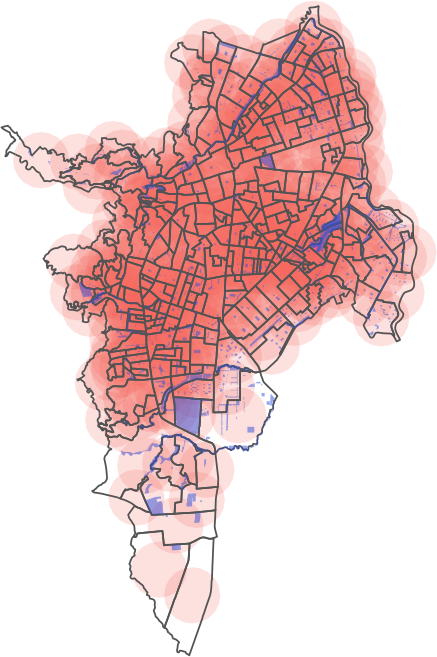
\includegraphics[width=0.7\linewidth]{tesis-unigis_files/figure-latex/mapa-rango1km-1} 

}

\caption{Espacios verdes y radio de búsqueda de 1 km desde los centriodes del SU}\label{fig:mapa-rango1km}
\end{figure}

\subsection{Cálculo de métricas sobre la
población}\label{cuxe1lculo-de-muxe9tricas-sobre-la-poblaciuxf3n}

\subsubsection{Características de la
población}\label{caracteruxedsticas-de-la-poblaciuxf3n}

La tabla \ref{tab:vars-poblacion} muestra los valores de la variable de
etnicidad. Al hacer los conteos por pertencia a un grupo etnico para
toda la ciudad (ver tabla \ref{tab:totales-poblacion}), se observa el
bajo número de personas que pertenecen al pueblo Rom (gitanos),
Palenqueros de San Basilio (departamento de Bolívar) y de Raizales del
Archipiélago de San Andrés, Providencia y Santa Catalina (SAI) y a la
población indígena, por lo que son descartados del análisis.

\begin{table}[t]

\caption{\label{tab:totales-poblacion}Totales de población por grupo étnico en la ciudad de Cali}
\centering
\begin{tabular}{ll}
\toprule
Tipo & Cantidad\\
\midrule
Población Total & 2,027,024\\
Población afrodescendiente, negros o mulatos & 530,990\\
Población indígena & 9,195\\
Población Rom & 690\\
Población Palenqueros & 1\\
\addlinespace
Población raizales de SAI & 851\\
\bottomrule
\end{tabular}
\end{table}

Las variables del CP2005 seleccionadas para el análisis se muestran en
la figura \ref{fig:mapas-poblacion-deciles}.

\begin{figure}[p]

{\centering 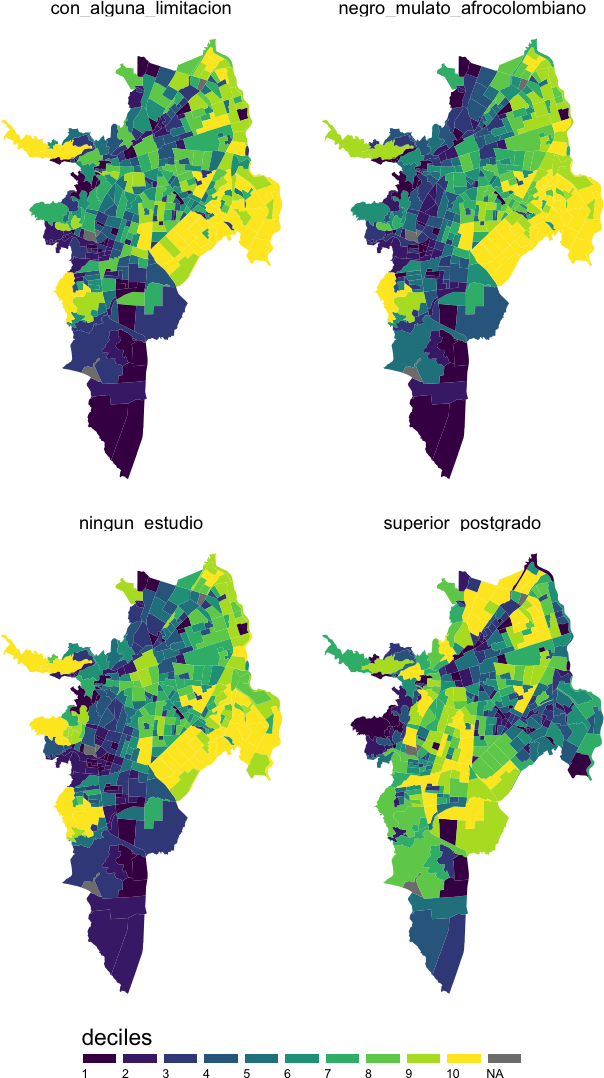
\includegraphics[width=0.7\linewidth]{tesis-unigis_files/figure-latex/mapas-poblacion-deciles-1} 

}

\caption{Mapas de las variables de población seleccionadas (en deciles).}\label{fig:mapas-poblacion-deciles}
\end{figure}

Además de las variables seleccionadas se calculó la densidad de
población dado que los árboles compiten por el espacio con los seres
humanos y es de esperar que a mayor cantidad de personas haya menos
lugar para los árboles. Se calcularon indicadores porcentuales respecto
de la población total de cada unidad geográfica para facilitar la
comparaciones y acentuar las diferencias entre los SU (figura
\ref{fig:mapas-poblacion-mod-deciles}).

\begin{figure}[H]

{\centering 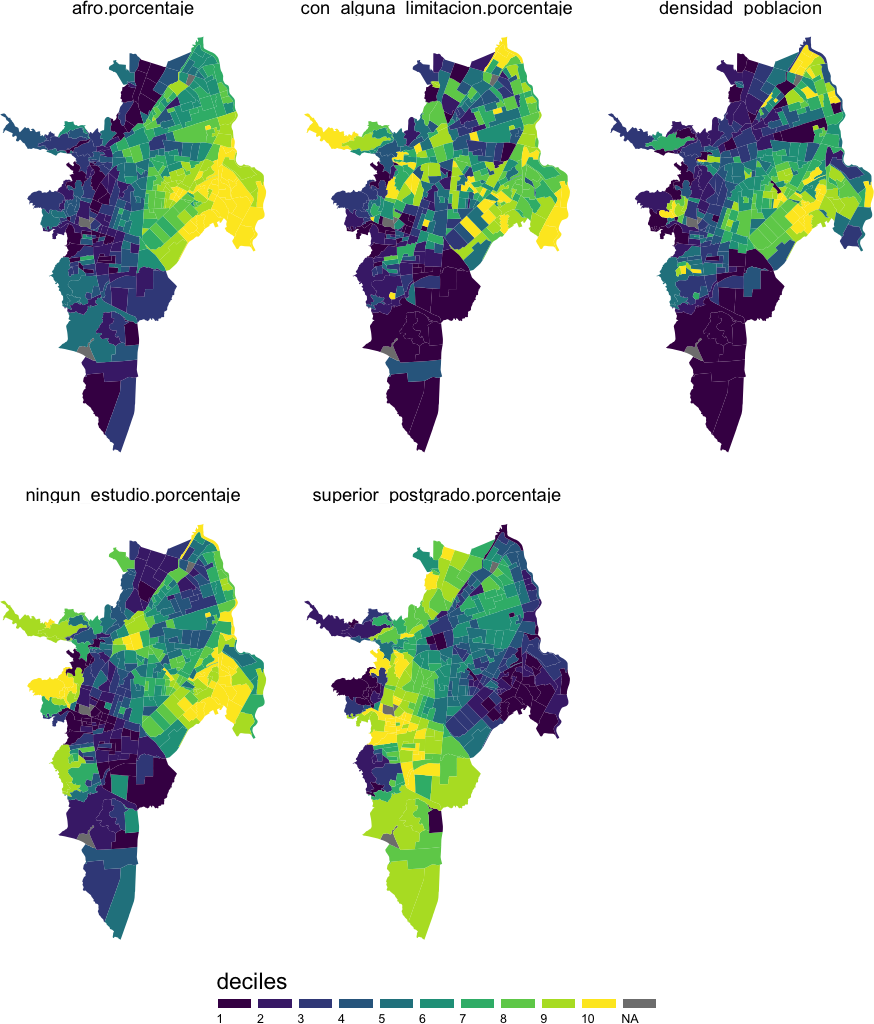
\includegraphics[width=0.9\linewidth]{tesis-unigis_files/figure-latex/mapas-poblacion-mod-deciles-1} 

}

\caption{Mapas de las variables de población seleccionadas como porcentajes (en deciles)}\label{fig:mapas-poblacion-mod-deciles}
\end{figure}

\subsubsection{Características de las
viviendas}\label{caracteruxedsticas-de-las-viviendas}

Además de las rasgos étnicos, condiciones de escolaridad y limitaciones
de la población, el CP2005 tiene disponibles datos sobre el tipo de
viviendas (casa, apartamento, tipo cuarto, casa indígena, otros), y el
uso habitacional, comercial y la cantidad de lugares especiales de
alojamiento\footnote{Corresponden a las diferentes unidades que
  desempeña una función de interés público, que puede ser benéfico o
  docente} (LEA) dado a los predios. La vocación comercial o residencial
de un barrio puede ser un factor en el desarrollo del arbolado urbano o
de las disposiciones urbanísticas de la ciudad en relación a EVs, ya sea
por las condiciones físicas como por la intervención de sus habitantes.
Estas variables pueden también expresarse como porcentaje de la cantidad
de predios de vivienda según los tipos o como porcentaje de la cantidad
de predios según su uso: vivienda, unidad económica o LEA. La variable
LEA presenta una distribución uniforme, por lo que se descarta para los
análisis de regresión (ver los gráficos por sector urbano en la figura
\ref{fig:mapas-usopredios-cont}).

\begin{figure}[H]

{\centering 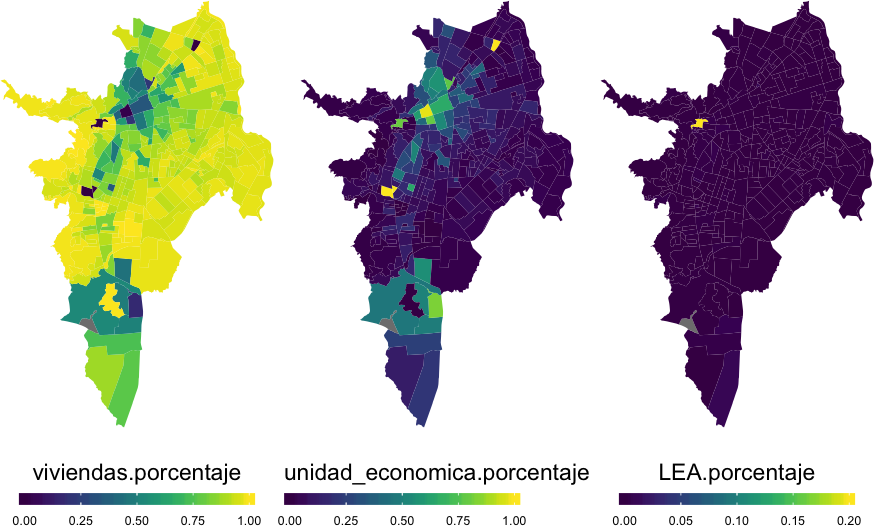
\includegraphics[width=0.8\linewidth]{tesis-unigis_files/figure-latex/mapas-usopredios-cont-1} 

}

\caption{Mapas de las variables sobre el tipo de uso de los predios como porcentaje de la cantidad de predios (escala contínua)}\label{fig:mapas-usopredios-cont}
\end{figure}

\subsection{Criterios y selección de sectores
censales}\label{criterios-y-selecciuxf3n-de-sectores-censales}

Se establecieron criterios para la \textbf{exclusión} de datos para el
análisis de regresión que evitan incluir SUs atípicos:

\begin{itemize}
\tightlist
\item
  sectores sin personas
\item
  sectores sin viviendas
\item
  sectores con área de espacio público mayor que el 80 \% del área del
  sector
\item
  sectores con área de calle mayor que el 80 \% del área del sector
\item
  sectores área privada mayor que el 90 \% del área del sector
\item
  sectores con una porción mayor al 60\% por fuera del perímetro urbano
\end{itemize}

Los sectores excluidos del análisis se muestran en la figura
\ref{fig:mapa-excluidos}.

\begin{figure}[H]

{\centering 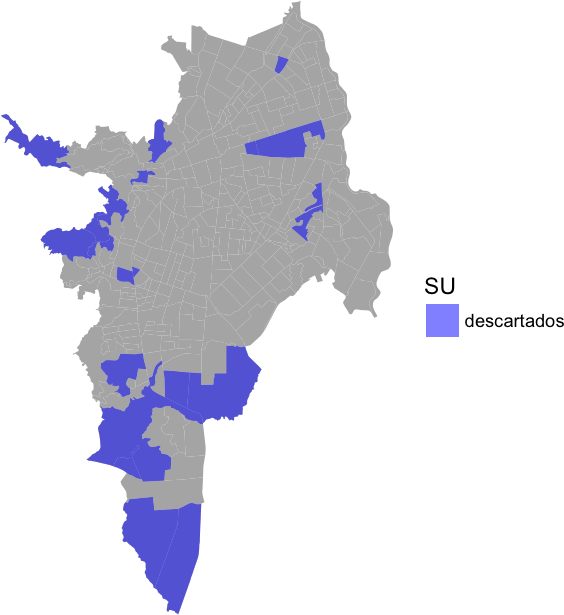
\includegraphics[width=0.6\linewidth]{tesis-unigis_files/figure-latex/mapa-excluidos-1} 

}

\caption{Sectores excluidos}\label{fig:mapa-excluidos}
\end{figure}

\subsection{Selección de variables dependientes para las regresiones
lineales}\label{selecciuxf3n-de-variables-dependientes-para-las-regresiones-lineales}

Las variables incluidas en los modelos lineales deben cumplir una serie
de condiciones deseables para ser elegidas como candidatas:

\begin{itemize}
\tightlist
\item
  Mostrar una correlación moderada o fuerte\footnote{En este trabajo se
    considera moderado a valores superiores y al rededor de 0.6 en los
    coeficientes de correlación. Aunque definir cualitativamente rangos
    de un coeficiente de correlación es arbitrario, es posible
    definirlos y usarlos con criterio. Se puede estar acuerdo que
    correlaciones menores a 0.1 indica una relación insignificante y que
    mayores 0.9 una muy fuerte, pero los valores intermedios son
    discutibles.}
\item
  Las variables independientes o predictoras \textbf{no} deben estar
  fuertemente correlacionadas entre ellas.
\item
  Las observaciones deben ser \textbf{independientes}\footnote{Significa
    que no debe existir relación espacial o temporal entre los
    diferentes sectores. Justamente esto se pone a prueba con los test
    estadísticos y los gráficos de diagnóstico sobre la distribución de
    los residuos de la regresión: se espera que dicha dependencia esté
    motivada por la vecindad de los sectores.}
\end{itemize}

Para garantizar que las variables no están correlacionadas entre sí, se
usó el coeficiente de correlación de Pearson para detectar relaciones
lineales, y el coeficiente de Spearman para detectar relaciones en que
exhiben relaciones no lineales.

Para seleccionar las variables que mejor predicen la variable
dependiente se tuvo en cuenta las restricciones de colinealidad entre
las variables dependientes.

Para los modelos de regresión se usaron transformaciones logarítmicas o
de raíz cuadra para eliminar no linealidades entre las variables
dependientes y las independientes, y reducir posibles fenómenos de
heterocedasticidad debido a estas no-linealidades.

Dividir o multiplicar por alguna constante no tiene ningún efecto en la
calidad de las estimaciones , pero sí sobre los coeficientes de la
regresión. Esto suele ser sensible a la hora de interpretar los cambios
marginales de cada una de las variables independientes y su efecto sobre
la variable dependiente. Sin embargo, lo que interesa para este estudio
no es la interpretación de esos cambio sino la importancia relativa de
cada variable y comparar los cambios de los coeficientes de regresión
para el ajuste de cada modelo y/o las mejoras que pueda operar un
modelos autorregresivo en caso de encontrase autocorrelación en los
residuos de la regresión lineal. Por esta razón, normalizar los valores
puede ser una ventaja pues mantiene los coeficiente mejor acotados. La
normalización se aplicó posterior a las transformaciones propuestas y se
realizó dividiendo por el máximo valor de los datos de cada variable
para mantener valores en el intervalo {[}0,1{]}, dado que los valores
son todos iguales o mayores que 0.

Los test aplicados para verificar las condiciones de un buen ajuste (no
hay sesgos en el estimador o una mala especificación del modelo) de un
modelo lineal son:

\begin{itemize}
\tightlist
\item
  La media de los residuos es 0 o muy cercana.
\item
  La distribución de los residuos es normal.
\item
  Los residuos muestran homocedasticidad (la varianza es constante)
\end{itemize}

Para verificar la normalidad de los residuos se hace uso del test de
Shapiro--Wilk (Shapiro y Wilk,
\protect\hyperlink{ref-shapiro1965analysis}{1965} ) y para la verificar
si existe homocedasticidad el test de Breusch--Pagan (Breusch y Pagan,
\protect\hyperlink{ref-breusch1979simple}{1979}).

\subsection{Análisis geoestadísticos}\label{geostat}

Para los análisis geoestadísticos, se hizo uso de modelos autoregresivos
para obtener mejoras en la estimación de los coeficientes y en el ajuste
de los modelos lineales, cuando existío algún tipo de autocorrelación
espacial en los residuos. Todas estas aproximaciones introducen una
matriz de \(W_{n \times n}\), donde \(n\) es el número de sitios, que
captura la influencia de las variables en relación con su proximidad.
Esta matriz \(W\) es una estructura que restringe la influencia \emph{a
priori} en los modelos. Para observar el efecto que tiene esta matriz
sobre los resultados del modelo se usaron 2 matrices distintas, y se
escogió la que produjo el mejor ajuste.

Para los análisis espaciales se usó la librería \texttt{spdep} (Bivand,
\protect\hyperlink{ref-R-spdep}{2017})

\subsubsection{Matrices de vecindad}\label{matrices-de-vecindad}

\begin{figure}[H]

{\centering 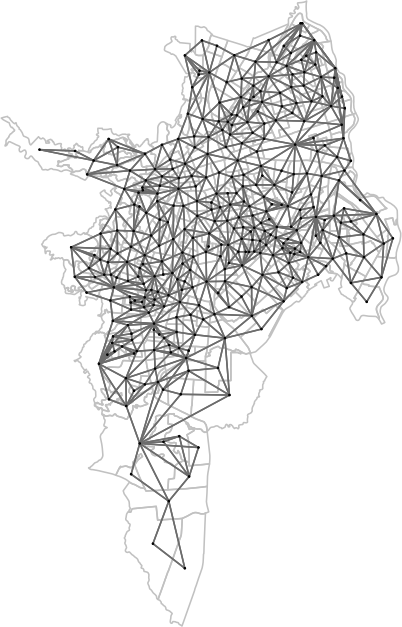
\includegraphics[width=0.6\linewidth]{tesis-unigis_files/figure-latex/w-su-todos-1} 

}

\caption{Grafo de vecindad entre todos los SU de la ciudad de Cali}\label{fig:w-su-todos}
\end{figure}

La matriz \(W\) representa la topología de vecindad entre las unidades
geográficas. Existen en la literatura diferentes tipos de vecindad:
\emph{rook}, \emph{bishop} y \emph{queen} son las más referenciadas.
Esta vecindad está representada en la matriz con 1 cuando existe
vecindad y 0 cuando no. Otra forma de cuantificar la interacción de esa
vecindad es usando una matriz de inversos de la distancia entre los
centroides de las unidades geográficas (\(W_d\)), con el fin de atenuar
la interacción entre sectores muy alejados y tener una variable continua
que representa esa influencia. En la figura \ref{fig:w-su-todos} se
muestra la representación de grafo de la matriz \(W_q\) de SUs vecinos
que comparten un lado del polígono (vecindad \emph{queen}) en la ciudad
de Cali.

Las regresiones se realizan sobre un subconjunto de los SUs, y por tanto
la estructura de esta matriz tuvo esto en cuenta.

\subsubsection{Autocorrelación
espacial}\label{autocorrelaciuxf3n-espacial}

Para indagar sobre la información o patrones espaciales de los residuos
de los modelos de regresión se usó el índice de Moran'I (ecuación
\eqref{eq:moranI}). El índice de Moran'I es el coeficiente de correlación
para la relación entre una variable y sus valores circundantes. Cuando
se encuentra una correlación espacial significativa en los residuos,
esto sugiere que agregando esa estructura de vecindad al modelo es
posible obtener una estimación más eficiente de los coeficientes, y en
consecuencia una estimación más confiable de los coeficientes. En este
estudio no se hace inferencia de una población por una muestra, se
calcularon coeficientes sobre el total de la población, y por tanto los
coeficientes pueden interpretarse como la fuerza de esa relación.

\begin{equation}
 I=\frac {N}{\sum _{i}\sum _{j}w_{ij}} \frac {\sum _{i}\sum _{j}w_{ij}(X_{i}-{\bar {X}})(X_{j}-{\bar {X}})}{\sum _{i}(X_{i}- \bar{X})^{2}}
\label{eq:moranI}
\end{equation}

donde \(N\) es el número de unidades espaciales indexados por \(i\) y
\(j\); \(X\) es la variable de interés; \(\bar {X}\) es la media de
\(X\); y \(w_{ij}\) es un elemento de una matriz de pesos espaciales
\(W\). Un valor de 0 de Moran'I indica un patrón espacial aleatorio. Si
existe autocorrelación los valores son positivos y el máximo es 1. Si
los valores son negativos se dice que existe dispersión, siendo -1 el
mínimo valor posible representando la dispersión perfecta. El valor
\textbf{\(p\)} del test expresa el grado de certeza sobre el valor del
estadístico, si el valor límite de significancia es menor que
\(\alpha = 0.05\)

\subsubsection{Indicadores Locales de Asociación Espacial
(LISA)}\label{indicadores-locales-de-asociaciuxf3n-espacial-lisa}

Dado que Morán'I es una suma de productos cruzados individuales es
explotado para formular los indicadores locales de asociación espacial
(LISA). Estos permiten evaluar la agrupación de las unidades
individuales mediante el cálculo de la Moran local para cada unidad
espacial y la evaluación de la significación estadística de este
indicador (Anselin, \protect\hyperlink{ref-anselin1995local}{1995}).

Estos mapas en conjunto con el resultado numérico de los LISA
z-normalizado y el \(p\)-valor permiten identificar agrupaciones
espaciales. Las regiones resaltadas en rojo tienen valores altos de la
variable y tienen vecinos con valores altos también (\emph{high-high}).
El área azul (\emph{low-low}) son los grupos que presentan valores bajos
al igual que sus vecinos. Mientras que las regiones azul pálido son
\emph{low-high} y las áreas rosadas son \emph{high-low} muestran
correlación negativa, es decir valores muy diferentes a los de sus
vecinos. Las regiones fuertemente coloreadas son aquellas que
contribuyen significativamente a un resultado positivo de
autocorrelación espacial global, mientras que los colores más claros
contribuyen significativamente a un resultado de autocorrelación
negativo.

\chapter{Resultados}\label{results}

\section{Modelando la cobertura de
copa}\label{modelando-la-cobertura-de-copa}

\subsection{Variables dependientes}\label{variables-dependientes}

El proceso de selección de las variables a incluir en los modelos inicia
con la inspección visual de las distribuciones bivariadas de las
candidatas a predictores. Se busca identificar las variables
correlacionadas entre sí para evitar incluir información redundante en
los modelos. En la figura \ref{fig:bivar-poblacion-abs} se explora las
relaciones entre las variables de población (número de personas en un SU
con una condición específica). La matriz triangular superior muestra los
coeficientes de correlación de Pearson, la diagonal contiene el
histograma de frecuencias de la variable y la matriz triangular inferior
muestra un gráfico de dispersión y la línea de tendencia usando un
modelo lineal entre cada par de variables. Es notoria la alta
correlación entre población con ningún estudio y tener alguna limitación
física (\(\simeq 0.88\)); pertenecer a una comunidad afrodescendiente y
carecer de estudios (\(\simeq0.92\)) o ser afrodescendiente y tener
alguna limitación (\(\simeq0.88\)). Esto representa una suma de
condiciones desfavorables relacionadas entre sí, que desde el punto de
vista del modelo sólo podrán ser representadas por la variable que mejor
se relacione con la cobertura de copa y evitar así colinealidad entre
los predictores.

\begin{figure}[H]

{\centering 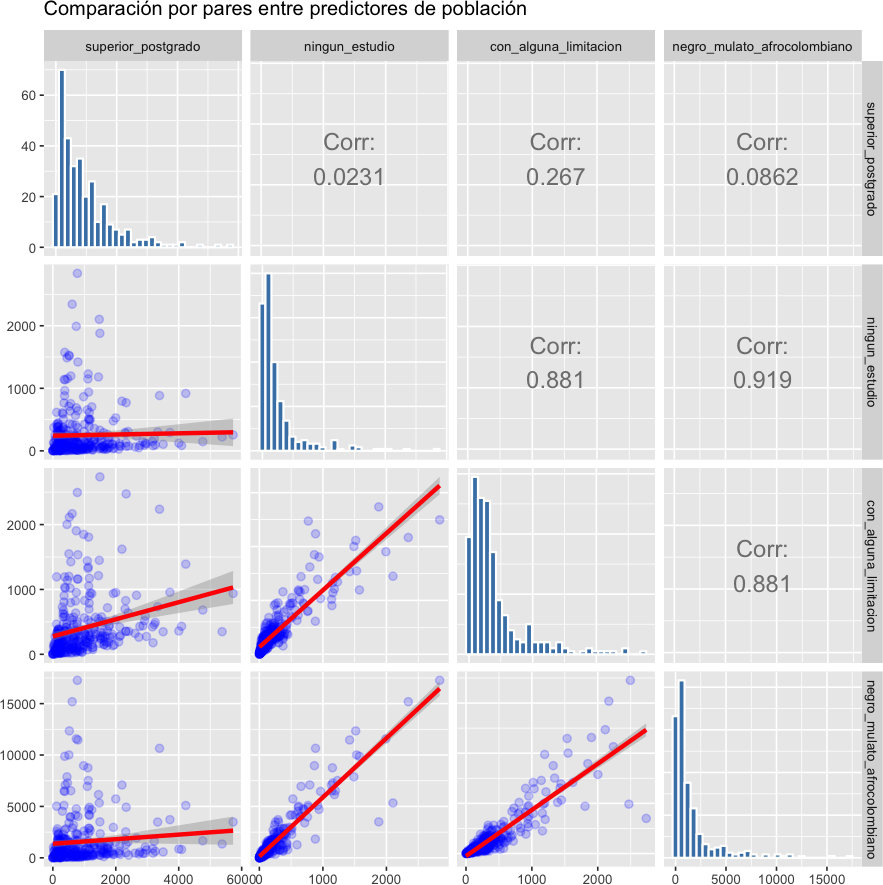
\includegraphics[width=1\linewidth]{tesis-unigis_files/figure-latex/bivar-poblacion-abs-1} 

}

\caption{Comparación por pares entre predictores de población}\label{fig:bivar-poblacion-abs}
\end{figure}

Las mismas variables expresadas como porcentaje de la población de un SU
muestran patrones similares (ver figura \ref{fig:bivar-poblacion-mod}):
existe una alta correlación negativa entre el porcentaje de población
afro de un sector y la tenencia de estudios superiores
(\(\simeq-0.71\)), una fuerte asociación positiva entre el porcentaje de
personas afro de un sector y el porcentaje de personas que carecen de
estudios (\(\simeq 0.68\)). También hay una fuerte relación inversa
entre el porcentaje de personas de un sector sin estudios y el
porcentaje de ellos que tiene estudios superiores (\(\simeq-0.8\)).
Estos resultados refuerzan la concentración de condiciones desfavorables
para la población explicadas por la condición racial.

\begin{figure}[H]

{\centering 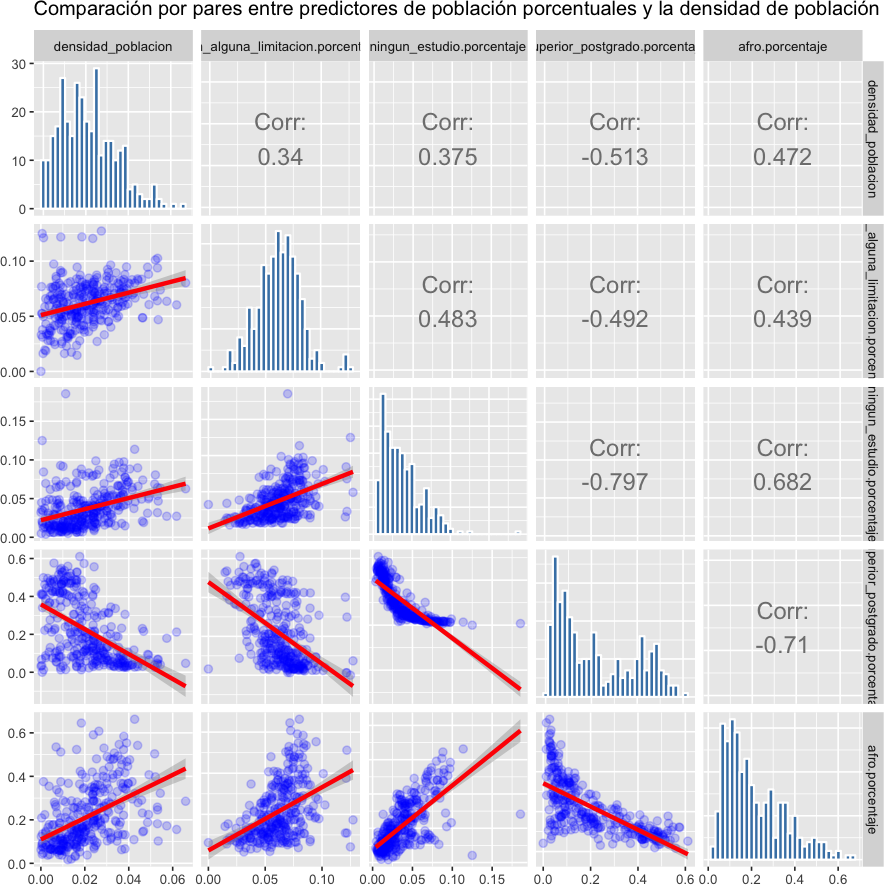
\includegraphics[width=1\linewidth]{tesis-unigis_files/figure-latex/bivar-poblacion-mod-1} 

}

\caption{Comparación por pares entre predictores de población porcentuales}\label{fig:bivar-poblacion-mod}
\end{figure}

Los gráficos de azulejos son una forma resumida para consultar la
intensidad de estas relaciones (figura \ref{fig:tile-poblacion-pearson})
lineales entre las variables dependientes usando el coeficiente de
correlación de Pearson, y las no lineales mediante el coeficiente de
Spearman (figura \ref{fig:tile-poblacion-spearman}).

Con base en los coeficientes de correlación de Pearson (figura
\ref{fig:tile-copa-poblacion-pearson}) y Spearman (figura
\ref{fig:tile-copa-poblacion-spearman}) entre las variables dependientes
e independientes, y teniendo en cuenta las restricciones de colinealidad
entre las variables dependientes, se seleccionaron las siguientes
variables para los modelos lineales:

\begin{itemize}
\item
  Para el área de copa (\texttt{area\_copa}) los predictores
  seleccionados son:
  \texttt{con\ estudios\ superiores,\ densidad\ de\ población,\ con\ alguna\ limitación\ {[}\%{]},\ afrocolombianos\ {[}\%{]}}.
\item
  Para la cobertura de copa (\texttt{cobertura\_copa.ap}) los
  predictores seleccionados son:
  \texttt{con\ estudios\ superiores\ {[}\%{]},\ densidad\ de\ población,\ con\ alguna\ limitación\ {[}\%{]},\ afrocolombianos\ {[}\%{]}}
\end{itemize}

Para la selección de variables sobre uso de los predios, los tipos de
vivienda y área de espacio público se aplicó el mismo proceso. Para el
área de copa se seleccionaron el área de espacios verdes y el porcentaje
de viviendas tipo cuarto. Para el modelo de porcentaje de cobertura se
seleccionaron el porcentaje de viviendas tipo apartamento, el porcentaje
de viviendas tipo cuarto y porcentaje de área de espacios verdes.

\begin{figure}[H]

{\centering 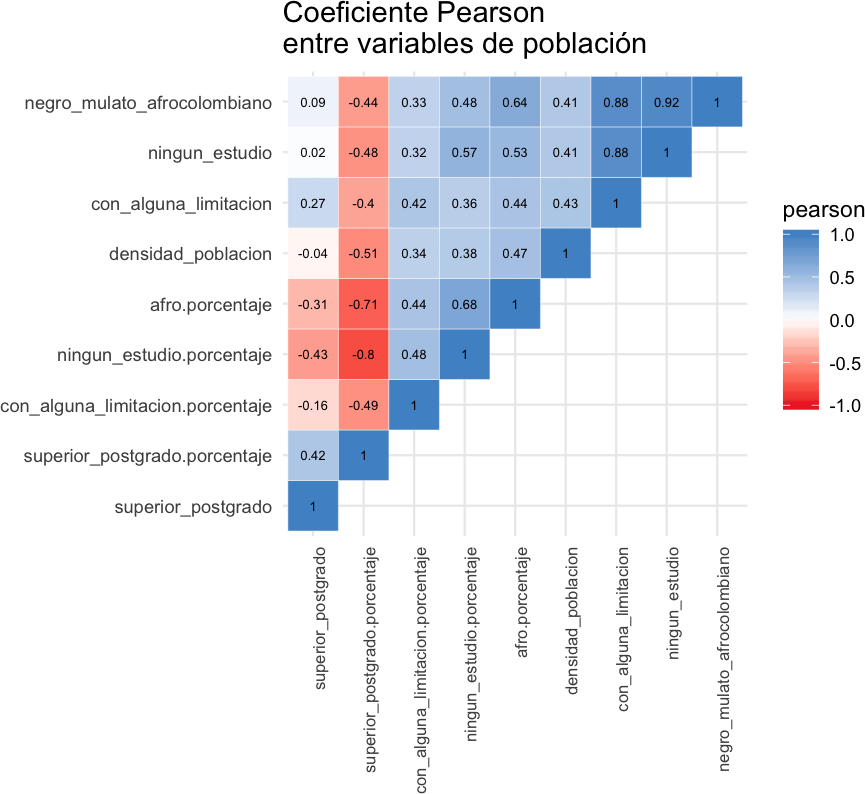
\includegraphics[width=1\linewidth]{tesis-unigis_files/figure-latex/tile-poblacion-pearson-1} 

}

\caption{Coeficiente Pearson entre variables de población}\label{fig:tile-poblacion-pearson}
\end{figure}

\begin{figure}[H]

{\centering 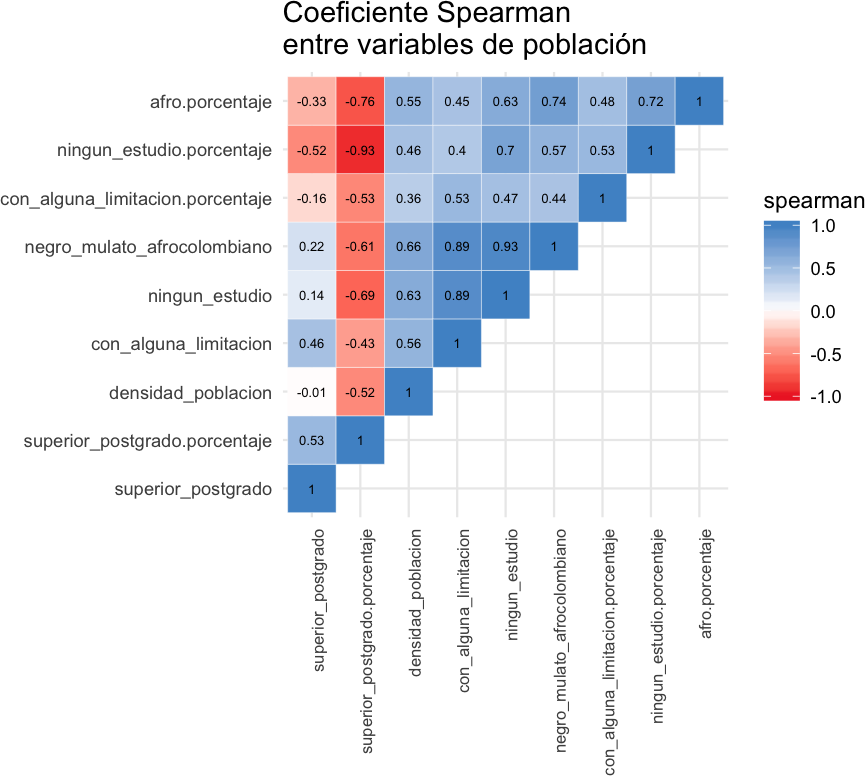
\includegraphics[width=1\linewidth]{tesis-unigis_files/figure-latex/tile-poblacion-spearman-1} 

}

\caption{Coeficiente Spearman entre variables de población}\label{fig:tile-poblacion-spearman}
\end{figure}

\begin{figure}[H]

{\centering 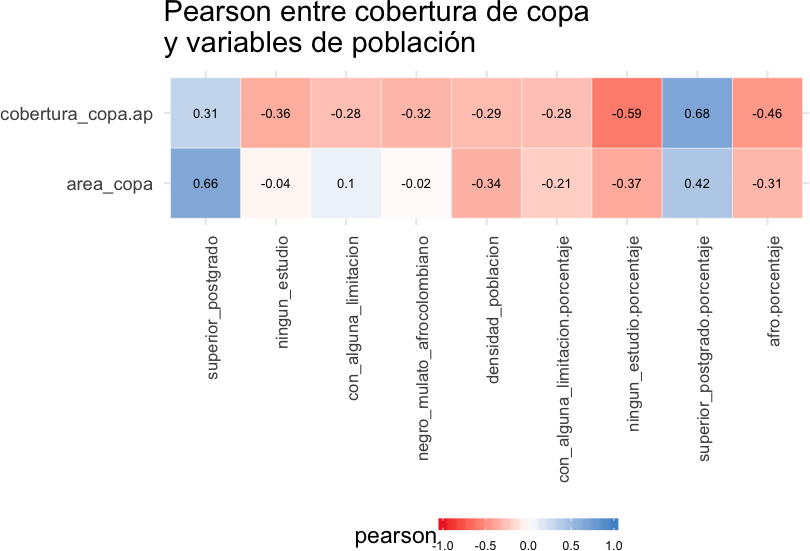
\includegraphics[width=1\linewidth]{tesis-unigis_files/figure-latex/tile-copa-poblacion-pearson-1} 

}

\caption{Coeficiente Pearson entre cobertura de copa y variables de población}\label{fig:tile-copa-poblacion-pearson}
\end{figure}

\begin{figure}[H]

{\centering 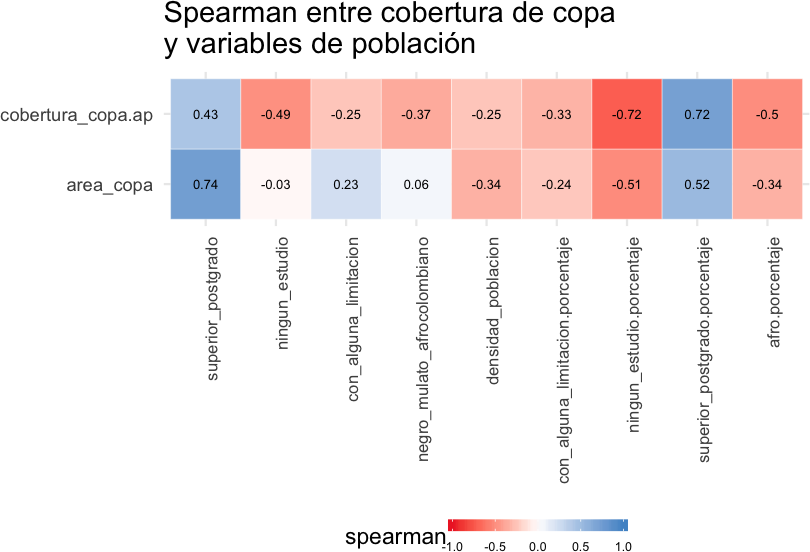
\includegraphics[width=1\linewidth]{tesis-unigis_files/figure-latex/tile-copa-poblacion-spearman-1} 

}

\caption{Coeficiente Spearman entre cobertura de copa y variables de población}\label{fig:tile-copa-poblacion-spearman}
\end{figure}

\subsection{Modelos de regresión lineal
AU}\label{modelos-de-regresiuxf3n-lineal-au}

Antes de evaluar los modelos se aplicaron varias transformaciones en
busca de normalizar las distribuciones de las variables dependientes.
Las que mejor resultado arrojaron en la formulación de los modelos
fueron la transformación logarítmica para el caso del área de copa y la
variable sin transformar en el caso de la cobertura de copa.

La tabla \ref{tab:coef-lm-copa} resume los coeficientes de la regresión
para el área de copa, la tabla \ref{tab:coef-lm-cobertura} resume los
coeficientes de la regresión para la cobertura de copa, y la tabla
\ref{tab:ajuste-lmcopa-pob-predios} resume las métricas de ajuste de
ambos modelos.

Los resultados de los test Shapiro-Wilk indican no normalidad en los
residuos en ambos modelos, heterocedasticidad como muestra el test
Breusch-Pagan y posibles no linealidades como se observa en las gráficas
diagnósticas de la regresión de ambos modelos( ver figuras
\ref{fig:diagn-mod-best-lm-copa} y \ref{fig:diagn-mod-best-lm-copaap}).

Sin embargo, el ajuste de ambos modelos tiene media de los residuos muy
cercanas a 0, al igual que el error cuadrático medio (MSE). En el caso
del área de copa se obtiene un \emph{adjR-square} de 60.5\%, que es
aceptable. Las variables significativas para el área de copa son:
\texttt{con\ estudios\ superiores}, \texttt{densidad\ de\ población},
\texttt{vivienda\ tipo\ cuarto\ {[}\%{]}}, \texttt{área\ de\ EV}. Los
resultados confirman que al nivel de toda el área de estudio, las
condiciones de acceso a la educación de la población, la densidad de
población, el tipo de vivienda y la disponibilidad de EV se correlaciona
con el acceso a servicios ambientales del AU.

Para la cobertura de copa la única variable significativa es
\texttt{con\ estudios\ superiores\ {[}\%{]}}. Este único indicador
porcentual, que hace una descripción local y comparable entre los SU,
explica el 45.9\% de la variabilidad de los datos, reforzando la
importancia del indicador de acceso a educación superior como predictor
del acceso a servicios ambientales del AU.

Para la siguientes fases se ignoraron las variables no significativas de
los modelos lineales.

\begin{table}[H]

\caption{\label{tab:coef-lm-copa}Coeficientes OLS de área de copa - Log(AC)}
\centering
\begin{tabular}{lrrrr}
\toprule
Término & Estimado & Error std. & t-valor & Pr(>|t|)\\
\midrule
Intercepto & 0.788 & 0.013 & 62.256 & 0.000\\
con estudios superiores & 0.312 & 0.024 & 13.013 & 0.000\\
densidad de población & -0.146 & 0.020 & -7.283 & 0.000\\
con alguna limitación [\%] & -0.020 & 0.025 & -0.813 & 0.417\\
afrocolombianos [\%] & 0.010 & 0.021 & 0.481 & 0.631\\
\addlinespace
vivienda tipo cuarto [\%] & -0.145 & 0.030 & -4.754 & 0.000\\
área de EV & 0.119 & 0.028 & 4.310 & 0.000\\
\bottomrule
\end{tabular}
\end{table}

\begin{table}[H]

\caption{\label{tab:coef-lm-cobertura}Coeficientes OLS de cobertura de copa - (CC)}
\centering
\begin{tabular}{lrrrr}
\toprule
Término & Estimado & Error std. & t-valor & Pr(>|t|)\\
\midrule
Intercepto & 0.03438 & 0.03989 & 0.86174 & 0.38948\\
con estudios superiores [\%] & 0.38210 & 0.04227 & 9.03961 & 0.00000\\
densidad de población & 0.05573 & 0.03750 & 1.48613 & 0.13824\\
con alguna limitación [\%] & 0.05848 & 0.04470 & 1.30827 & 0.19173\\
afrocolombianos [\%] & -0.02170 & 0.04410 & -0.49201 & 0.62306\\
\addlinespace
vivienda tipo apartamento [\%] & -0.04561 & 0.03547 & -1.28581 & 0.19945\\
vivienda tipo cuarto [\%] & -0.06197 & 0.06163 & -1.00545 & 0.31545\\
área de EV [\%] & 0.03971 & 0.03796 & 1.04619 & 0.29627\\
\bottomrule
\end{tabular}
\end{table}

\begin{table}[H]

\caption{\label{tab:ajuste-lmcopa-pob-predios}Resumen métricas de ajuste OLS para el área de copa (AC) y cobertura de copa (CC) }
\centering
\begin{tabular}{lrr}
\toprule
medidasfit & Log(AC) & \%CC\\
\midrule
Shapiro-Wilk & 0.98196 & 0.90416\\
SW p-value & 0.00043 & 0.00000\\
Breusch-Pagan & 21.62587 & 19.67634\\
BP p-value & 0.00142 & 0.00631\\
Media Residuos & 0.00000 & 0.00000\\
\addlinespace
MSE & 0.00345 & 0.01071\\
adj-Rsquare & 0.60479 & 0.45931\\
AIC & -901.82032 & -532.26094\\
Log likelihood & 458.91016 & 275.13047\\
\bottomrule
\end{tabular}
\end{table}

\begin{figure}[H]

{\centering 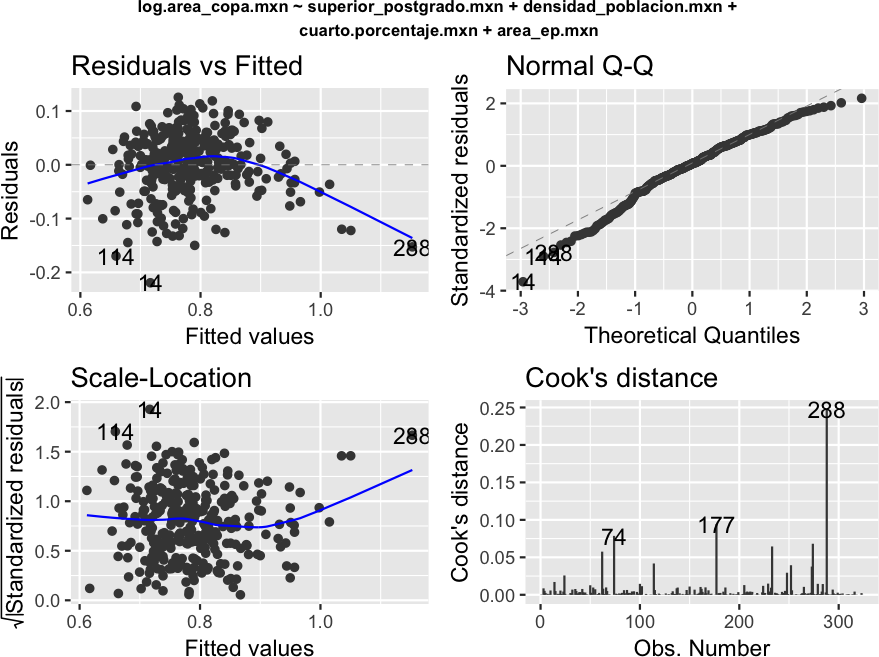
\includegraphics[width=1\linewidth]{tesis-unigis_files/figure-latex/diagn-mod-best-lm-copa-1} 

}

\caption{Gráficas diagnósticas para el análisis de regresión lineal de área de copa}\label{fig:diagn-mod-best-lm-copa}
\end{figure}

\begin{figure}[H]

{\centering 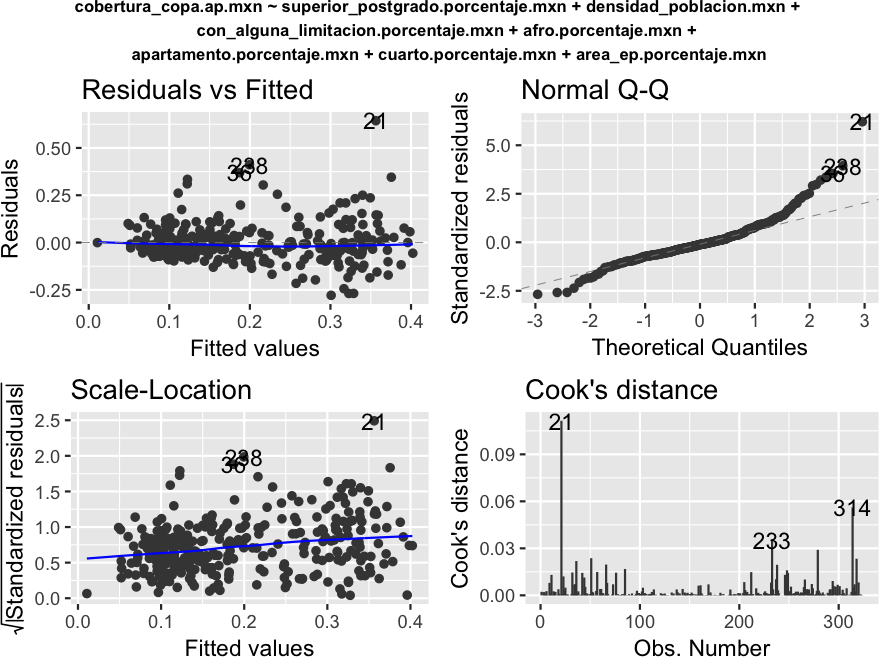
\includegraphics[width=1\linewidth]{tesis-unigis_files/figure-latex/diagn-mod-best-lm-copaap-1} 

}

\caption{Gráficas diagnósticas para el análisis de regresión lineal de porcentaje de cobertura de copa}\label{fig:diagn-mod-best-lm-copaap}
\end{figure}

\subsection{Modelado espacial AU}\label{modelado-espacial-au}

Las matrices de vecindad construidas para el análisis espacial son la
\emph{queen} \(W_q\), que considera vecino a todos los sectores que
comparten un lado o una esquina con un SU; y una matriz de distancia
inversas entre los centroides de los SU, restringiendo la vecindad a
aquellos centroides que están a menos de 1 km (\(W_d\)). El valor de un
kilómetro es arbitrario, aunque razonable en la escala humana. Los
grafos que representan las 2 matrices \(W\) se muestran en la figura
\ref{fig:ws-su-reg}.

\begin{figure}[H]

{\centering 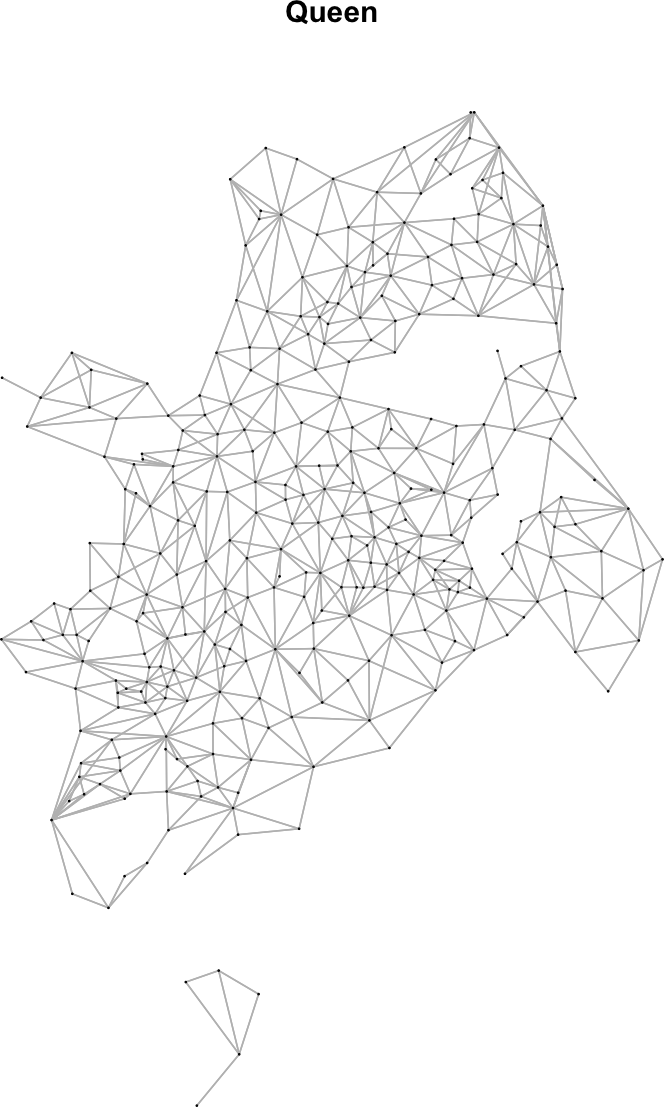
\includegraphics[width=0.48\linewidth]{tesis-unigis_files/figure-latex/ws-su-reg-1} 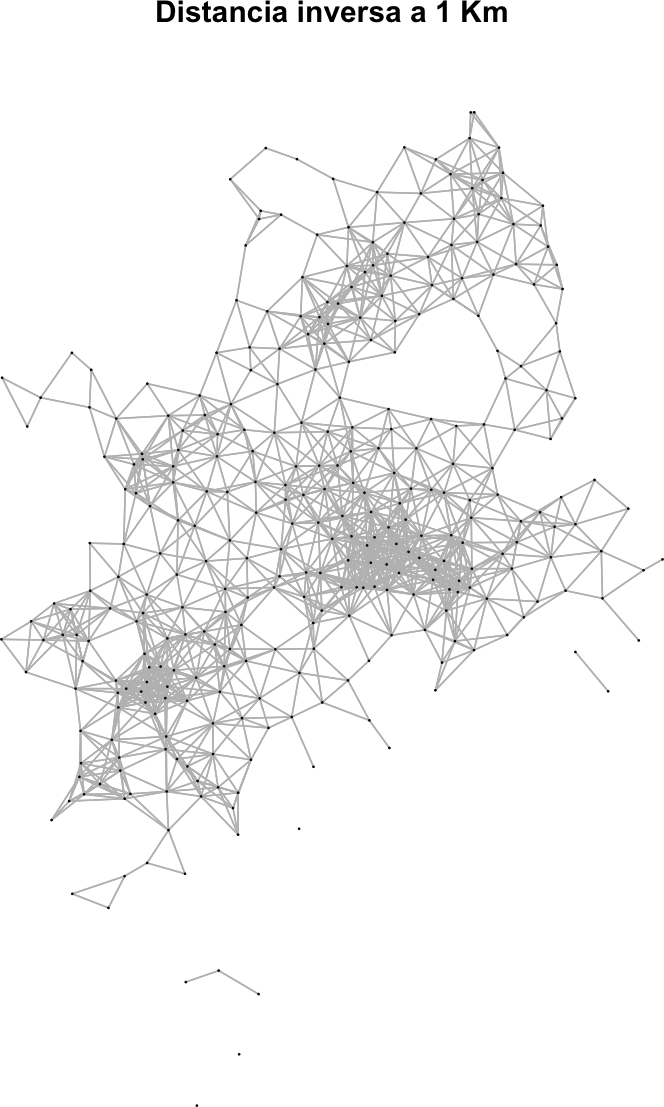
\includegraphics[width=0.48\linewidth]{tesis-unigis_files/figure-latex/ws-su-reg-2} 

}

\caption{Matrices de vecindad del análisis espacial}\label{fig:ws-su-reg}
\end{figure}

\subsubsection{Autocorrelación variables
dependientes}\label{autocorrelaciuxf3n-variables-dependientes}

Se analizó la autocorrelación de las variables dependientes para
encontrar agrupaciones existentes en los datos que pueden ser explicados
por la estructura de vecindad. Los resultados de los test de Moran'I
para ambas variables dependientes muestran que existen patrones de
agrupamiento y que puede rechazarse la hipótesis nula de que los
procesos espaciales subyacentes son aleatorios (ver tablas
\ref{tab:moran-copa-w} y \ref{tab:moran-copaap-w}).

Ambos diseños de matriz revelan presencia clara de autocorrelación
espacial. La matriz \(W_q\) captura mejor la autocorrelación del área de
copa. En el caso de la cobertura de copa la matriz \(W_d\) presenta un
valor ligeramente mayor de autocorrelación.

Los mapas LISA muestran los grupos de sectores que configuran la
autocorrelación del área de copa usando la matriz para \(W_q\) (figura
\ref{fig:mapas-lisa-copa-wq}) y los grupos de la variable cobertura de
copa usando la matriz \(W_d\) (figura \ref{fig:mapas-lisa-copaap-wd}).

Los grupos que se forman muestran patrones distintos en los dos
indicadores seleccionados para caracterizar los beneficios del arbolado
urbano. Sin embargo, existen SU comunes en los grupos conformados pero
con diferencias en la extensión de los conglomerados identificados. Esto
se debe a que cada uno de los indicadores expresa un concepto distinto
del disfrute de ese beneficio: el área de copa muestra las diferencias
desde una perspectiva global, es decir, con base en el valor absoluto de
área de copa de un SU en relación al total de área disponible en toda la
ciudad. El indicador de cobertura de copa expresa el beneficio de forma
relativa entre los SU al dividir el área de copa disponible en un SU
entre el área pública de ese SU.

Es clara la similitud entre los grupos obtenidos para una misma variable
dependiente con ambos diseños de matriz \(W\) (figura
\ref{fig:mapas-lisa-copa-wq} y figura \ref{fig:mapas-lisa-copa-wd} para
el área de copa y \ref{fig:mapas-lisa-copaap-wq} y
\ref{fig:mapas-lisa-copaap-wd} para la cobertura de copa), posiblemente
porque no existen diferencias notables entre los dos tipos de estructura
de vecindad propuestas (figura \ref{fig:ws-su-reg}).

\begin{table}[H]

\caption{\label{tab:moran-copa-w}Test de Moran - Área de copa para $W_q$ y $W_d$}
\centering
\begin{tabular}{lrr}
\toprule
  & $W_q$ & $W_d$\\
\midrule
Estadístico Moran I & 0.37488 & 0.28174\\
Expectativa & -0.00310 & -0.00312\\
Varianza & 0.00119 & 0.00090\\
Desviación estándar de Moran I & 10.95802 & 9.50984\\
p-valor & 0.00000 & 0.00000\\
\bottomrule
\end{tabular}
\end{table}

\begin{table}[H]

\caption{\label{tab:moran-copaap-w}Test de Moran - Porcentaje de cobertura de copa para $W_q$ y $W_d$}
\centering
\begin{tabular}{lrr}
\toprule
  & $W_q$ & $W_d$\\
\midrule
Estadístico Moran I & 0.48104 & 0.50225\\
Expectativa & -0.00310 & -0.00312\\
Varianza & 0.00118 & 0.00089\\
Desviación estándar de Moran I & 14.10670 & 16.95747\\
p-valor & 0.00000 & 0.00000\\
\bottomrule
\end{tabular}
\end{table}

\begin{figure}[H]

{\centering 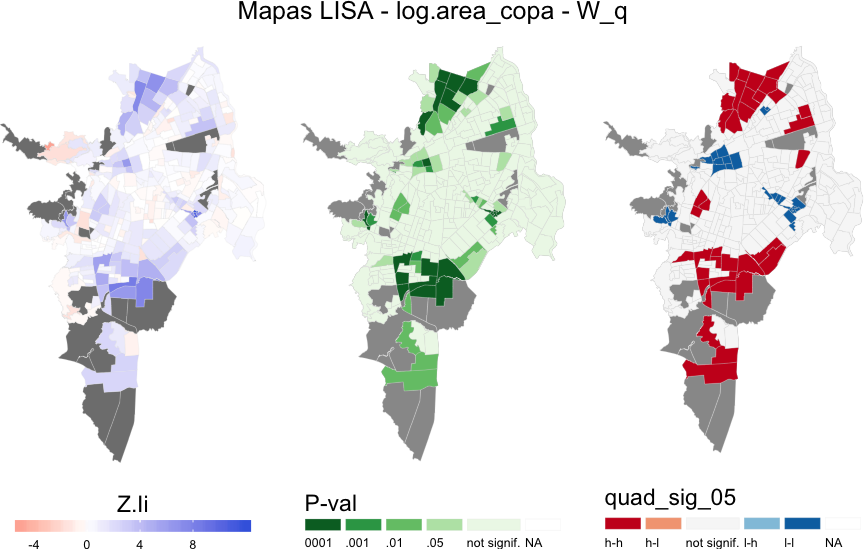
\includegraphics[width=1\linewidth]{tesis-unigis_files/figure-latex/mapas-lisa-copa-wq-1} 

}

\caption{Mapas LISA para la matriz $W_q$ del indicador área de copa}\label{fig:mapas-lisa-copa-wq}
\end{figure}

\begin{figure}[H]

{\centering 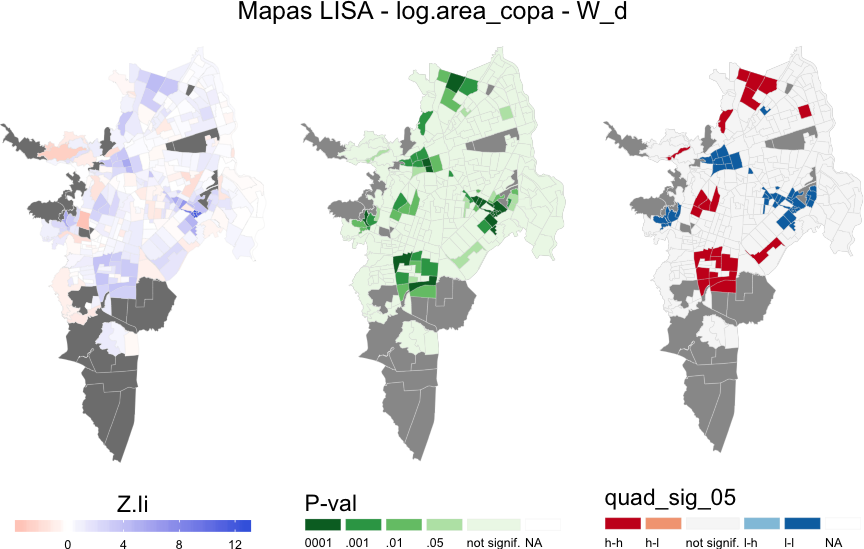
\includegraphics[width=1\linewidth]{tesis-unigis_files/figure-latex/mapas-lisa-copa-wd-1} 

}

\caption{Mapas LISA para la matriz $W_d$ del indicador área de copa}\label{fig:mapas-lisa-copa-wd}
\end{figure}

\begin{figure}[H]

{\centering 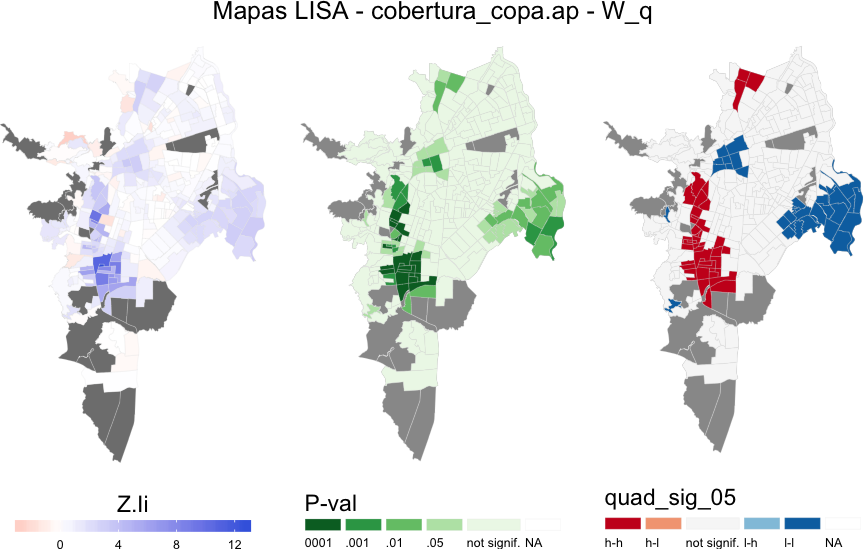
\includegraphics[width=1\linewidth]{tesis-unigis_files/figure-latex/mapas-lisa-copaap-wq-1} 

}

\caption{Mapas LISA para la matriz $W_q$ del indicador cobertura de copa}\label{fig:mapas-lisa-copaap-wq}
\end{figure}

\begin{figure}[H]

{\centering 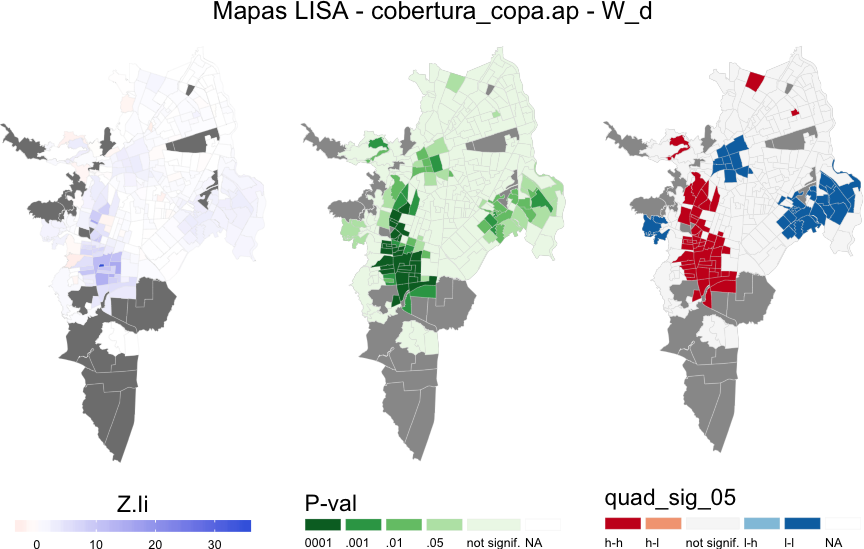
\includegraphics[width=1\linewidth]{tesis-unigis_files/figure-latex/mapas-lisa-copaap-wd-1} 

}

\caption{Mapas LISA para la matriz $W_d$ de del indicador cobertura de copa}\label{fig:mapas-lisa-copaap-wd}
\end{figure}

\subsubsection{Autocorrelación residuos de los
OLS}\label{autocorrelaciuxf3n-residuos-de-los-ols}

Para evaluar la utilidad de aplicar modelos espaciales de regresión se
examinó la existencia de autocorrelación en los residuos de los modelos
de regresión lineal. Se comparó si alguno de las estructuras de vecindad
produce resultados significativamente mejores en la detección de
autocorrelación espacial.

La tabla \ref{tab:moran-rescopa-w} muestra ambos diseños de matriz \(W\)
presentan un valor de Moran Global mayor que 0 y significativo para los
residuos del OLS de área de copa, al igual que para los residuos del OLS
del porcentaje de cobertura (ver tabla \ref{tab:moran-rescopaap-w}).

En ambos modelos el resultado de autocorrelación espacial sugiere que al
introducir retardos espaciales y la estructura de vecindad pueden
mejorar la estimación de los coeficientes de la regresión y las métricas
de desempeño del ajuste.

\begin{table}[H]

\caption{\label{tab:moran-rescopa-w}Test de Moran - Residuos de OLS Área de copa para $W_q$ y $W_d$}
\centering
\begin{tabular}{lrr}
\toprule
  & $W_q$ & $W_d$\\
\midrule
Estadístico Moran I & 0.09660 & 0.11579\\
Expectativa & -0.00310 & -0.00312\\
Varianza & 0.00119 & 0.00090\\
Desviación estándar de Moran I & 2.89161 & 3.97182\\
p-valor & 0.00192 & 0.00004\\
\bottomrule
\end{tabular}
\end{table}

\begin{table}[H]

\caption{\label{tab:moran-rescopaap-w}Test de Moran - Residuos de OLS Porcentaje de cobertura de copa para $W_q$ y $W_d$}
\centering
\begin{tabular}{lrr}
\toprule
  & $W_q$ & $W_d$\\
\midrule
Estadístico Moran I & 0.19436 & 0.18821\\
Expectativa & -0.00310 & -0.00312\\
Varianza & 0.00117 & 0.00088\\
Desviación estándar de Moran I & 5.78107 & 6.45120\\
p-valor & 0.00000 & 0.00000\\
\bottomrule
\end{tabular}
\end{table}

\subsubsection{Modelo espacial área de
copa}\label{modelo-espacial-uxe1rea-de-copa}

Las métricas de ajuste de los modelos con las matrices de vecindad
\(W_d\) (ver tabla \ref{tab:tabla-comp-modelos-copa-wd}) y \(W_q\)
(tabla \ref{tab:tabla-comp-modelos-copa-wq}) para el área de copa
muestran que los modelos espaciales logran eliminar la autocorrelación
espacial global en los residuos. Es importante anotar que la
heterocedasticidad reportada en la tabla
\ref{tab:ajuste-lmcopa-pob-predios} del modelo OLS desaparece al
descartar las variables independientes con \(p\)-valores no
significativos, por lo que no se le puede adjudicar al uso de los
términos espaciales. Todos los modelos mejoran las métricas de error
respecto del OLS y ninguno logra la normalidad en los residuos, aunque
en las gráficas diagnósticas se aprecia una semblanza aceptable (ver
figura \ref{fig:diag-model-espaciales}) con problemas en valores
extremos.

Al comparar los resultados usando el desempeño en criterio de
información de Akaike (AIC), el mejor fue el SEM con la matriz \(W_d\),
seguido del SD con \(W_q\), con leves diferencias entre las métricas. En
cuanto a \(\lambda\) (tabla \ref{tab:cauto-sem-copa}) y \(\rho\) (tabla
\ref{tab:cauto-sd-copa-wq}) , los términos autorregresivos, son
significativos para SEM \(W_d\) y para SD con \(W_q\) respectivamente.

El resultado del modelo SEM confirma la significancia de las variables
de cantidad de personas con estudios superiores y porcentaje de espacio
verde, con coeficientes de valores positivos, en ese orden de
importancia. La densidad de población y la presencia de viviendas tipo
cuarto, con coeficientes negativos, son factores que disminuyen la
disponibilidad de área de copa en un SU (ver tabla
\ref{tab:coef-sem-copa-wd}). Existen cambios y ajustes en los valores de
los coeficientes con relación al modelo OLS, que dadas las mejoras en
las métricas de ajuste hacen más confiables las estimaciones.

\begin{table}[H]

\caption{\label{tab:tabla-comp-modelos-copa-wq}Metricas de ajuste para los modelos de área de copa $W_q$}
\centering
\begin{tabular}{lrrrr}
\toprule
medidasfit & OLS & SAR & SEM & SD\\
\midrule
Globla Moran'I & 0.09660 & -0.01056 & -0.01056 & -0.00157\\
GMI p-value & 0.00192 & 0.58578 & 0.58574 & 0.48239\\
Shapiro-Wilk & 0.97939 & 0.97959 & 0.97638 & 0.98307\\
SW p-value & 0.00013 & 0.00015 & 0.00004 & 0.00073\\
Breusch-Pagan & 6.70653 & 4.36429 & 5.08935 & 10.28094\\
\addlinespace
BP p-value & 0.15223 & 0.35894 & 0.27825 & 0.24586\\
Media Residuos & 0.00000 & 0.00000 & 0.00000 & 0.00000\\
MSE & 0.00345 & 0.00330 & 0.00335 & 0.00322\\
adj-Rsquare & 0.60639 & NA & NA & NA\\
Nagelkerke pseudo-R-squared & NA & 0.62529 & 0.61948 & 0.63462\\
\addlinespace
AIC & -905.09560 & -914.99865 & -910.01741 & -915.17149\\
Log likelihood & 458.54780 & 464.49933 & 462.00870 & 468.58574\\
\bottomrule
\end{tabular}
\end{table}

\begin{table}[H]

\caption{\label{tab:tabla-comp-modelos-copa-wd}Metricas de ajuste para los modelos de área de copa con $W_d$}
\centering
\begin{tabular}{lrrrr}
\toprule
medidasfit & OLS & SAR & SEM & SD\\
\midrule
Globla Moran'I & 0.11579 & 0.08293 & -0.01362 & 0.07133\\
GMI p-value & 0.00004 & 0.00202 & 0.63708 & 0.00645\\
Shapiro-Wilk & 0.97939 & 0.98468 & 0.97628 & 0.98522\\
SW p-value & 0.00013 & 0.00160 & 0.00003 & 0.00210\\
Breusch-Pagan & 6.70653 & 8.80615 & 5.51317 & 11.99026\\
\addlinespace
BP p-value & 0.15223 & 0.06613 & 0.23857 & 0.15164\\
Media Residuos & 0.00000 & 0.00000 & -0.00001 & 0.00000\\
MSE & 0.00345 & 0.00340 & 0.00327 & 0.00333\\
adj-Rsquare & 0.60639 & NA & NA & NA\\
Nagelkerke pseudo-R-squared & NA & 0.61640 & 0.62586 & 0.62438\\
\addlinespace
AIC & -905.09560 & -907.40643 & -915.49806 & -906.21535\\
Log likelihood & 458.54780 & 460.70321 & 464.74903 & 464.10768\\
\bottomrule
\end{tabular}
\end{table}

\begin{figure}[H]

{\centering 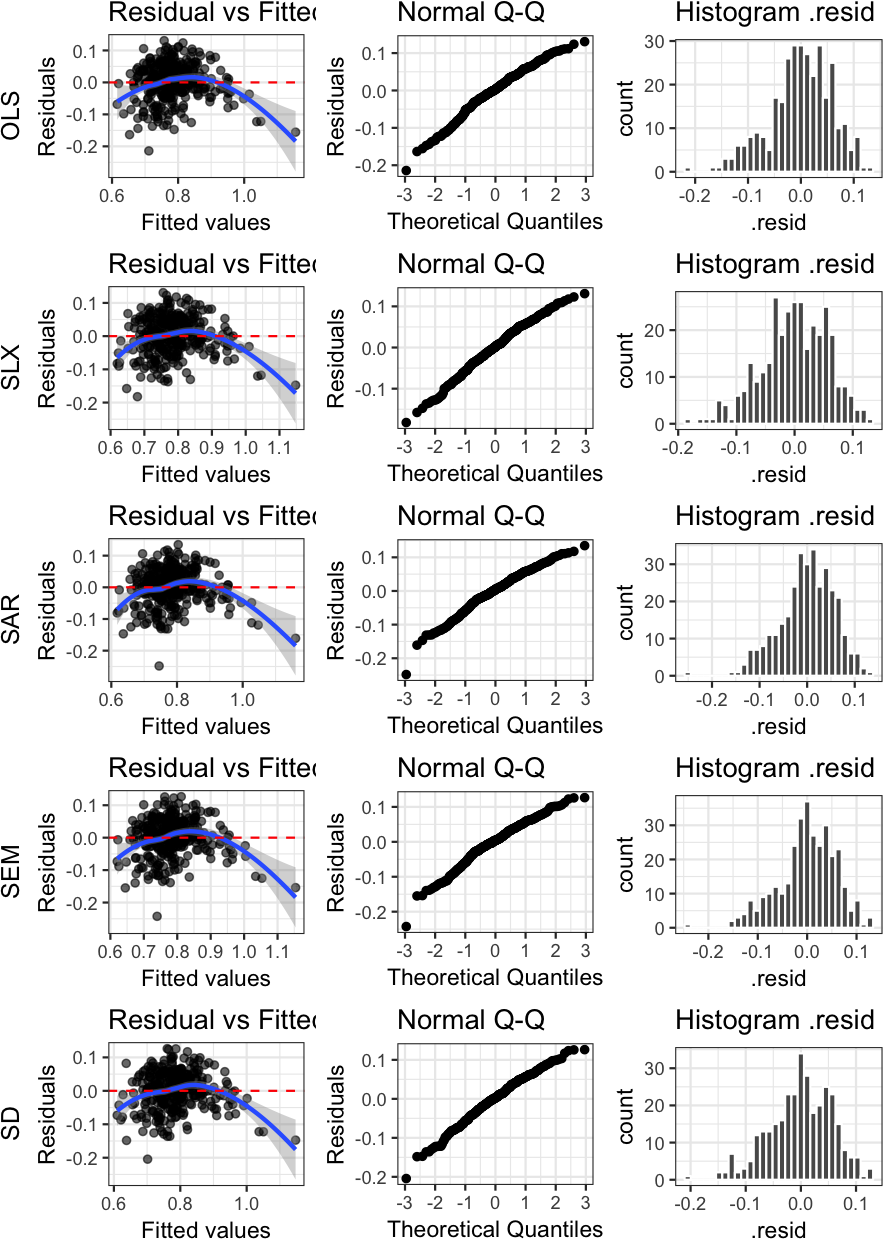
\includegraphics[width=1\linewidth]{tesis-unigis_files/figure-latex/diag-model-espaciales-1} 

}

\caption{Diagnóstico comparativo entre modelos espaciales de área de copa}\label{fig:diag-model-espaciales}
\end{figure}

\begin{table}[H]

\caption{\label{tab:coef-sem-copa-wd}Coeficientes del modelo SEM de área de copa $W_d$}
\centering
\begin{tabular}{lrrrr}
\toprule
Término & Estimado & Error std. & t-valor & Pr(>|t|)\\
\midrule
Intercepto & 0.779 & 0.009 & 83.105 & 0\\
con estudios superiores & 0.299 & 0.023 & 13.154 & 0\\
densidad de población & -0.140 & 0.019 & -7.359 & 0\\
vivienda tipo cuarto [\%] & -0.132 & 0.032 & -4.168 & 0\\
área de EV & 0.133 & 0.027 & 4.871 & 0\\
\bottomrule
\end{tabular}
\end{table}

\begin{table}[H]

\caption{\label{tab:cauto-sem-copa}Coeficiente de autocorrelación modelo SEM de área de copa $W_d$}
\centering
\begin{tabular}{lll}
\toprule
$\lambda$ & Likelihood ratio & p-valor\\
0.316 & 12.402 & 0\\
\bottomrule
\end{tabular}
\end{table}

\begin{table}[H]

\caption{\label{tab:coef-sd-copa-wq}Coeficientes del modelo SD de área de copa $W_q$}
\centering
\begin{tabular}{lrrrr}
\toprule
Término & Estimado & Error std. & t-valor & Pr(>|t|)\\
\midrule
Intercepto & 0.637 & 0.065 & 9.828 & 0.000\\
con estudios superiores & 0.287 & 0.024 & 12.023 & 0.000\\
densidad de población & -0.096 & 0.025 & -3.783 & 0.000\\
vivienda tipo cuarto [\%] & -0.059 & 0.041 & -1.438 & 0.151\\
área de EV & 0.141 & 0.030 & 4.689 & 0.000\\
\addlinespace
estudios superiores (retardada) & -0.016 & 0.047 & -0.331 & 0.741\\
densidad de población (retardada) & -0.050 & 0.037 & -1.356 & 0.175\\
vivienda tipo cuarto [\%] (retardada) & -0.146 & 0.065 & -2.226 & 0.026\\
área de EV (retardada) & -0.074 & 0.040 & -1.832 & 0.067\\
\bottomrule
\end{tabular}
\end{table}

\begin{table}[H]

\caption{\label{tab:cauto-sd-copa-wq}Coeficiente de autocorrelación modelo SD de área de copa $W_q$}
\centering
\begin{tabular}{lll}
\toprule
$\rho$ & Likelihood ratio & p-valor\\
0.201 & 6.415 & 0.011\\
\bottomrule
\end{tabular}
\end{table}

\subsubsection{Modelo espacial porcentaje de cobertura de área de
copa}\label{modelo-espacial-porcentaje-de-cobertura-de-uxe1rea-de-copa}

Las métricas de ajuste de los modelos con las matrices de vecindad
\(W_d\) (ver tabla \ref{tab:tabla-comp-modelos-copaap-wd}) y \(W_q\)
(tabla \ref{tab:tabla-comp-modelos-copaap-wq}) para el porcentaje de
cobertura de copa muestran que los modelos espaciales logran eliminar la
autocorrelación espacial global en los residuos, excepto el SAR con
\(W_d\). Todos los modelos mejoran las métricas de error con respecto al
OLS y ninguno logra la normalidad en los residuos ni eliminar la
heterocedasticidad como se aprecia en las gráficas diagnósticas (ver
figura \ref{fig:diag-model-espaciales-copaap}).

Al comparar los resultados usando el desempeño en AIC, el mejor fue el
SD con la matriz \(W_d\). \(\rho\), el término autorregresivo, es de un
valor alto y muy significativo para el modelo SD con \(W_d\) (tabla
\ref{tab:cauto-sd-copaap-wd}).

El resultado del modelo SD confirma la significancia de la única
variable independiente: porcentaje de personas con estudios superiores,
con coeficiente positivo, identificándolo como un factores relacionado
con alta proporción de área de copa en un SU (ver tabla
\ref{tab:coef-sd-copaap}). Existen una reducción del valor del
coeficiente con relación al modelo OLS.

La variable de \textbf{estudios superiores} en la población refleja el
patrón de agrupamiento espacial de la cobertura de copa pero es poco
significativa como variable retardada, cuestión que pone dudas sobre si
el SD proponga una interpretación acertada o diferente de un modelo
autorregresivo puro (SAR).

\begin{table}[H]

\caption{\label{tab:tabla-comp-modelos-copaap-wq}Metricas de ajuste para los modelos de porcentaje de área de copa $W_q$}
\centering
\begin{tabular}{lrrrr}
\toprule
medidasfit & OLS & SAR & SEM & SD\\
\midrule
Globla Moran'I & 0.19436 & 0.00734 & -0.01131 & -0.00863\\
GMI p-value & 0.00000 & 0.37996 & 0.59509 & 0.56441\\
Shapiro-Wilk & 0.90492 & 0.89936 & 0.89238 & 0.89685\\
SW p-value & 0.00000 & 0.00000 & 0.00000 & 0.00000\\
Breusch-Pagan & 16.82734 & 16.22458 & 15.21537 & 17.19946\\
\addlinespace
BP p-value & 0.00004 & 0.00006 & 0.00010 & 0.00018\\
Media Residuos & 0.00000 & 0.00000 & 0.00000 & 0.00000\\
MSE & 0.01100 & 0.00979 & 0.00981 & 0.00972\\
adj-Rsquare & 0.45512 & NA & NA & NA\\
Nagelkerke pseudo-R-squared & NA & 0.50267 & 0.49988 & 0.50390\\
\addlinespace
AIC & -535.66434 & -562.24323 & -560.43438 & -561.04776\\
Log likelihood & 270.83217 & 285.12162 & 284.21719 & 285.52388\\
\bottomrule
\end{tabular}
\end{table}

\begin{table}[H]

\caption{\label{tab:tabla-comp-modelos-copaap-wd}Metricas de ajuste para los modelos de porcentaje de área de copa $W_d$}
\centering
\begin{tabular}{lrrrr}
\toprule
medidasfit & OLS & SAR & SEM & SD\\
\midrule
Globla Moran'I & 0.18821 & 0.07353 & 0.00335 & 0.01940\\
GMI p-value & 0.00000 & 0.00487 & 0.41351 & 0.22373\\
Shapiro-Wilk & 0.90492 & 0.89936 & 0.88316 & 0.90138\\
SW p-value & 0.00000 & 0.00000 & 0.00000 & 0.00000\\
Breusch-Pagan & 16.82734 & 16.22458 & 10.35903 & 17.66672\\
\addlinespace
BP p-value & 0.00004 & 0.00006 & 0.00129 & 0.00015\\
Media Residuos & 0.00000 & 0.00000 & 0.00017 & 0.00000\\
MSE & 0.01100 & 0.00979 & 0.00950 & 0.00931\\
adj-Rsquare & 0.45512 & NA & NA & NA\\
Nagelkerke pseudo-R-squared & NA & 0.50267 & 0.51018 & 0.52395\\
\addlinespace
AIC & -535.66434 & -562.24323 & -567.17585 & -574.41489\\
Log likelihood & 270.83217 & 285.12162 & 287.58793 & 292.20744\\
\bottomrule
\end{tabular}
\end{table}

\begin{figure}[H]

{\centering 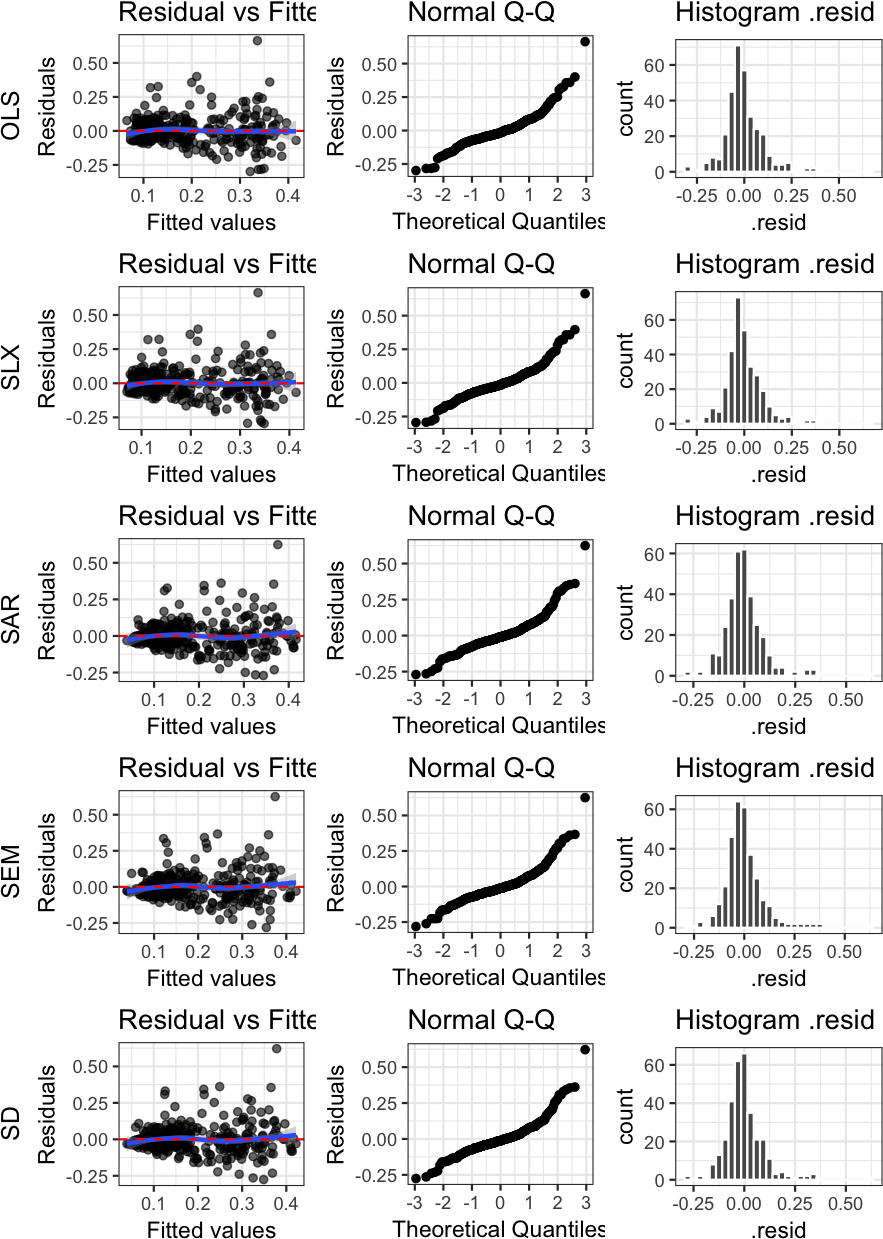
\includegraphics[width=1\linewidth]{tesis-unigis_files/figure-latex/diag-model-espaciales-copaap-1} 

}

\caption{Diagnóstico comparativo entre modelos de porcentaje de copa}\label{fig:diag-model-espaciales-copaap}
\end{figure}

\begin{table}[H]

\caption{\label{tab:cauto-sd-copaap-wd}Coeficiente de autocorrelación modelo SD $W_d$ de porcentaje de área de copa }
\centering
\begin{tabular}{lll}
\toprule
$\rho$ & Likelihood ratio & p-valor\\
0.465 & 32.069 & 0\\
\bottomrule
\end{tabular}
\end{table}

\begin{table}[H]

\caption{\label{tab:coef-sd-copaap}Coeficientes del modelo SD de porcentaje de área de copa $W_d$}
\centering
\begin{tabular}{lrrrr}
\toprule
Término & Estimado & Error std. & t-valor & Pr(>|t|)\\
\midrule
Intercepto & 0.023 & 0.011 & 2.206 & 0.027\\
con estudios superiores [\%] & 0.239 & 0.034 & 6.941 & 0.000\\
estudios superiores [\%] (retardada) & -0.021 & 0.050 & -0.407 & 0.684\\
\bottomrule
\end{tabular}
\end{table}

\section{Acceso a espacios verdes}\label{acceso-a-espacios-verdes-1}

En el caso de los EV la literatura ofrece variedad de medidas sobre
acceso en relación con la distancia o con el área disponible. Se
eligieron dos métricas: el porcentaje de área de espacio verde de un
sector censal, para cuantificar beneficios a nivel local; y la razón
área disponible entre distancia (\texttt{ia.areas.dist}) (ecuación
\eqref{eq:areas-dists}) que expresa el acceso más allá de los límites del
SU. El valor es cercano a cero cuando el área disponible es cercana a
cero o cuando la distancia es mucho mayor que el área media de espacio
verde en el radio de búsqueda, limitado a 1000 \(m\), un orden de
magnitud menor que el área media de EV (22,971.4 \(m^2\)). La distancia
promedio del centroide de un SU al conjunto de EV es 644.7 \(m\). Como
se observa en la figura \ref{fig:mapa-dependienteEV-sel}, esta medición
parece un versión interpolada del indicador local de acceso porcentaje
de área de EV (\texttt{area\_ep.porcentaje}), y hace evidente un patrón
espacial de grupos con mejor acceso a EV, no uniforme ni aleatorio.

Al examinar la distribución de los valores de estos indicadores (figuras
\ref{fig:hist-areaep} y \ref{fig:hist-areasdist}) se observa que en
ambos indicadores existe asimetría positiva, lo que muestra una
concentración de valores por debajo del promedio del indicador y un
conjunto reducido de SU muy por encima.

\begin{figure}[H]

{\centering 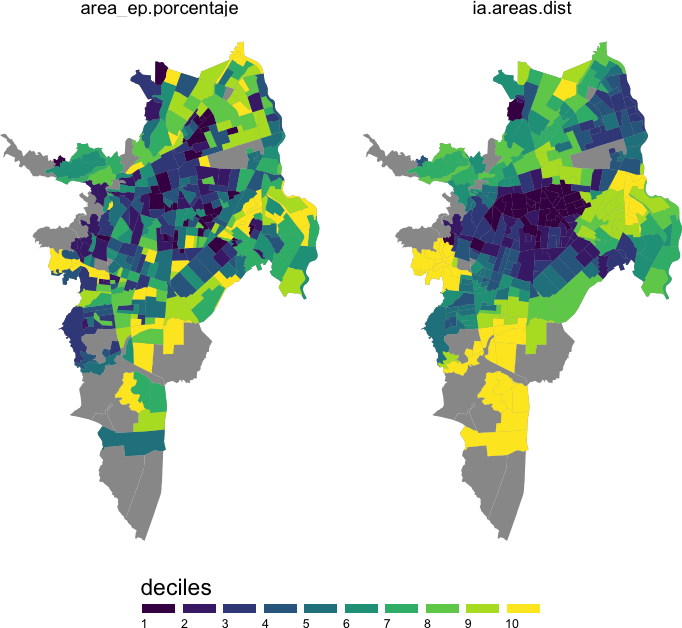
\includegraphics[width=0.8\linewidth]{tesis-unigis_files/figure-latex/mapa-dependienteEV-sel-1} 

}

\caption{Métricas de acceso a espacio verdes seleccionadas}\label{fig:mapa-dependienteEV-sel}
\end{figure}

\begin{figure}[H]

{\centering 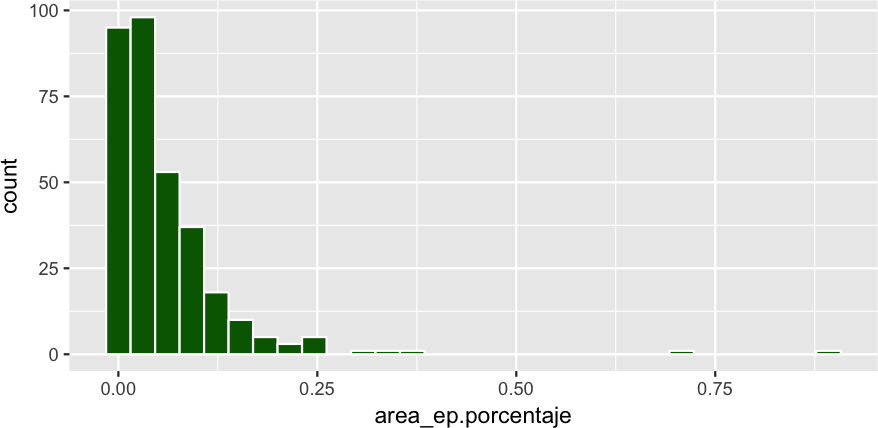
\includegraphics[width=1\linewidth]{tesis-unigis_files/figure-latex/hist-areaep-1} 

}

\caption{Distribucion del indicador de acceso local a EV }\label{fig:hist-areaep}
\end{figure}

\begin{figure}[H]

{\centering 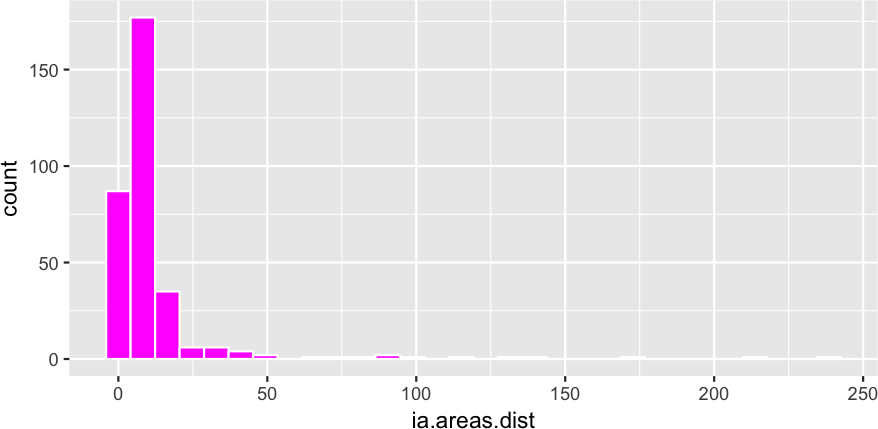
\includegraphics[width=1\linewidth]{tesis-unigis_files/figure-latex/hist-areasdist-1} 

}

\caption{Distribucion del indicador de acceso a EV área-distancia }\label{fig:hist-areasdist}
\end{figure}

\subsection{Correlaciones y distribuciones
bivariadas}\label{correlaciones-y-distribuciones-bivariadas}

Las figuras \ref{fig:tile-ev-poblacion-pearson} y
\ref{fig:tile-ev-poblacion-spearman} resumen los resultados del cálculo
de los coeficientes de Pearson y Spearman respectivamente de las
variables poblacionales y los indicadores de acceso. Esta relación es
muy débil, y en todas las variables (y para ambos coeficientes de
correlación) es inferior a 0.3, un valor considerado bajo para
seleccionar una variable como candidata a predictor de una regresión
lineal. Sin embargo, como parte del proceso para indagar sobre el efecto
en la estimación de parámetros de los modelos geoestadísticos, se
incluyeron las de mejor correlación: \texttt{densidad\ de\ población},
\texttt{con\ alguna\ limitación\ {[}\%{]}} para el índice de acceso
\texttt{razón\ área-distancia} y \texttt{ningún\ estudio\ {[}\%{]}} para
\texttt{área\ de\ EV\ {[}\%{]}}.

\begin{figure}[H]

{\centering 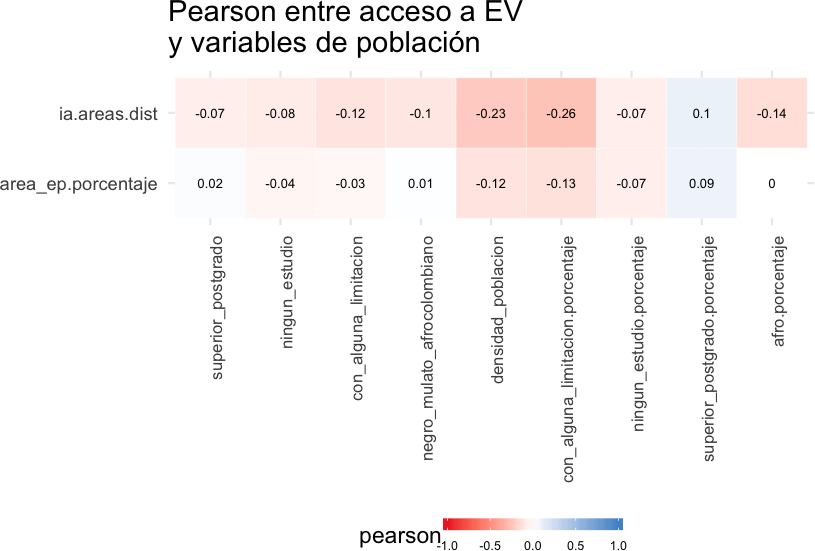
\includegraphics[width=1\linewidth]{tesis-unigis_files/figure-latex/tile-ev-poblacion-pearson-1} 

}

\caption{Coeficiente Pearson entre acceso a EV y variables de población}\label{fig:tile-ev-poblacion-pearson}
\end{figure}

\begin{figure}[H]

{\centering 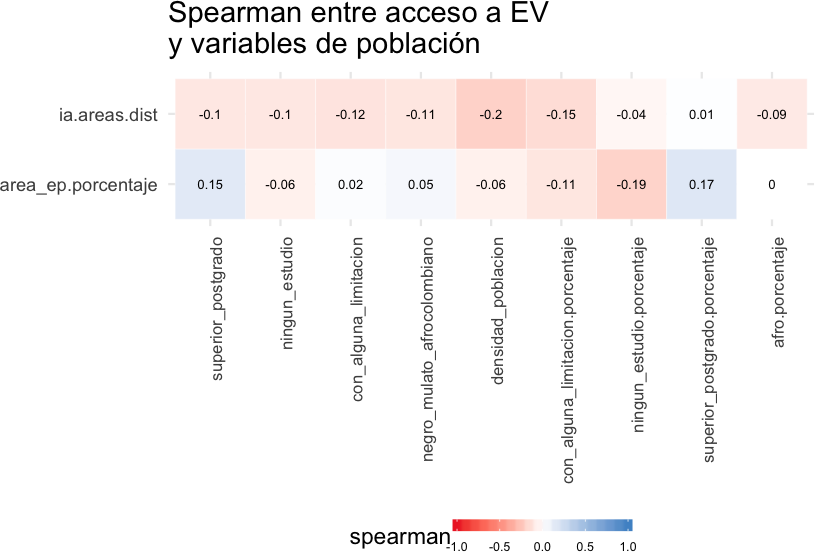
\includegraphics[width=1\linewidth]{tesis-unigis_files/figure-latex/tile-ev-poblacion-spearman-1} 

}

\caption{Coeficiente Spearman entre acceso a EV y variables de población}\label{fig:tile-ev-poblacion-spearman}
\end{figure}

El conjunto de variables sobre el uso de los predios y sus coeficientes
de correlación con las variables dependientes se muestran en las figuras
\ref{fig:tile-ev-uso-pearson} y \ref{fig:tile-ev-uso-spearman}. De nuevo
las correlaciones son bajas, y aparentemente poco explicativas de los
índices de acceso. Las variables de uso de los predios que mejor se
relacionan con los índices son:
\texttt{uso\ de\ unidad\ económica\ {[}\%{]}} y el
\texttt{viviendas\ tipo\ cuarto\ {[}\%{]}}.

\begin{figure}[H]

{\centering 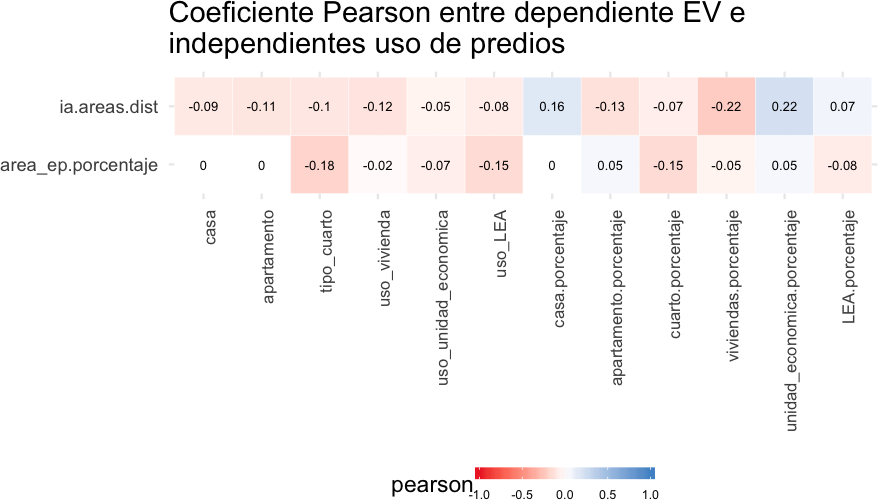
\includegraphics[width=1\linewidth]{tesis-unigis_files/figure-latex/tile-ev-uso-pearson-1} 

}

\caption{Coeficiente Pearson entre acceso a EV y variables de uso de los predios}\label{fig:tile-ev-uso-pearson}
\end{figure}

\begin{figure}[H]

{\centering 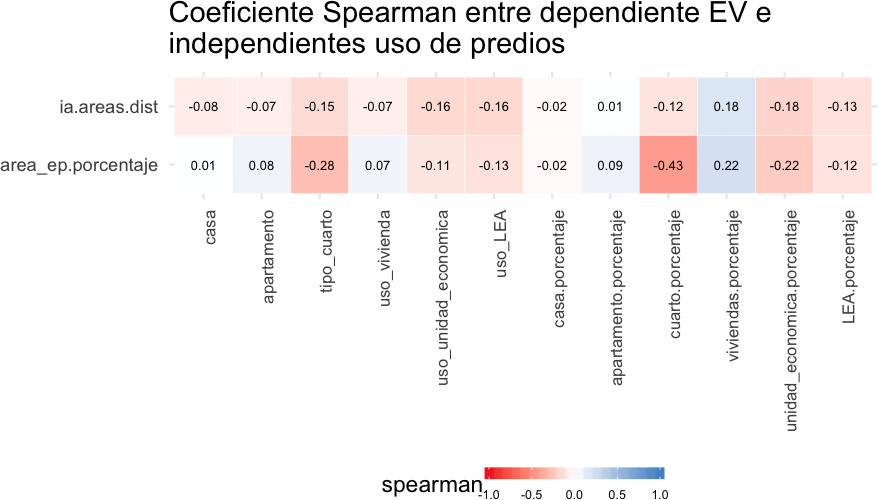
\includegraphics[width=1\linewidth]{tesis-unigis_files/figure-latex/tile-ev-uso-spearman-1} 

}

\caption{Coeficiente Spearman entre acceso a EV y variables de uso de los predios}\label{fig:tile-ev-uso-spearman}
\end{figure}

El último bloque de variables indaga sobre las áreas y proporciones de
las manzanas de cada sector censal y la vocación como pública o privada
de los espacios dentro de un sector urbano. Las figuras
\ref{fig:tile-ev-fisica-pearson} y \ref{fig:tile-ev-fisica-spearman}
muestran que el área media de las manzanas
(\texttt{área\ media\ de\ manzana}) de los sectores urbanos se relaciona
de forma positiva con ambos índices de acceso, mucho más fuertemente que
las variables poblacionales y de uso de predios. Aunque parece haber una
fuerte correlación de los indicadores de acceso con las áreas privadas,
públicas y del sector urbano, estas hacen parte de los cálculos que
generan estos índices, produciendo en efecto ficticio en la correlación,
razón por la que se incluyen en la modelación.

\begin{figure}[H]

{\centering 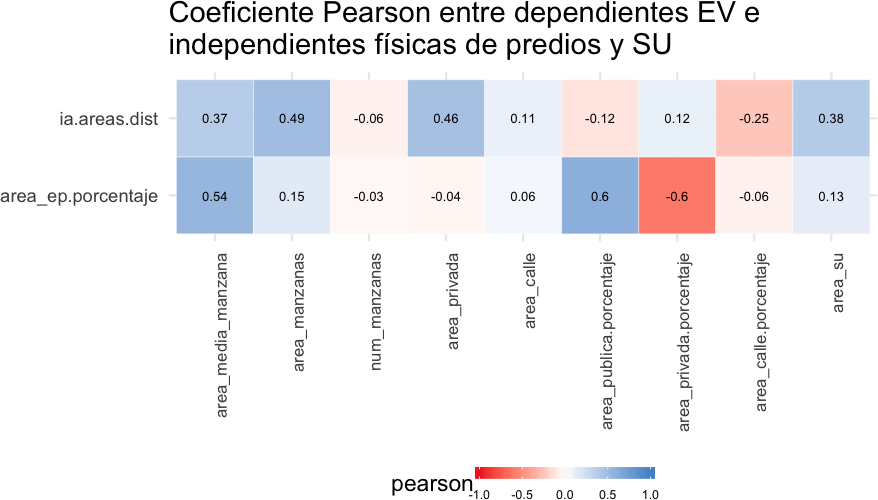
\includegraphics[width=1\linewidth]{tesis-unigis_files/figure-latex/tile-ev-fisica-pearson-1} 

}

\caption{Coeficiente Pearson entre acceso a EV y variables sobre aspectos físicos de las manzanas y SU}\label{fig:tile-ev-fisica-pearson}
\end{figure}

\begin{figure}[H]

{\centering 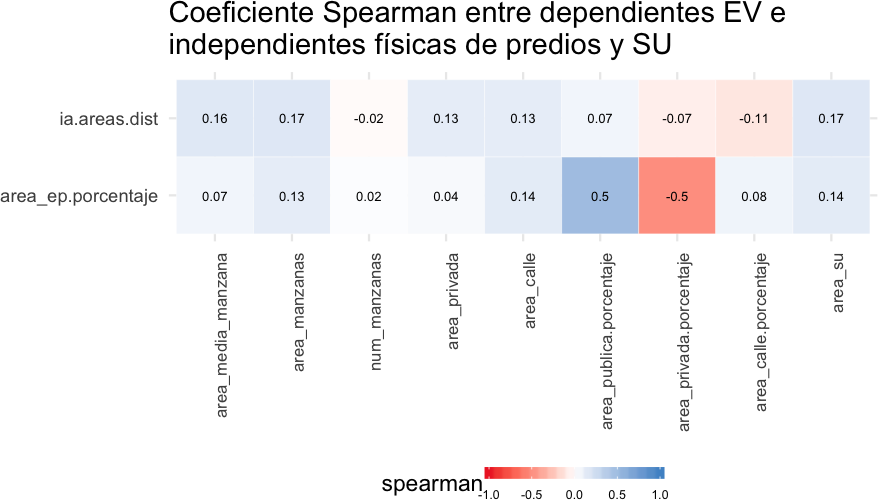
\includegraphics[width=1\linewidth]{tesis-unigis_files/figure-latex/tile-ev-fisica-spearman-1} 

}

\caption{Coeficiente Spearman entre acceso a EV y variables sobre aspectos físicos de las manzanas y SU}\label{fig:tile-ev-fisica-spearman}
\end{figure}

En resumen, las variables independientes escogidas para los modelos
lineales son:

\begin{itemize}
\item
  Para el área de EV {[}\%{]} los predictores seleccionados son
  \texttt{ningun\ estudio\ {[}\%{]}}, \texttt{área\ media\ de\ manzana},
  \texttt{vivienda\ tipo\ cuarto\ {[}\%{]}}.
\item
  Para razón área-distancia los predictores seleccionados son
  \texttt{densidad\ de\ población},
  \texttt{con\ alguna\ limitación\ {[}\%{]}},
  \texttt{uso\ de\ unidad\ económica\ {[}\%{]}},
  \texttt{área\ media\ de\ manzana}.
\end{itemize}

\subsection{Modelos de regresión lineal
EV}\label{modelos-de-regresiuxf3n-lineal-ev}

La tabla \ref{tab:coef-lm-ptjeAEV} muestra los coeficientes de la
regresión para el porcentaje de EV; la tabla \ref{tab:coef-lm-areadist}
muestra los coeficientes de la regresión para índice áreas-distancia, y
la tabla \ref{tab:ajuste-lmev-pob-predios} resume las métricas de ajuste
de ambos modelos.

Los resultados de los test Shapiro-Wilk indican no normalidad en los
residuos en ambos modelos, heterocedasticidad como muestra el test
Breusch-Pagan y posibles no linealidades como se observa en las gráficas
diagnósticas de la regresión de ambos modelos (ver figuras
\ref{fig:diagn-lm-areaptj-sel} y \ref{fig:diagn-lm-areadist-sel}). El
nivel explicativo de la variabilidad de los datos de ambos modelos es
bajo. Sin embargo, el ajuste de ambos modelos tiene media de los
residuos muy cercanas a 0, al igual que el error cuadrático medio (MSE).

Las variables significativas para el área de EV {[}\%{]} son
\texttt{área\ media\ de\ manzana},
\texttt{vivienda\ tipo\ cuarto\ {[}\%{]}}. Estos resultados muestran que
no existe evidencia significativa de que el acceso a EV en un SU esté
relacionado con variables étnicas, de discapacidad o de acceso a la
educación. Sin embargo es muy importante la relación positiva con
aspectos estructurales representados por el área media de las manzanas y
una relación negativa con el porcentaje de viviendas tipo cuarto, estas
últimas concentradas en la zona centro y de ladera del área urbana de
Santiago de Cali (ver figura \ref{fig:mapas-usopredios-cont}).

Para la relación de área distancia se confirma la significancia de
\texttt{área\ media\ de\ manzana} y, en ausencia de la variable
\texttt{vivienda\ tipo\ cuarto\ {[}\%{]}}, se incorpora
\texttt{uso\ de\ unidad\ económica\ {[}\%{]}} que exhibe un patrón
espacial similar. A diferencia del índice local de acceso, en
\texttt{razón\ área-distancia} se evidenció una relación negativa con el
porcentaje de personas con alguna limitación.

Para la siguientes fases se ignoraron las variables no significativas de
los modelos lineales.

\begin{table}[H]

\caption{\label{tab:coef-lm-ptjeAEV}Coeficientes OLS de Porcentaje de EV}
\centering
\begin{tabular}{lrrrr}
\toprule
Término & Estimado & Error std. & t-valor & Pr(>|t|)\\
\midrule
Intercepto & 0.03978 & 0.00826 & 4.81799 & 0.00000\\
ningun estudio [\%] & 0.05796 & 0.03665 & 1.58150 & 0.11474\\
área media de manzana & 0.75792 & 0.06561 & 11.55207 & 0.00000\\
vivienda tipo cuarto [\%] & -0.12801 & 0.04332 & -2.95478 & 0.00336\\
\bottomrule
\end{tabular}
\end{table}

\begin{table}[H]

\caption{\label{tab:coef-lm-areadist}Coeficientes OLS de áreas-distancia}
\centering
\begin{tabular}{lrrrr}
\toprule
Término & Estimado & Error std. & t-valor & Pr(>|t|)\\
\midrule
Intercepto & 0.08879 & 0.02062 & 4.30576 & 0.00002\\
densidad de población & -0.02263 & 0.03137 & -0.72126 & 0.47127\\
con alguna limitación [\%] & -0.10709 & 0.03701 & -2.89321 & 0.00407\\
uso de unidad económica [\%] & 0.08831 & 0.03838 & 2.30125 & 0.02201\\
área media de manzana & 0.46186 & 0.08632 & 5.35076 & 0.00000\\
\bottomrule
\end{tabular}
\end{table}

\begin{table}[H]

\caption{\label{tab:ajuste-lmev-pob-predios}Resumen métricas de ajuste OLS Indice contenedor (EV) y de acceso área-distancia }
\centering
\begin{tabular}{lrr}
\toprule
medidasfit & EV & Área-Distancia\\
\midrule
Shapiro-Wilk & 0.76782 & 0.55302\\
SW p-value & 0.00000 & 0.00000\\
Breusch-Pagan & 12.98572 & 51.60213\\
BP p-value & 0.00151 & 0.00000\\
Media Residuos & 0.00000 & 0.00000\\
\addlinespace
MSE & 0.00607 & 0.00923\\
adj-Rsquare & 0.29656 & 0.17542\\
AIC & -737.84913 & -597.63015\\
Log likelihood & 372.92456 & 303.81507\\
\bottomrule
\end{tabular}
\end{table}

\begin{figure}[H]

{\centering 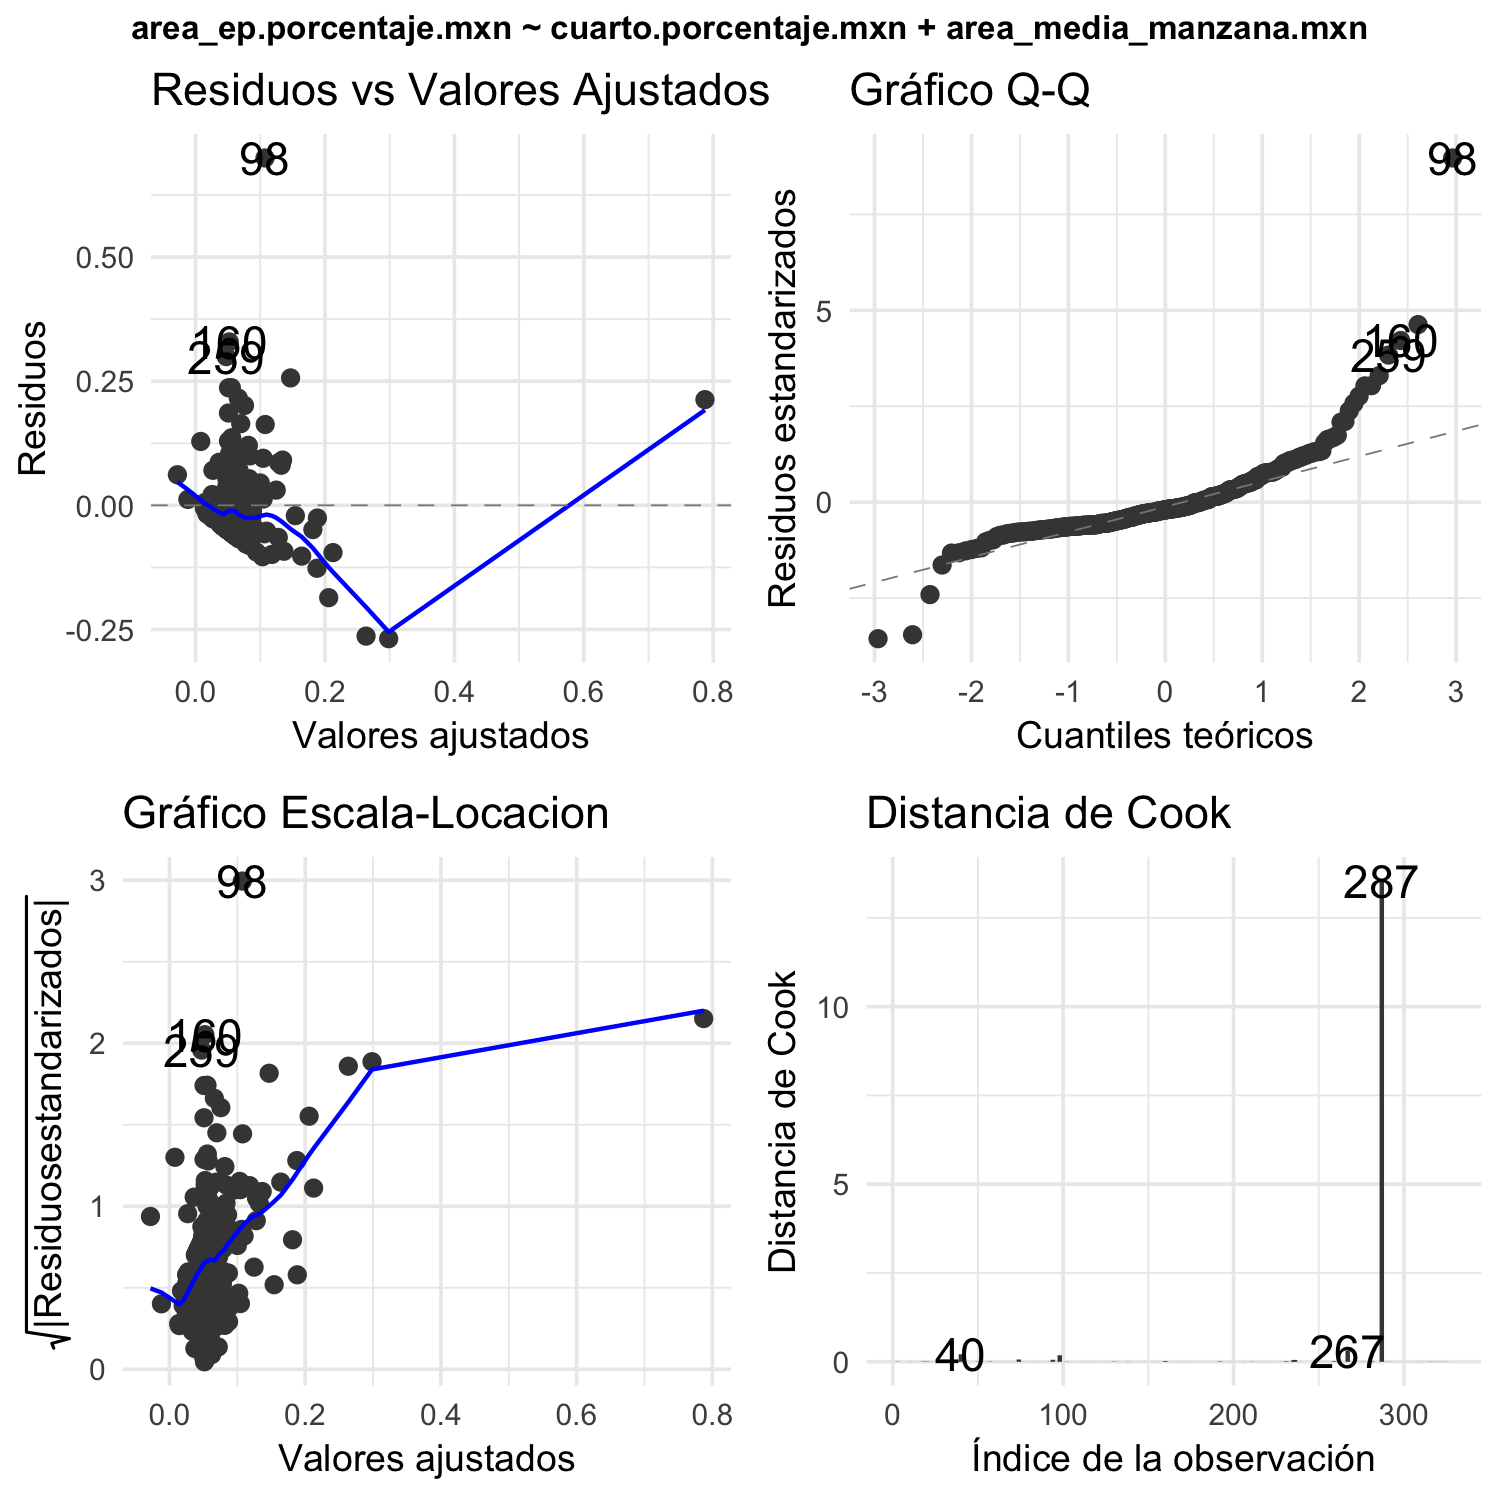
\includegraphics[width=1\linewidth]{tesis-unigis_files/figure-latex/diagn-lm-areaptj-sel-1} 

}

\caption{Gráficas diagnósticas para OLS del porcentaje de EV }\label{fig:diagn-lm-areaptj-sel}
\end{figure}

\begin{figure}[H]

{\centering 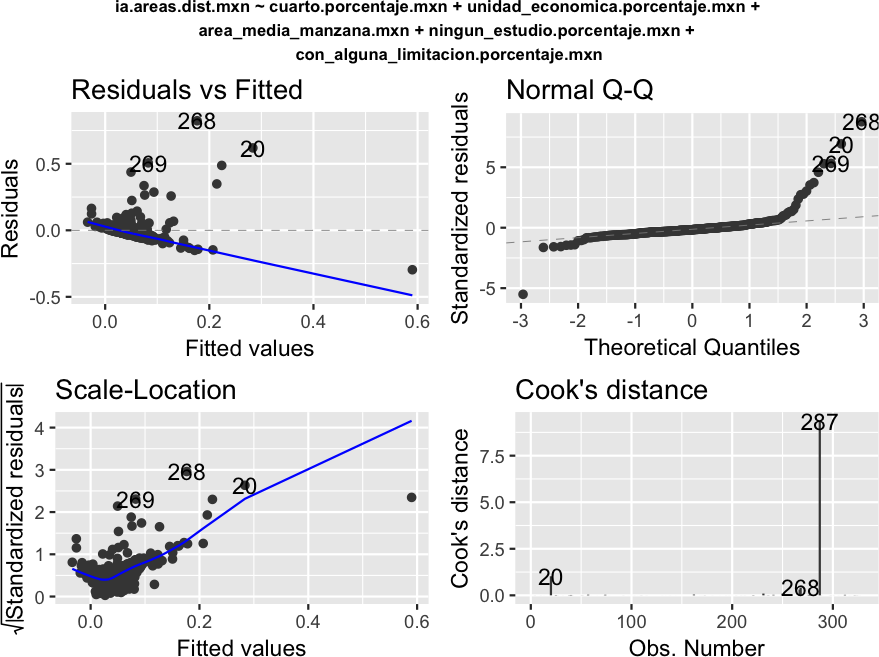
\includegraphics[width=1\linewidth]{tesis-unigis_files/figure-latex/diagn-lm-areadist-sel-1} 

}

\caption{Gráficas diagnósticas para OLS de índice área-distancia}\label{fig:diagn-lm-areadist-sel}
\end{figure}

\subsection{Modelado espacial de espacios
verdes}\label{modelado-espacial-de-espacios-verdes}

El proceso de ajuste de los modelos geoestadísticos para el análisis de
espacios verdes hace uso de los mismos elementos metodológicos usados
para la cobertura de copa. Se usaron las dos matrices de vecindad usando
un kernel de vecindad \emph{Queen} \(W_q\) y otro con base en un radio
de búsqueda de 1 kilómetro \(W_d\) usadas en el análisis del AU (ver
figura \ref{fig:ws-su-reg}).

\subsubsection{Autocorrelación variables
dependientes}\label{autocorrelaciuxf3n-variables-dependientes-1}

Se analizó la autocorrelación de las variables dependientes para
encontrar agrupaciones existentes en los datos que pueden ser explicados
por la estructura de vecindad. Los resultados de los test de Moran'I
para ambas variables dependientes muestran que existen patrones de
agrupamiento y puede rechazarse la hipótesis nula de que los procesos
espaciales subyacentes son aleatorios (ver tablas
\ref{tab:moran-areaep-w} y \ref{tab:moran-areadist-w}).

Ambos diseños de matriz revelan presencia clara de autocorrelación
espacial. La matriz \(W_q\) captura mejor la autocorrelación de ambos
indicadores. El indicador \texttt{razón\ área-distancia} exhibe un valor
de autocorrelación mucho más alto que \texttt{área\ de\ EV\ {[}\%{]}}.
El cálculo del índice \texttt{razón\ área-distancia} en su construcción
usa una distancia de radio de búsqueda de 1 kilómetro. En su definición
el indicador está influenciado por sus vecinos por lo que se forman
grupos o \emph{clusters} alrededor de ciertos sectores urbanos. Resulta
pues interesante no sea \(W_d\) la que capture mejor el agrupamiento.

Los mapas LISA para ambos indicadores de acceso a EV usando la matriz
\(W_q\) muestran los grupos de sectores autocorrelacionados (figuras
\ref{fig:mapas-lisa-areaep-wq} y \ref{fig:mapas-lisa-areadist-wq}). Los
grupos formados muestran agrupaciones de alto acceso a EV en relación al
resto de la ciudad. Se aprecia que se forman \emph{clusters} alrededor
de cuatro zonas en el caso del porcentaje de área de EV y dos para el
indicador de relación áreas-distancia, coincidentes con el anterior.
Esos sectores albergan equipamientos de ciudad como un cementerio de
gran tamaño, las universidades y zonas conservadas de riberas de ríos.
El grupo que se forma al oriente de la ciudad es donde se encuentra la
laguna del Pondaje.

\begin{table}[H]

\caption{\label{tab:moran-areaep-w}Test de Moran - Porcenatje de EV para $W_q$ y $W_d$}
\centering
\begin{tabular}{lrr}
\toprule
  & $W_q$ & $W_d$\\
\midrule
Estadístico Moran I & 0.10462 & 0.05377\\
Expectativa & -0.00305 & -0.00308\\
Varianza & 0.00101 & 0.00076\\
Desviación estándar de Moran I & 3.39376 & 2.06018\\
p-valor & 0.00034 & 0.01969\\
\bottomrule
\end{tabular}
\end{table}

\begin{table}[H]

\caption{\label{tab:moran-areadist-w}Test de Moran - Razón área distancia para $W_{q}$ y $W_{d}$}
\centering
\begin{tabular}{lrr}
\toprule
  & $W_{q}$ & $W_{d}$\\
\midrule
Estadístico Moran I & 0.78314 & 0.67779\\
Expectativa & -0.00305 & -0.00308\\
Varianza & 0.00102 & 0.00077\\
Desviación estándar de Moran I & 24.62379 & 24.51886\\
p-valor & 0.00000 & 0.00000\\
\bottomrule
\end{tabular}
\end{table}

\begin{figure}[H]

{\centering 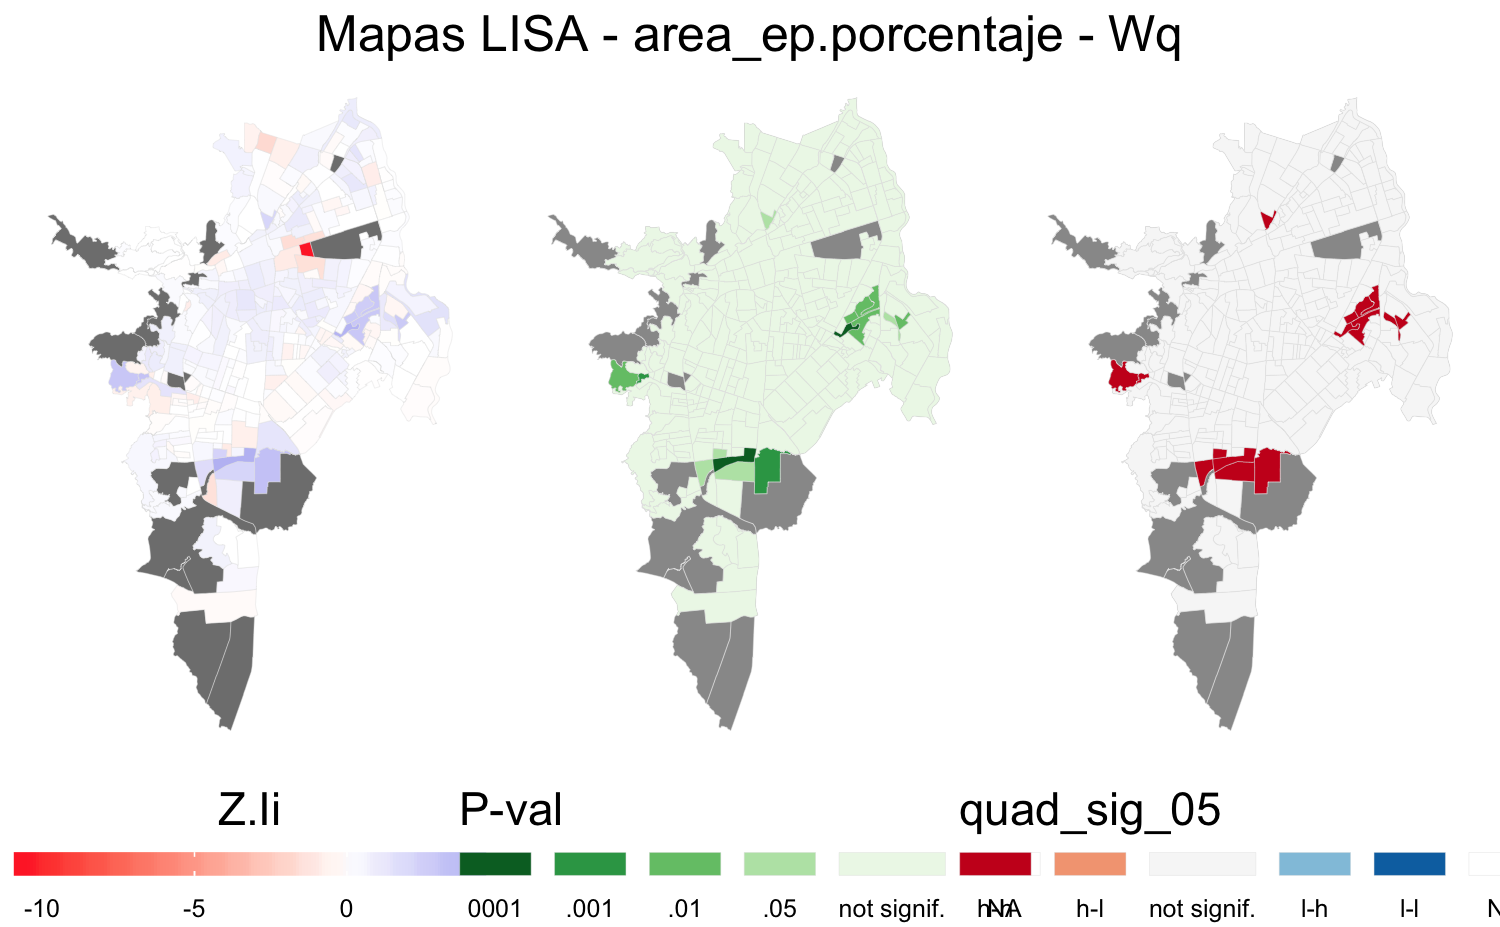
\includegraphics[width=1\linewidth]{tesis-unigis_files/figure-latex/mapas-lisa-areaep-wq-1} 

}

\caption{Mapas LISA para la matriz $W_q$ de área de EV [\%]}\label{fig:mapas-lisa-areaep-wq}
\end{figure}

\begin{figure}[H]

{\centering 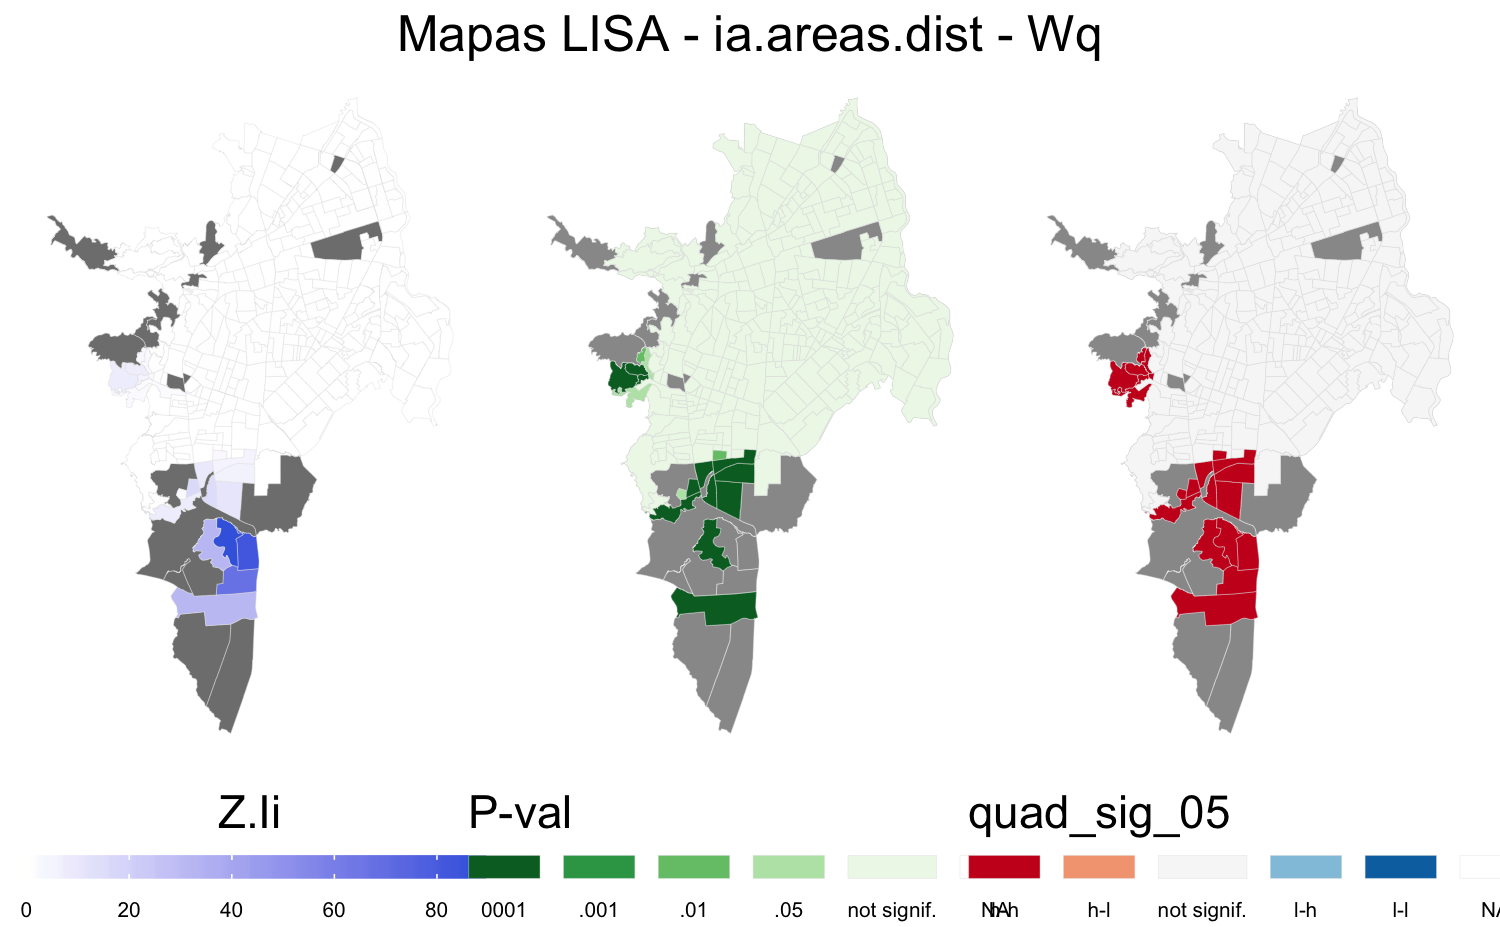
\includegraphics[width=1\linewidth]{tesis-unigis_files/figure-latex/mapas-lisa-areadist-wq-1} 

}

\caption{Mapas LISA para la matriz $W_q$ de razón área-distancia}\label{fig:mapas-lisa-areadist-wq}
\end{figure}

\subsubsection{Autocorrelación residuos de los
OLS}\label{autocorrelaciuxf3n-residuos-de-los-ols-1}

Para evaluar la utilidad de aplicar modelos espaciales de regresión se
examinó la existencia de autocorrelación en los residuos de los modelos
de regresión lineal. Se comparó si alguno de las estructuras de vecindad
produce resultados significativamente mejores en la detección de
autocorrelación espacial.

La tabla \ref{tab:moran-resareaep-w} muestra que ambos diseños de matriz
\(W\) presentan un valor de Moran Global mayor que 0 y significativo
para los residuos del OLS del porcentaje de área de EV, al igual que
para los residuos del OLS del indicador áreas-distancia (ver tabla
\ref{tab:moran-resareadist-w}).

En ambos modelos el resultado de autocorrelación espacial sugiere que,
al introducir retardos espaciales y la estructura de vecindad, pueden
mejorar la estimación de los coeficientes de la regresión y las métricas
de desempeño del ajuste.

\begin{table}[H]

\caption{\label{tab:moran-resareaep-w}Test de Moran - Residuos de OLS Porcentaje EV $W_q$ y $W_d$}
\centering
\begin{tabular}{lrr}
\toprule
  & $W_q$ & $W_d$\\
\midrule
Estadístico Moran I & 0.11636 & 0.04201\\
Expectativa & -0.00305 & -0.00308\\
Varianza & 0.00108 & 0.00082\\
Desviación estándar de Moran I & 3.63225 & 1.57642\\
p-valor & 0.00014 & 0.05746\\
\bottomrule
\end{tabular}
\end{table}

\begin{table}[H]

\caption{\label{tab:moran-resareadist-w}Test de Moran - Residuos de OLS relación áreas distancias para $W_q$ y $W_d$}
\centering
\begin{tabular}{lrr}
\toprule
  & $W_q$ & $W_d$\\
\midrule
Estadístico Moran I & 0.61445 & 0.58256\\
Expectativa & -0.00305 & -0.00308\\
Varianza & 0.00105 & 0.00080\\
Desviación estándar de Moran I & 19.04546 & 20.76452\\
p-valor & 0.00000 & 0.00000\\
\bottomrule
\end{tabular}
\end{table}

\subsubsection{Modelo espacial porcentaje de espacio
verde}\label{modelo-espacial-porcentaje-de-espacio-verde}

Dado que la matriz \(W_q\) capturó mejor la asociación espacial en los
datos para ambos indicadores de acceso a EV, se realizó el ajuste de los
modelos espaciales solo con ese diseño.

Las métricas de ajuste de los modelos de porcentaje de área de EV (ver
tabla \ref{tab:tabla-comp-modelos-areaep}) muestran que los modelos
espaciales logran eliminar la autocorrelación espacial global en los
residuos. Todos los modelos mejoran las métricas de error respecto del
OLS y ninguno logra la normalidad ni la homocedasticidad en los
residuos.

Al comparar los resultados usando el desempeño en AIC se identificó al
modelo SEM con el mejor ajuste. El modelo SEM logra eliminar la
autocorrelación espacial global en los residuos. El coeficiente
\(\lambda\) del término autorregresivos es alto y significativo (tabla
\ref{tab:cauto-sem-areaep}), lo que sugiere que no es necesario plantear
efectos de la variables dependientes rezagadas, y que es posible que ese
efecto sea por otras variables no tenidas en cuenta. Esta lectura del
SEM es interesante y consistente con el significado local del indicador
porcentaje de área de EV.

El resultado del modelo SEM confirma la significancia y efecto positivo
para el acceso EV del área de promedio de la manzana en un SU. La
presencia de viviendas tipo cuarto, con coeficiente negativos, es un
factor que coincide con la disminución de área de EV disponible (ver
tabla \ref{tab:coef-sem-areaep}). Existen cambios y ajustes en los
valores de los coeficientes con relación al modelo OLS, que dadas las
mejoras en las métricas de ajuste hacen más confiables las estimaciones.

\begin{table}[H]

\caption{\label{tab:tabla-comp-modelos-areaep}Metricas de ajuste para los modelos de porcentaje de área de EV con $W_q$}
\centering
\begin{tabular}{lrrrr}
\toprule
medidasfit & OLS & SAR & SEM & SD\\
\midrule
Globla Moran'I & 0.11636 & 0.04015 & -0.00817 & -0.00602\\
GMI p-value & 0.00014 & 0.09378 & 0.56220 & 0.53618\\
Shapiro-Wilk & 0.76782 & 0.76040 & 0.75813 & 0.76159\\
SW p-value & 0.00000 & 0.00000 & 0.00000 & 0.00000\\
Breusch-Pagan & 12.98572 & 13.97239 & 11.07822 & 13.54161\\
\addlinespace
BP p-value & 0.00151 & 0.00092 & 0.00393 & 0.00891\\
Media Residuos & 0.00000 & 0.00000 & 0.00000 & 0.00000\\
MSE & 0.00607 & 0.00596 & 0.00581 & 0.00576\\
adj-Rsquare & 0.29656 & NA & NA & NA\\
Nagelkerke pseudo-R-squared & NA & 0.31043 & 0.32222 & 0.32798\\
\addlinespace
AIC & -737.84913 & -740.39306 & -746.06370 & -744.87233\\
Log likelihood & 372.92456 & 375.19653 & 378.03185 & 379.43617\\
\bottomrule
\end{tabular}
\end{table}

\begin{table}[H]

\caption{\label{tab:coef-sem-areaep}Coeficientes del modelo SEM de porcentaje de área de EV}
\centering
\begin{tabular}{lrrrr}
\toprule
Término & Estimado & Error std. & t-valor & Pr(>|t|)\\
\midrule
Intercepto & 0.049 & 0.007 & 7.116 & 0.000\\
vivienda tipo cuarto [\%] & -0.098 & 0.042 & -2.355 & 0.019\\
área media de manzana & 0.771 & 0.065 & 11.803 & 0.000\\
\bottomrule
\end{tabular}
\end{table}

\begin{table}[H]

\caption{\label{tab:cauto-sem-areaep}Coeficiente de autocorrelación modelo SEM de porcentaje de área de EV}
\centering
\begin{tabular}{lll}
\toprule
$\lambda$ & Likelihood ratio & p-valor\\
0.259 & 10.215 & 0.001\\
\bottomrule
\end{tabular}
\end{table}

\subsubsection{Modelo espacial del índice de acceso
área-distancia}\label{modelo-espacial-del-uxedndice-de-acceso-uxe1rea-distancia}

Las métricas de ajuste de los modelos de indicador área-distancia (ver
tabla \ref{tab:tabla-comp-modelos-areasdist}) muestran que los modelos
espaciales logran eliminar la autocorrelación espacial global en los
residuos. Todos los modelos mejoran las métricas de error respecto del
OLS, en particular el \emph{Nagelkerke}, equivalente al
\emph{adj-Rsquare}, que mide el nivel explicativo del modelo en la
variabilidad de los datos, subiendo de \(\simeq 0.17\) a
\(\simeq 0.74\).

Al comparar los resultados usando el desempeño en AIC se identificó al
modelo SD con el mejor ajuste. El modelo SD logra eliminar la
autocorrelación espacial global en los residuos. El coeficiente \(\rho\)
del término autorregresivos es muy alto y significativo (tabla
\ref{tab:cauto-sd-areasdist}), lo que sugiere que los efectos de las
variables dependientes rezagadas so significativos. Existen cambios y
ajustes en los valores de los coeficientes con relación al modelo OLS,
que dadas las mejoras en las métricas de ajuste hacen más confiables las
estimaciones (y se corrobora con las gráficas diagnósticas de la figura
\ref{fig:diag-model-areasdist-espaciales}).

El resultado del modelo SD confirmó la significancia y efecto positivo
pero bajo en el acceso a EV de contar con unidades económicas dentro del
SU. Es significativo y fuerte en el acceso a EV estar al rededor de SUs
con manzanas de área promedio grande. Por otro lado se desestima que
exista una relación con la variable porcentaje personas con alguna
limitación (ver tabla \ref{tab:coef-sd-areasdist}). La escogencia del
modelo SD se ajusta consistentemente con el propósito del indicador
áreas-distancia de medir el acceso en un SU más allá de su límite
geográfico.

\begin{table}[H]

\caption{\label{tab:tabla-comp-modelos-areasdist}Metricas de ajuste para los modelos de áreas-distancia de EV}
\centering
\begin{tabular}{lrrrr}
\toprule
medidasfit & OLS & SAR & SEM & SD\\
\midrule
Globla Moran'I & 0.61445 & -0.17676 & -0.17439 & -0.13656\\
GMI p-value & 0.00000 & 1.00000 & 1.00000 & 0.99998\\
Shapiro-Wilk & 0.55302 & 0.50369 & 0.49323 & 0.59974\\
SW p-value & 0.00000 & 0.00000 & 0.00000 & 0.00000\\
Breusch-Pagan & 51.60213 & 15.79282 & 5.19151 & 73.10115\\
\addlinespace
BP p-value & 0.00000 & 0.00125 & 0.15830 & 0.00000\\
Media Residuos & 0.00000 & 0.00000 & 0.00000 & 0.00000\\
MSE & 0.00923 & 0.00279 & 0.00275 & 0.00252\\
adj-Rsquare & 0.17542 & NA & NA & NA\\
Nagelkerke pseudo-R-squared & NA & 0.70286 & 0.70042 & 0.74346\\
\addlinespace
AIC & -597.63015 & -928.40318 & -925.72082 & -970.74368\\
Log likelihood & 303.81507 & 470.20159 & 468.86041 & 494.37184\\
\bottomrule
\end{tabular}
\end{table}

\begin{table}[H]

\caption{\label{tab:coef-sd-areasdist}Coeficientes del modelo SD índice de relación área distancia de EV}
\centering
\begin{tabular}{lrrrr}
\toprule
Término & Estimado & Error std. & t-valor & Pr(>|t|)\\
\midrule
Intercepto & -0.027 & 0.017 & -1.626 & 0.104\\
uso de unidad económica [\%] & 0.067 & 0.028 & 2.429 & 0.015\\
área media de manzana & 0.015 & 0.048 & 0.314 & 0.754\\
con alguna limitación [\%] & -0.030 & 0.022 & -1.333 & 0.183\\
uso de unidad económica [\%] (retardada) & -0.038 & 0.037 & -1.036 & 0.300\\
\addlinespace
área media de manzana (retardada) & 0.694 & 0.101 & 6.870 & 0.000\\
con alguna limitación [\%] (retardada) & 0.063 & 0.035 & 1.786 & 0.074\\
\bottomrule
\end{tabular}
\end{table}

\begin{table}[H]

\caption{\label{tab:cauto-sd-areasdist}Coeficiente de autocorrelación modelo SD índice de relación área distancia de EV}
\centering
\begin{tabular}{lll}
\toprule
$\rho$ & Likelihood ratio & p-valor\\
0.747 & 255.817 & 0\\
\bottomrule
\end{tabular}
\end{table}

\begin{figure}[H]

{\centering 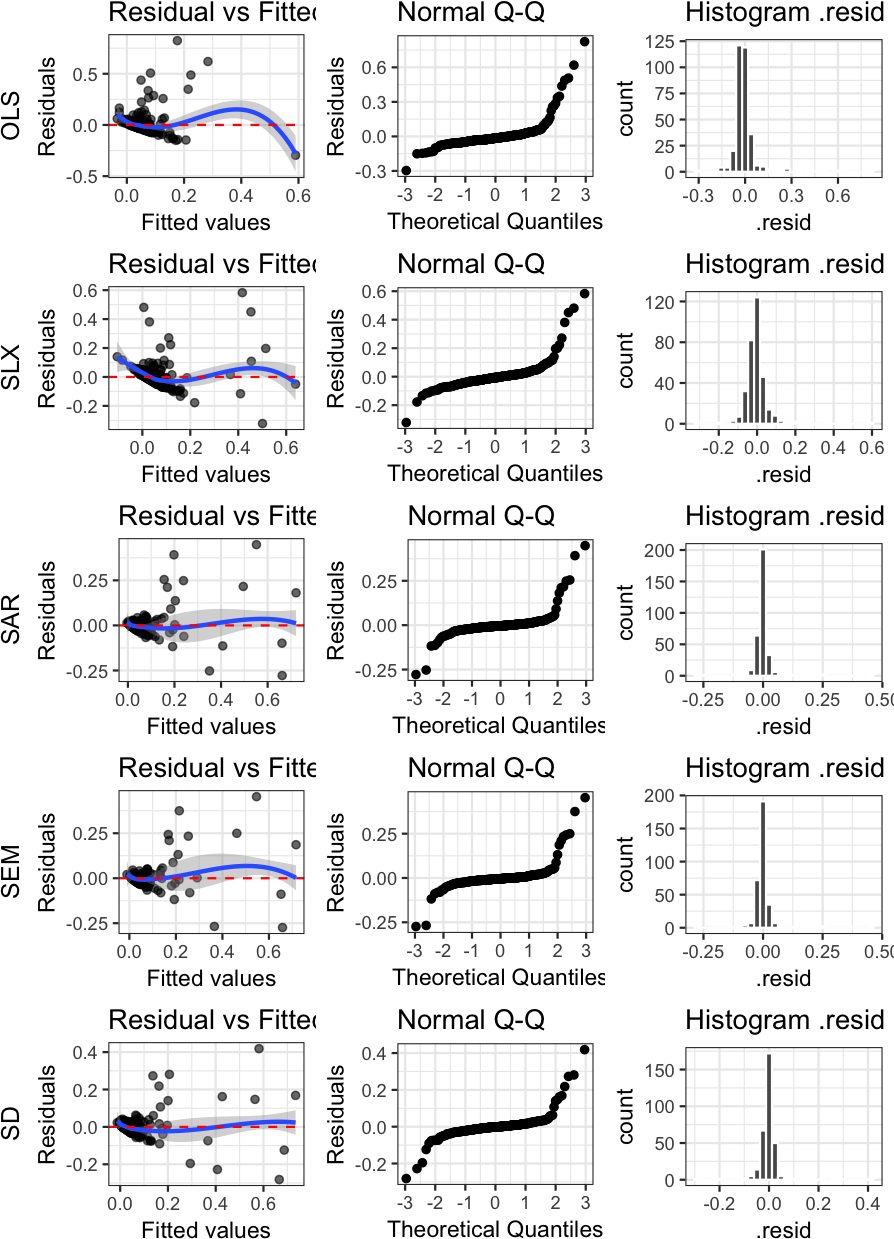
\includegraphics[width=1\linewidth]{tesis-unigis_files/figure-latex/diag-model-areasdist-espaciales-1} 

}

\caption{Diagnóstico comparativo entre modelos espaciales del indicador área-distancia}\label{fig:diag-model-areasdist-espaciales}
\end{figure}

\chapter{Discusión}\label{discusion}

Los modelos realizados son un intento por capturar evidencia empírica
sobre el nivel explicativo de un conjunto de condiciones de la población
y las condiciones de vida que provee la ciudad de Cali en lo que a
beneficios ambientales se refiere. El modelo no es la realidad ni prueba
de causalidad, es un instrumento para cuantificar la relación entre
algunas de esas dimensiones teniendo certeza de su potencial asociación.
El uso de modelos espaciales indaga sobre los patrones espaciales de
esas variables, lo que permite la identificación de zonas que agrupan
características altas de esos servicios con los patrones espaciales de
las condiciones de la población y de la estructura urbana. Los análisis
no buscan hacer inferencia sobre la población, pues no son una muestra,
son la población completa de arboles, espacio verde y los datos del
censo. En este sentido los coeficientes y su representatividad son sobre
la población, y se interpretan como la importancia relativa de esas
variables sobre las otras.

Entre las posibilidades que ofrece el código como herramienta
cartográfica está la de producir y reproducir múltiples mapas, en lugar
de uno solo con mucho detalle como respuestas a las limitaciones
tecnológicas y de costos de la cartografía impresa, lo que redunda en
mejor información para los análisis. Debido a las restricciones de
longitud en la presentación de este texto académico no fueron incluidos
la totalidad de gráficos realizados que se pueden reproducir con los
\emph{scripts} del repositorio del trabajo. Los métodos gráficos como
los mapas de LISA permiten ampliar la interpretación de los mecanismos
de ajuste de los modelos espaciales y de la combinación lineal de los
términos. Estos mapas junto con los mapas temáticos de cada una de las
variables, los gráficos de dispersión de las distribuciones
multivariadas son una estrategia eficaz para lidiar con las dificultades
para analizar conjuntos de datos multidimensionales y espaciales. Los
métodos de ajuste espacial y la comparación entre distintos modelos
permitieron obtener resultados confiables de la estimación de
coeficientes.

Hay que resaltar el uso de herramientas libres como \textbf{R} (R Core
Team, \protect\hyperlink{ref-R-base}{2017}), \textbf{Rstudio} y los
diferentes paquetes del ecosistema del CRAN (Hornik,
\protect\hyperlink{ref-R-cran}{2018}), que favorecen la
reproductibilidad y diseminación del conocimiento científico. El
esfuerzo y la curva de aprendizaje de herramientas como
\textbf{Bookdown} (Xie, \protect\hyperlink{ref-R-bookdown}{2018}) y
\textbf{knitr} (Xie, \protect\hyperlink{ref-R-knitr}{2019}) para la
generación de los contenidos y textos en diferentes formatos, la
reproductibilidad del uso de \emph{scripts} y la posibilidad de publicar
un repositorio del resultado, del proceso y de los datos, no solo vale
la pena como base para la construcción de flujos de trabajo eficientes
en el manejo y divulgación de datos e información ---geográfica---, sino
que son un compromiso ineludible con la construcción de conocimiento
científico y la ética investigativa.

\section{Sobre el arbolado urbano}\label{sobre-el-arbolado-urbano}

En esta investigación se pregunta si el acceso a servicios del AU es una
característica local de los sectores geográficos o si se extienden esos
beneficios a agrupaciones de sectores urbanos vecinos. Al revisar la
literatura es notorio que los indicadores referenciados son expresados
como densidades por unidad de área (ver tabla \ref{tab:ind-AU}). Al usar
el área de los SU (ya sea el área total o la pública) y al delimitar el
conteo de individuos arbóreos o la suma total del área de copa con los
polígonos de cada SU en los indicadores, se está privilegiando una
perspectiva local del acceso a los beneficios del AU. La definición
matemática de los indicadores seleccionados en este trabajo no se aleja
de esta visión local del disfrute, pero promueve matices en la lectura
comparativa entre sectores (porcentaje de cobertura de copa respecto del
área pública del SU) y su importancia a nivel urbano (área total de
copa). El área de copa y el porcentaje de cobertura de copa configuran
dos medidas complementarias sobre un fenómeno local a los SUs, sin
desconocer que en el contexto global del área urbana existen beneficios
ecológicos para toda la ciudad.

Es relevante sobre los resultados de los análisis con diferentes diseños
de matriz, que la vecindad de los SU exhibe un grado de autocorrelación
espacial y por lo tanto los grupos de alta y baja prestación en los
servicios ecosistémicos del AU configuran evidencia de los sesgos
espaciales en la distribución de dichos beneficios, rechazando la
hipótesis nula de distribución espacial aleatoria o uniforme. A pesar de
la persistencia de problemas en la estimación como la no normalidad de
los residuos y la heterocedasticidad ---debidos a posibles no
linealidades entre los predictores y la cobertura de copa--- las
estimaciones mejoran con los modelos con estructura espacial. Aunque las
matrices de vecindad construidas son muy similares entre sí, muestran
que la inclusión \emph{a priori} de una estructura espacial es un
mecanismo eficaz para identificar grupos y probar aspectos teóricos de
la estructura de la autocorrelación. Como trabajo a futuro es necesario
profundizar e incluir criterios teóricos o conocimientos del desarrollo
histórico de la ciudad en la especificación de los modelos y en la
estructura de vecindad.

Al comparar los modelos espaciales seleccionados, se sabe que el SEM
incorpora el componente espacial como información no modelada por los
predictores, y el SD como una influencia de los retardos espaciales de
las variables independientes. Para el área de copa, cuando se acoje la
perspectiva de los retardos (modelo SD con \(W_q\)), solo se considera
significativo el retardo de la variable de porcentaje de viviendas tipo
cuarto, y descarta la variable no retardada. Es decir que la prevalencia
de este tipo de viviendas en un sector urbano está asociado a baja
disponibilidad de copa en sectores vecinos. Cuando se compara esta
interpretación con el modelo SEM con \(W_d\), en contraste, la variable
no retardada de porcentaje de viviendas tipo cuarto resulta
significativa. Es interesante que las diferencias entre las matrices
privilegien la escogencia de un modelo u otro, lo que alerta sobre la
importancia de los supuestos en la escogencia de su estructura ante la
discrepancia entre los resultados, señalando posibles mejoras en la
metodología utilizada.

Sobre los problemas de la estimación, es probable que provengan de
dimensiones no incluidas en el modelo como sugiere el rendimiento del
modelo SEM con la matriz \(W_d\) para el área de copa. En este sentido,
la cercanía a ríos y arterias viales de un mayor desarrollo urbanístico
como el eje longitudinal (figura \ref{fig:mapas-lisa-copaap-wq}), donde
se encuentran la Calle 5 una de las vía más emblemáticas de la ciudad,
puede explicar el agrupamiento de sectores censales con buena cobertura
de AU.

En el caso de la variable de porcentaje de área de copa, los estudios
superiores en la población reflejan el patrón de agrupamiento espacial
de la cobertura de copa pero es poco significativa como variable
retardada, cuestión que pone dudas sobre si el SD proponga una
interpretación acertada o diferente de un modelo autorregresivo puro
como el SAR. De nuevo, estas diferencias indican caminos de mejora
metodológica en lo que se refiere a la selección de modelos y
refinamiento de la formulación de las hipótesis en trabajos futuros.

Estos resultados no son evidencia concluyente para responder si hay un
tipo de modelo más apropiado que otro para capturar la dependencia
espacial en los datos, cuando esta existe. Sin embargo, la lectura
contrastada de los modelos de mayor rendimiento y los diferentes diseños
de la matriz de vecindad convergen en señalar sesgos espaciales,
relacionados con variables de estatus social, la densidad poblacional,
la disponibilidad de zonas verdes y la vocación habitacional o comercial
de un sector urbano.

En ambos modelos la variable más significativa y de mayor valor en el
coeficiente es \textbf{estudios superiores}. Cuando se formulan los
modelos se excluye el uso de variables como porcentaje de población afro
o personas sin estudios por tener una alta correlación negativa con
personas con \textbf{estudios superiores o postgrado} o con su versión
porcentual. Esto implica que los beneficios ambientales son mejores en
sectores con población mejor educada, presumiblemente de mejores
ingresos, (figura \ref{fig:lisa-superiores}), o con preferencia a
habitar espacios con buena arborización y con mayor desarrollo del
espacio público. Estas zonas se caracterizan por la disponibilidad de
espacios verdes y baja densidad de población como indica la
significancia de los coeficientes de estas variables (ver tabla
\ref{tab:coef-sem-copa-wd}). En particular, sobre la disponibilidad de
EV, no es probable que tengan un efecto de difusión o derrame, pues la
creación de estas zonas verdes es algo que ocurre en el proceso de
urbanización del sector y poco o nada cambia después de su creación.

Al indagar sobre cuáles son las zonas que muestran mayores correlaciones
negativas entre las variables sociales y la cobertura de copa, los
resultados muestran un alto grado de segregación de los grupos de
sectores con mayor arborización (figura \ref{fig:lisa-superiores}) y la
población afro (figura \ref{fig:lisa-afro}) y sin estudios, ambos
altamente correlacionadas, como se aprecia en los mapas de LISA y las
matrices de correlación de las figuras \ref{fig:tile-poblacion-pearson}
y \ref{fig:tile-poblacion-spearman}. Existe pues una asociación negativa
entre acceso a educación superior en zonas con prevalencia de población
afro y población sin estudios, que además de la alta segregación laboral
y geográfica que exhiben (Arroyo Mina et~al.,
\protect\hyperlink{ref-arroyo_mina_afrocolombianos_2016}{2016}; Cerón y
Escobar, \protect\hyperlink{ref-ceron_indice_2014}{2014}; Mora y Arcila,
\protect\hyperlink{ref-mora_brechas_2014}{2014}; Pacheco,
\protect\hyperlink{ref-PACHECO2013121}{2013}), está menos beneficiada de
los servicios ambientales provistos por el AU. Estos hallazgos coinciden
con trabajos sobre ciudades en Estados Unidos como en Schwarz et~al.
(\protect\hyperlink{ref-schwarz_trees_2015}{2015}) donde se prueba que
la distribución espacial de árboles está sesgada por la distribución del
ingreso, que a su vez también está relacionada con patrones de
segregación racial.

Este tipo de desigualdades son una responsabilidad de los urbanizadores
y de los gobiernos locales. Es de su interés y responsabilidad dialogar
para construir y propiciar espacios para la siembra y desarrollo de los
individuos arbóreos, pues es fundamental su agencia para reducir brechas
sociales, crear una ciudad con espacio e infraestructura natural que
sostenga los ecosistemas de los que depende la ciudad y la calidad de
vida de sus ciudadanos. Ciudadanos para quienes lo ambiental viene
cobrando más importancia como valor social, y que además se convierte en
una estrategia para mitigar los cambios que pueda traer consigo el
calentamiento global.

\begin{figure}[H]

{\centering 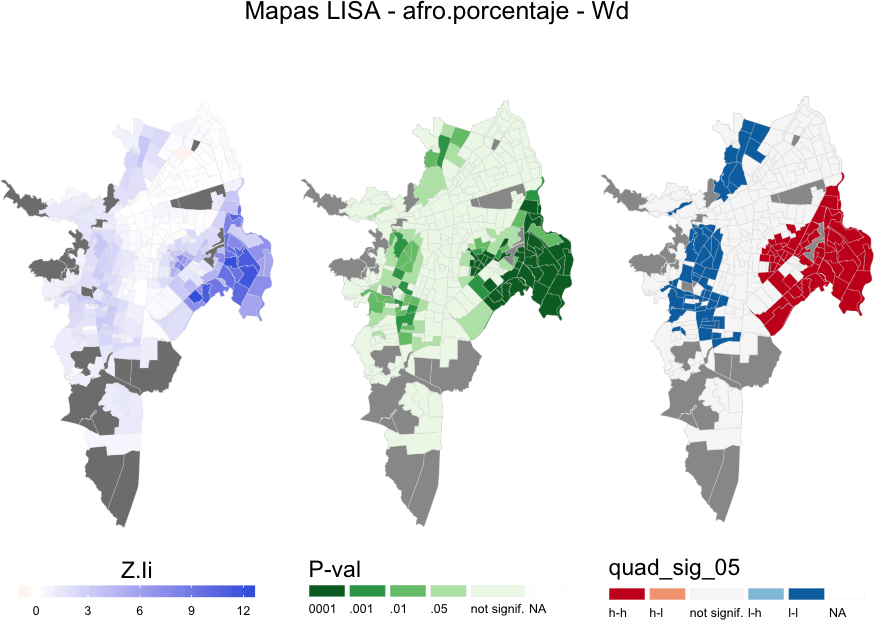
\includegraphics[width=1\linewidth]{tesis-unigis_files/figure-latex/lisa-afro-1} 

}

\caption{Mapas LISA - Porcentaje población afrocolombiana}\label{fig:lisa-afro}
\end{figure}

\begin{figure}[H]

{\centering 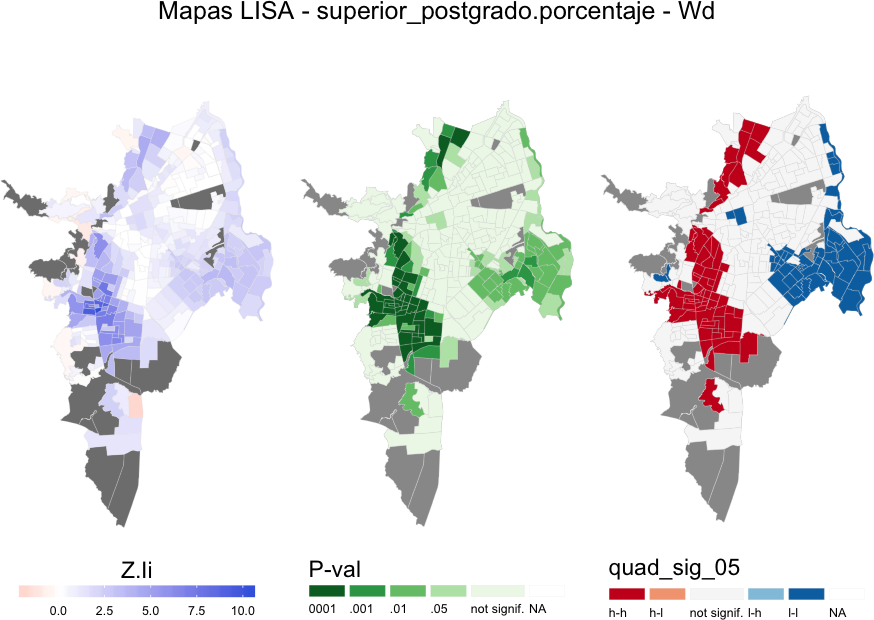
\includegraphics[width=1\linewidth]{tesis-unigis_files/figure-latex/lisa-superiores-1} 

}

\caption{Mapas LISA - Porcentaje población con estudios superiores}\label{fig:lisa-superiores}
\end{figure}

\section{Sobre los espacios verdes}\label{sobre-los-espacios-verdes}

Análogamente al ejercicio realizado con el AU, este trabajo se pregunta
si el acceso a servicios de los EVs es una característica local de los
sectores geográficos o si se extienden esos beneficios a agrupaciones de
sectores urbanos vecinos. En contraste con los indicadores de acceso a
beneficios del AU, en los indicadodres de acceso a EV se diferencia
claramente un enfoque local de uno global (ver tabla \ref{tab:ind-EV}).
Desde la concepción local se define el acceso a EVs en un SU como la
existencia de EVs exclusivamente dentro de ese SU. En el enfoque global
se propone indicadores en los que el acceso está compuesto por aportes
ponderados por la distancia de los EVs al SU, incluyendo aquellos
situados por fuera del SU, ya sea en todo el área de estudio o en un
rango de búsqueda predeterminado. Son dos apuestas conceptuales
distintas para aproximarse al concepto de acceso. Esta investigación usó
un indicador de cada tipo: un indicador local, porcentaje de área de EV
respecto del área del SU y uno global, que define el acceso como la
relación entre el área disponible y el costo de traslado hasta un EV sin
importar si los EVs están estrictamente dentro del SU. En síntesis, el
concepto de acceso admite ambos enfoques, y pueden en trabajos futuros
combinarse en un índice de acceso compuesto.

Al evaluar la autocorrelación espacial de los indicadores propuestos,
ambos presentan un valor significativo y positivo en el Moran'I. Sin
embargo, el indicador de relación área-distancia, en consecuencia con la
concepción global de acceso, obtuvo valores de Moran'I muy superiores al
indicador de porcentaje de EV (ver tablas \ref{tab:moran-resareaep-w} y
\ref{tab:moran-resareadist-w}).

Es relevante en los resultados de los análisis que los grupos de alta
prestación en los servicios ecosistémicos de los EV configuran evidencia
de los sesgos espaciales en la distribución de dichos beneficios. Puede
decirse que la mayor parte de la ciudad tiene bajos valores en el acceso
a EVs y que la población con mejores beneficios está concetrada en el
sur de la ciudad. Como se muestra en los histogramas de distribución de
los valores de ambos indicadores (ver figuras \ref{fig:hist-areaep} y
\ref{fig:hist-areasdist}), la tendencia es a una baja disponibilidad y
acceso a los EV. Puede entonces rechazarse la hipótesis nula de
distribución espacial aleatoria o uniforme.

Con base en los resultados del ajuste de los modelos y de la evaluación
del rendimiento de la estimación, usando el AIC, se escogió el modelo
SEM para el porcentaje de EV y SD para el indicador de relación
área-distancia.

En el SEM todos los coeficientes son significativos y el valor de área
media de manzana es la variable más influyente. El coeficiente de
autocorrelación en el error es muy significativo, lo que sugiere que sí
existe información de patrones espaciales en el error por variables no
modeladas (ver tabla \ref{tab:coef-sem-areaep}). La importancia que
tiene en el modelo el área media de manzana puede interpretarse como una
característica estructural del barrio o sector, que por tener manzanas
más grandes, las zonas destinadas para parque o espacio verde son en
consecuencia más grandes y el beneficio mayor; o que algunas manzanas
que albergan equipamientos de ciudad o zonas verdes como riberas de ríos
y lagunas son determinantes para marcar altas diferencias en el valor
del indicador de acceso local.

El indicador de acceso área-distancia fue mejor ajustado por el modelo
SD, que tuvo como coeficientes significativos al porcentaje de predios
con uso de unidad económica con un valor bajo pero positivo. La variable
de área media de manzana retardada es significativa y es la que tiene el
valor más alto entre los coeficientes, confirmando el efecto de derrame
de los grandes espacio verdes que son parte del equipamiento de ciudad y
que producen beneficios en un radio más amplio que el área de sector
urbano que los contiene, en concordancia con el indicador de acceso
global propuesto (ver tabla \ref{tab:coef-sd-areasdist}).

¿Es entonces igual tener acceso a un parque pequeño que a uno grande?
Aunque obvio desde la experiencia de pasear por un parque grande, que
permite a los habitantes desconectarse del ruido y la polución de las
áreas urbanas sin salir de ellas, los resultados de los modelos
refuerzan esta condición, al igual que la propia definición matemática
de los indicadores de acceso seleccionados.

Por otro lado, no existe evidencia sobre una relación concluyente con
ninguna variable poblacional desde el punto de vista local ni global del
acceso, por lo que no puede decirse que se vulnere a ciertas comunidades
o grupos diferenciados. La baja calidad del acceso a EVs es una
condición generalizada en la ciudad, pues 61.7\% de 329 sectores en la
ciudad tiene menos del 5\% de espacio verde de área respecto del área
total del sector (figura \ref{fig:hist-areasdist}). En toda el área
urbana los EVs representan un 6.28\% del área total. Esta cifra se
encuentra por debajo del estándar mínimo generalmente aceptado para el
espacio público en áreas urbanas (definido para zonas urbanas que
alcanzan una densidad mínima de 150 habitantes por hectárea con respecto
al área total urbana) que es del 15\% para espacios verdes (UN,
\protect\hyperlink{ref-un2014sdg}{2014}).

Finalmente, la estrategia de selección de lugares para construir
equipamientos con espacios verdes puede verse beneficiada con este tipo
de análisis e indicadores, pues identifica las zonas donde el impacto de
estas obras puede ser mayor. Los resultados de esta investigación llaman
a los urbanizadores y las autoridades a asumir su responsabilidad para
generar proyectos de renovación urbana, que integren y den relevancia al
acceso a EV como criterio de diseño de los proyectos, como respuesta a
los bajos valores de los indicadores de acceso a EV en la ciudad de
Cali. Es importante tener en cuenta en la planificación urbana el tamaño
de las manzanas, para que puedan alojar parques de mayor tamaño, y se
desarrolle el potencial recreativo y ambiental de esos espacios, así
como el de las especies arbóreas que los pueblan.

\chapter{Conclusiones}\label{conclusiones}

En relación a lo temático este trabajo demuestra que en lo que respecta
al acceso de beneficios del arbolado urbano en Santiago de Cali existe
una fuerte relación de la variable de estatus social representada por el
acceso a estudios superiores, que explica en gran medidad la
variabilidad en los datos y los patrones espaciales de la cobertura de
copa. Los modelos de regresión espacial confirman que los beneficios
ambientales son mejores en sectores con población mejor educada,
posiblemente una razón para preferir o habitar espacios con buena
arborización o tal vez con condiciones suficientes de espacio y zonas
blandas para arborizar el barrio y propiciar el desarrollo del potencial
de los individuos arbóreos. En cualquier caso, esto muestra que los
grupos de sectores urbanos con mayor arborización excluyen al grueso de
la población afro y con bajos niveles de estudios, como prueban las
altas correlaciones negativas entre los valores de estos grupos de
población y la cobertura de copa. El mapa de los beneficios ambientales
se suma pues a una serie de inequidades encontradas en la literatura,
que aborda problemas relacionados con la segregación racial y la baja
empleabilidad de poblaciones afrocolombianas en la ciudad de Cali.

Los casos de análisis espacial en relación al acceso de servicios
ambientales fueron descritos ampliamente en la literatura y muestran una
preocupación creciente sobre la integración y restauración de
ecosistemas urbanos, una sofisticacion metodológica y fundamentación
teórica que fueron claves para aplicar exitosamente el análisis al
contexto de Cali. Además coinciden en señalar problemas de segregación e
inequidades ambientales en el continente americano.

En cuanto a los espacios verdes, este trabajo mostró que existe una
importante cantidad de sectores urbanos con menos del 5\% del área del
sector de espacio verde: una alta concentración del área disponible se
encuentra en unos pocos sectores, que sirven para suplir las carencias
de espacio verde en sus vecinos. Sobre el acceso a EV como un beneficio
local, no se encontró evidencia de que las variables poblacionales se
relacionaran con el acceso. El área media de manzana de un sector es el
más importante predictor del acceso, y señala indirectamente la
responsabilidad de las autoridades y los urbanizadores en garantizar la
provisión de equipamientos de ciudad, garantizar el tamaño mínimo de los
EV, y en general velar por el desarrollo de la estructura ecológica en
el casco urbano del municipio.

Analizar varios indicadores conjuntamente permite construir una visión
más compleja y detallada del acceso. Este trabajo se limitó a analizar 2
indicadores por beneficio ambiental, y exploró dos experiencias
distintas del acceso a espacio verdes, la local, al interior de un
sector urbano, y otra más allá de los límites geograficos de los
sectores urbanos. Como trabajo futuro se puede ampliar y complejizar en
los indicadores para incorporar aspectos de la calidad de los espacios o
incluir relaciones con el número de habitantes beneficiados con los
espacios verdes.

Más interesante puede ser contar con dos conjuntos de datos separados en
el tiempo, que incluyan las variables poblacionales y sobre arbolado
urbano, para indagar sobre cómo la matriz de vecindad puede capturar las
variaciones entre la estructura poblacional y los servicios ambientales
disponibles; o analizar el impacto de la inclusión de nuevos espacios
verdes a la topología de beneficios y estimar cambios en la estructura
de grupos de sectores urbanos con acumulacion de desventajas, por
ejemplo.

Para finalizar, es de resaltar que sin la existencia de los servicios de
información geográfica de la Alcaldía de Cali o la disponibilidad de la
cartografía del censo y los datos agregados a nivel de sector urbano del
DANE, o la existencia de un censo arbóreo es imposible progresar en el
entendimiento de nuestro desarrollo como ciudad, región o nación. Sin
embargo, aún son escasas las variables del censo de población que están
disponibles a este nivel, no se cuenta con acceso a datos estructurados
sobre las acciones de mantenimiento sobre el arbolado urbano o sobre el
estado de los parques de la ciudad. Los resultados dependen pues, no
solo de la disponibilidad sino de la calidad y nivel de actualización de
los datos, que pueden y deben mejorar en los servicios de información
que presta el municipio.

\chapter*{Referencias}\label{referencias}
\addcontentsline{toc}{chapter}{Referencias}

\hypertarget{refs}{}
\hypertarget{ref-cc_acuerdo01_1996}{}
Acuerdo 01. (1996). Concejo de Cali. \emph{Santiago de Cali, Colombia, 9
de mayo de 1996}.

\hypertarget{ref-alanis_estructura_2014}{}
Alanís, E., Jiménez, J., Mora-Olivo, A., Canizales, P., y Rocha, L.
(2014). Estructura y composición del arbolado urbano de un campus
universitario del noroeste de México. \emph{Revista Iberoamericana de
Ciencias}, \emph{1}(7), 93-101.

\hypertarget{ref-geoportal_idesc}{}
Alcaldía de Cali. (2009). Geoportal IDESC. Recuperado el 12 de febrero
de 2017 de: \url{http://www.cali.gov.co/publicaciones/3560/idesc/}

\hypertarget{ref-pot2014cali}{}
Alcaldía de Cali. (2014). Plan de Ordenamiento Territorial - POT año
2014. Recuperado el 12 de febrero de 2017 de:
\url{http://www.cali.gov.co/planeacion/publicaciones/106497/pot_2014_idesc/}

\hypertarget{ref-ca2015cali}{}
Alcaldía de Cali. (2015). Censo arbóreo de Santiago de Cali 2015.
\emph{DAGMA}. Recuperado el 12 de febrero de 2018 de:
\url{https://www.datos.gov.co/Ambiente-y-Desarrollo-Sostenible/Censo-arb-reo-de-Santiago-de-Cali-a-o-2015/k78r-n9nw}

\hypertarget{ref-anselin1995local}{}
Anselin, L. (1995). Local indicators of spatial association---LISA.
\emph{Geographical analysis}, \emph{27}(2), 93-115.

\hypertarget{ref-anselin_under_2002}{}
Anselin, L. (2002). Under the hood issues in the specification and
interpretation of spatial regression models. \emph{Agricultural
economics}, \emph{27}(3), 247-267.

\hypertarget{ref-arroyo_mina_afrocolombianos_2016}{}
Arroyo Mina, J. S., Pinzón Gutiérrez, L. F., Mora, J. J., Gómez
Jaramillo, D. A., y Cendales, A. (2016). Afrocolombianos, discriminación
y segregación espacial de la calidad del empleo para Cali.
\emph{Cuadernos de Economía}, \emph{35}(69), 753-783.

\hypertarget{ref-azocar_urbanization_2007}{}
Azócar, G., Romero, H., Sanhueza, R., Vega, C., Aguayo, M., y Muñoz, M.
D. (2007). Urbanization patterns and their impacts on social
restructuring of urban space in Chilean mid-cities: The case of Los
Angeles, Central Chile. \emph{Land Use Policy}, \emph{24}(1), 199-211.

\hypertarget{ref-R-spdep}{}
Bivand, R. (2017). \emph{spdep: Spatial Dependence: Weighting Schemes,
Statistics and Models}.

\hypertarget{ref-R-rgdal}{}
Bivand, R., Keitt, T., y Rowlingson, B. (2017). \emph{rgdal: Bindings
for the 'Geospatial' Data Abstraction Library}.

\hypertarget{ref-R-rgeos}{}
Bivand, R., y Rundel, C. (2018). \emph{rgeos: Interface to Geometry
Engine - Open Source ('GEOS')}.

\hypertarget{ref-bolund_ecosystem_1999}{}
Bolund, P., y Hunhammar, S. (1999). Ecosystem services in urban areas.
\emph{Ecological economics}, \emph{29}(2), 293-301.

\hypertarget{ref-boone2010landscape}{}
Boone, C. G., Cadenasso, M. L., Grove, J. M., Schwarz, K., y Buckley, G.
L. (2010). Landscape, vegetation characteristics, and group identity in
an urban and suburban watershed: why the 60s matter. \emph{Urban
Ecosystems}, \emph{13}(3), 255-271.

\hypertarget{ref-braverman_everybody_2008}{}
Braverman, I. (2008). Everybody loves trees: Policing American cities
through street trees. \emph{Duke Envtl. L. \& Pol'y F.}, \emph{19}, 81.

\hypertarget{ref-breusch1979simple}{}
Breusch, T. S., y Pagan, A. R. (1979). A simple test for
heteroscedasticity and random coefficient variation. \emph{Econometrica:
Journal of the Econometric Society}, 1287-1294.

\hypertarget{ref-cerda_origen_2011}{}
Cerdà, M. O. (2011). Origen y evolución del movimiento de justicia
ambiental. \emph{Ecología política}, (41), 17-24.

\hypertarget{ref-ceron_indice_2014}{}
Cerón, W. L., y Escobar, Y. C. (2014). Índice de segregación espacial y
socioeconómico (ises) en las comunas de Santiago de Cali.
\emph{Cuadernos de Vivienda y Urbanismo}, \emph{7}(13).

\hypertarget{ref-chakraborty1997exploring}{}
Chakraborty, J., y Armstrong, M. P. (1997). Exploring the use of buffer
analysis for the identification of impacted areas in environmental
equity assessment. \emph{Cartography and Geographic Information
Systems}, \emph{24}(3), 145-157.

\hypertarget{ref-chapman_forests_1998}{}
Chapman, C. A., y Onderdonk, D. A. (1998). Forests without primates:
primate/plant codependency. \emph{American Journal of Primatology},
\emph{45}(1), 127-141.

\hypertarget{ref-ciat_microzona_2015}{}
CIAT, Centro Internacional de Agricultura Tropical, CVC, Corporación
Autónoma Regional del Valle del Cauca, y DAGMA, Departamento
Administrativo de Gestión del Medio Ambiente. (2015a). \emph{Estudio
para la microzonificación climática para el Municipio de Santiago de
Cali}.

\hypertarget{ref-ciat_plan_2015}{}
CIAT, Centro Internacional de Agricultura Tropical, CVC, Corporación
Autónoma Regional del Valle del Cauca, y DAGMA, Departamento
Administrativo de Gestión del Medio Ambiente. (2015b). \emph{Plan
integral de adaptación y mitigación al cambio climático}.

\hypertarget{ref-comber_using_2008}{}
Comber, A., Brunsdon, C., y Green, E. (2008). Using a GIS-based network
analysis to determine urban greenspace accessibility for different
ethnic and religious groups. \emph{Landscape and Urban Planning},
\emph{86}(1), 103-114.

\hypertarget{ref-comber_spatial_2011}{}
Comber, A., Brunsdon, C., y Radburn, R. (2011). A spatial analysis of
variations in health access: linking geography, socio-economic status
and access perceptions. \emph{International Journal of Health
Geographics}, \emph{10}, 44.
doi:\href{https://doi.org/10.1186/1476-072X-10-44}{10.1186/1476-072X-10-44}

\hypertarget{ref-cowett_methodology_2014}{}
Cowett, F. D. (2014). Methodology for Spatial Analysis of Municipal
Street Tree Benefits. \emph{Arboriculture \& Urban Forestry},
\emph{40}(2).

\hypertarget{ref-cutter_role_1996}{}
Cutter, S. L., Holm, D., y Clark, L. (1996). The role of geographic
scale in monitoring environmental justice. \emph{Risk Analysis},
\emph{16}(4), 517-526.

\hypertarget{ref-censo_sistema_dane}{}
DANE, Departamento Administrativo Nacional de Estadística. (2005).
\emph{Sistema de consulta del Censo General 2005}.

\hypertarget{ref-geoportal_DANE}{}
DANE, Departamento Administrativo Nacional de Estadística. (2017).
\emph{Geoportal DANE}.

\hypertarget{ref-duran_rivera_intercepcion_2009}{}
Durán Rivera, B., y Alzate Guarín, F. (2009). \emph{Intercepción de
partículas suspendidas totales (PST) por cinco especies de árboles
urbanos en el Valle de Aburrá}. Recuperado de
\url{http://tesis.udea.edu.co/dspace/handle/10495/5008} el 1 de febrero
de 2017

\hypertarget{ref-escobar2015cali}{}
Escobar Morales, G. (2015). Cali en Cifras 2015. \emph{Alcaldía de
Santiago de Cali, Departamento Administrativo de Planeación}.

\hypertarget{ref-ferro_medina_arboles_2010}{}
Ferro Medina, G. (2010). \emph{Árboles ciudadanos, en la memoria y en el
paisaje cultural de Bogotá}. Instituto Distrital de Patrimonio Cultural
de Bogotá.

\hypertarget{ref-fotheringham_geographically_1998}{}
Fotheringham, A. S., Charlton, M. E., y Brunsdon, C. (1998).
Geographically weighted regression: a natural evolution of the expansion
method for spatial data analysis. \emph{Environment and planning A},
\emph{30}(11), 1905-1927.

\hypertarget{ref-garzon2004vegetacion}{}
Garzón, B., Brañes, N., Abella, M. L., y Auad, A. (2004). Vegetación
urbana y Hábitat Popular: el caso de San Miguel de Tucumán.
\emph{Revista invi}, \emph{18}(49).

\hypertarget{ref-gibbons_mostly_2012}{}
Gibbons, S., y Overman, H. G. (2012). Mostly pointless spatial
econometrics? \emph{Journal of Regional Science}, \emph{52}(2), 172-191.

\hypertarget{ref-gomez-baggethun_classifying_2013}{}
Gómez-Baggethun, E., y Barton, D. N. (2013). Classifying and valuing
ecosystem services for urban planning. \emph{Ecological Economics},
\emph{86}, 235-245.

\hypertarget{ref-heynen_political_2006}{}
Heynen, N., Perkins, H. A., y Roy, P. (2006). The political ecology of
uneven urban green space the impact of political economy on race and
ethnicity in producing environmental inequality in Milwaukee.
\emph{Urban Affairs Review}, \emph{42}(1), 3-25.

\hypertarget{ref-R-cran}{}
Hornik, K. (2018). R FAQ. Recuperado el 10 de octubre de 2019 de:
\url{https://CRAN.R-project.org/doc/FAQ/R-FAQ.html}

\hypertarget{ref-igagMC2005}{}
IGAG, Instituto Geográfico Agustín Codazzi. (2005).
\emph{MAGNA-SIRGAS-CALI}. \emph{Marco Geocéntrico Nacional de
Referencia}.

\hypertarget{ref-kabisch_green_2014}{}
Kabisch, N., y Haase, D. (2014). Green justice or just green? Provision
of urban green spaces in Berlin, Germany. \emph{Landscape and Urban
Planning}, \emph{122}, 129-139.

\hypertarget{ref-killicoat_economic_2002}{}
Killicoat, P., Puzio, E., y Stringer, R. (2002). The economic value of
trees in urban areas: estimating the benefits of Adelaide's street
trees. \emph{TREENET}, 90.

\hypertarget{ref-kissling_spatial_2008}{}
Kissling, W. D., y Carl, G. (2008). Spatial autocorrelation and the
selection of simultaneous autoregressive models. \emph{Global Ecology
and Biogeography}, \emph{17}(1), 59-71.

\hypertarget{ref-konijnendijk_arboles_2005}{}
Konijnendijk, C., Gauthier, M., y Van Veenhuizen, R. (2005). Árboles y
Ciudades Creciendo Juntos. \emph{Revista Agricultura Urbana}, \emph{13},
1-7.

\hypertarget{ref-landry_street_2009}{}
Landry, S. M., y Chakraborty, J. (2009). Street trees and equity:
evaluating the spatial distribution of an urban amenity.
\emph{Environment and Planning A}, \emph{41}(11), 2651-2670.

\hypertarget{ref-laredo_gestion_2011}{}
Laredo, D. R., y Mirtha, D. (2011). La gestión del verde urbano como un
criterio de mitigación y adaptación al cambio climático. \emph{Revista
de la Asociación Argentina de Ecología de Paisajes}, \emph{2}(2),
123-130.

\hypertarget{ref-leff_pensamiento_2012}{}
Leff, E. (2012). Pensamiento ambiental latinoamericano: patrimonio de un
saber para la sustentabilidad. \emph{Environmental Ethics},
\emph{34}(Supplement), 97-112.

\hypertarget{ref-leon_calle_arboles_2011}{}
León Calle, S. (2011). \emph{Árboles, simbolismo, cultura, memoria e
identidad. Representaciones en el paisaje arbóreo de Gualaquiza.}
(Tesis doctoral). Universidad Andina Simón Bolívar, Sede Ecuador.
Recuperado de \url{http://repositorio.uasb.edu.ec/handle/10644/2772} el
1 de febrero de 2017

\hypertarget{ref-lesage_biggest_2014}{}
LeSage, J. P., y Pace, R. K. (2014). The Biggest Myth in Spatial
Econometrics. \emph{Econometrics}, \emph{2}(4), 217-249.
doi:\href{https://doi.org/10.3390/econometrics2040217}{10.3390/econometrics2040217}

\hypertarget{ref-ley388col}{}
Ley 388. (1997). Congreso de Colombia. \emph{DO: No. 43.091, de 24 de
julio de 1997}.

\hypertarget{ref-ley99col}{}
Ley 99. (1993). Congreso de Colombia. \emph{DO: No. 41.146 de 22 de
diciembre de 1993}.

\hypertarget{ref-low_public_2013}{}
Low, S. (2013). Public space and diversity: Distributive, procedural and
interactional justice for parks. \emph{The Ashgate Research companion to
planning and culture. Surrey, UK: Ashgate Publishing}, 295-310.

\hypertarget{ref-martinez_alier_between_2014}{}
Martinez Alier, J., Anguelovski, I., Bond, P., Del Bene, D., Demaria,
F., Gerber, J.-F., \ldots{} Yánez, I. (2014). Between activism and
science. \emph{Journal of Political Ecology}, \emph{21}, 19-60.

\hypertarget{ref-mcpherson1992accounting}{}
McPherson, E. G. (1992). Accounting for benefits and costs of urban
greenspace. \emph{Landscape and Urban Planning}, \emph{22}(1), 41-51.

\hypertarget{ref-mcpherson_quantifying_1997}{}
McPherson, E. G., Nowak, D. J., Heisler, G., Grimmond, S., Souch, C.,
Grant, R., y Rowntree, R. (1997). Quantifying urban forest structure,
function, and value: the Chicago Urban Forest Climate Project.
\emph{Urban ecosystems}, \emph{1}(1), 49-61.

\hypertarget{ref-mcpherson2013new}{}
McPherson, E. G., Xiao, Q., y Aguaron, E. (2013). A new approach to
quantify and map carbon stored, sequestered and emissions avoided by
urban forests. \emph{Landscape and Urban Planning}, \emph{120}, 70-84.

\hypertarget{ref-mora_brechas_2014}{}
Mora, J. J., y Arcila, A. M. (2014). Brechas salariales por etnia y
ubicación geográfica en Santiago de Cali. \emph{Revista de Métodos
Cuantitativos para la Economía y la Empresa}, \emph{18}, 34-53.

\hypertarget{ref-moran1950notes}{}
Moran, P. A. (1950). Notes on continuous stochastic phenomena.
\emph{Biometrika}, \emph{37}(1/2), 17-23.

\hypertarget{ref-nesbitt_exploring_2016}{}
Nesbitt, L., y Meitner, M. J. (2016). Exploring Relationships between
Socioeconomic Background and Urban Greenery in Portland, OR.
\emph{Forests}, \emph{7}(8), 162.
doi:\href{https://doi.org/10.3390/f7080162}{10.3390/f7080162}

\hypertarget{ref-nolazco_diversidad_2012}{}
Nolazco, S. (2012). Diversidad de aves silvestres y correlaciones con la
cobertura vegetal en parques y jardines de la ciudad de Lima.
\emph{Boletín Informativo UNOP}, \emph{7}(1), 4-16.

\hypertarget{ref-nowak_sustaining_2010}{}
Nowak, D. J., Stein, S. M., Randler, P. B., Greenfield, E. J., Comas, S.
J., Carr, M. A., y Alig, R. J. (2010). Sustaining America's urban trees
and forests: a Forests on the Edge report.

\hypertarget{ref-nowak_urban_2000}{}
Nowak, D. J., y Crane, D. E. (2000). The Urban Forest Effects (UFORE)
Model: quantifying urban forest structure and functions. Recuperado el 1
de marzo de 2017 de: \url{http://www.treesearch.fs.fed.us/pubs/18420}

\hypertarget{ref-nowak_carbon_2002}{}
Nowak, D. J., y Crane, D. E. (2002). Carbon storage and sequestration by
urban trees in the USA. \emph{Environmental pollution}, \emph{116}(3),
381-389.

\hypertarget{ref-nowak_tree_2012}{}
Nowak, D. J., y Greenfield, E. J. (2012). Tree and impervious cover
change in US cities. \emph{Urban Forestry \& Urban Greening},
\emph{11}(1), 21-30.

\hypertarget{ref-osorio_vuelo_2009}{}
Osorio, J., y Molina, L. (2009). A vuelo de pájaro Las ciudades como
refugio para las aves. \emph{Revista nodo}, \emph{4}(7).

\hypertarget{ref-PACHECO2013121}{}
Pacheco, H. V. (2013). Persistencia de la segregación residencial y
composición del capital humano por barrios en la ciudad de Cali.
\emph{Ensayos sobre Política Económica}, \emph{31}(70), 121-155.
doi:\href{https://doi.org/https://doi.org/10.1016/S0120-4483(13)70031-9}{https://doi.org/10.1016/S0120-4483(13)70031-9}

\hypertarget{ref-paez_spatial_2005}{}
Páez, A., y Scott, D. M. (2005). Spatial statistics for urban analysis:
a review of techniques with examples. \emph{GeoJournal}, \emph{61}(1),
53-67.

\hypertarget{ref-R-sp}{}
Pebesma, E., y Bivand, R. (2018). \emph{sp: Classes and Methods for
Spatial Data}.

\hypertarget{ref-phelps_association_2012}{}
Phelps, J. B. (2012). \emph{The association between tree canopy cover
and socio-demographics in Lubbock, Texas} (Tesis doctoral). Texas Tech
University. Recuperado de
\url{https://ttu-ir.tdl.org/ttu-ir/handle/2346/47506} el 15 de
septiembre de 2016

\hypertarget{ref-R-base}{}
R Core Team. (2017). \emph{R: A Language and Environment for Statistical
Computing}. Vienna, Austria: R Foundation for Statistical Computing.

\hypertarget{ref-restrepo_incidence_2015}{}
Restrepo Orozco, H. I., Moreno, F., y Hoyos, C. H. (2015). Incidencia
del deterioro progresivo del arbolado urbano en el Valle de Aburrá,
Colombia. \emph{Colombia forestal}, \emph{18}(2), 225-240.

\hypertarget{ref-ripoll_condiciones_2010}{}
Ripoll, M. V., Kurbán, A., Papparelli, A., Cúnsulo, M., y Roca, G.
(2010). Condiciones térmicas de un espacio verde urbano en clima árido.
\emph{Avances en Energías Renovables y Medio Ambiente}, \emph{14},
11-09.

\hypertarget{ref-schlosberg_theorising_2013}{}
Schlosberg, D. (2013). Theorising environmental justice: the expanding
sphere of a discourse. \emph{Environmental Politics}, \emph{22}(1),
37-55.

\hypertarget{ref-schwarz_trees_2015}{}
Schwarz, K., Fragkias, M., Boone, C. G., Zhou, W., McHale, M., Grove, J.
M., \ldots{} Cadenasso, M. L. (2015). Trees Grow on Money: Urban Tree
Canopy Cover and Environmental Justice. \emph{PLoS ONE}, \emph{10}(4).
doi:\href{https://doi.org/10.1371/journal.pone.0122051}{10.1371/journal.pone.0122051}

\hypertarget{ref-semega2017income}{}
Semega, J. L., Fontenot, K. R., y Kollar, M. A. (2017). Income and
poverty in the United States: 2016. \emph{Current Population Reports},
10-11.

\hypertarget{ref-shanahan_socio-economic_2014}{}
Shanahan, D. F., Lin, B. B., Gaston, K. J., Bush, R., y Fuller, R. A.
(2014). Socio-economic inequalities in access to nature on public and
private lands: a case study from Brisbane, Australia. \emph{Landscape
and Urban Planning}, \emph{130}, 14-23.

\hypertarget{ref-shapiro1965analysis}{}
Shapiro, S. S., y Wilk, M. B. (1965). An analysis of variance test for
normality (complete samples). \emph{Biometrika}, \emph{52}(3/4),
591-611.

\hypertarget{ref-talen_assessing_1998}{}
Talen, E., y Anselin, L. (1998). Assessing spatial equity: an evaluation
of measures of accessibility to public playgrounds. \emph{Environment
and Planning a}, \emph{30}(4), 595-613.

\hypertarget{ref-tobler1970computer}{}
Tobler, W. R. (1970). A computer movie simulating urban growth in the
Detroit region. \emph{Economic geography}, \emph{46}(sup1), 234-240.

\hypertarget{ref-tratalos_urban_2007}{}
Tratalos, J., Fuller, R. A., Warren, P. H., Davies, R. G., y Gaston, K.
J. (2007). Urban form, biodiversity potential and ecosystem services.
\emph{Landscape and urban planning}, \emph{83}(4), 308-317.

\hypertarget{ref-troy_predicting_2007}{}
Troy, A. R., Grove, J. M., O'Neil-Dunne, J. P., Pickett, S. T., y
Cadenasso, M. L. (2007). Predicting opportunities for greening and
patterns of vegetation on private urban lands. \emph{Environmental
management}, \emph{40}(3), 394-412.

\hypertarget{ref-un2014sdg}{}
UN, United Nations - Sustainable Development Solutions Network. (2014).
\emph{Area of public and green space as a proportion of total city space
-- Indicators and a Monitoring Framework}.

\hypertarget{ref-vasquez_fuentes_vegetacion_2008}{}
Vásquez Fuentes, A., y Romero Aravena, H. (2008). Vegetación urbana y
desigualdades socio-económicas en la comuna de Peñalolen, Santiago de
Chile. Una perspectiva de justicia ambiental. \emph{Sociedad Chilena de
Ciencias Geográficas}.

\hypertarget{ref-watkins_is_2016}{}
Watkins, S. L., Mincey, S. K., Vogt, J., y Sweeney, S. P. (2016). Is
Planting Equitable? An Examination of the Spatial Distribution of
Nonprofit Urban Tree-Planting Programs by Canopy Cover, Income, Race,
and Ethnicity. \emph{Environment and Behavior}, 0013916516636423.
doi:\href{https://doi.org/10.1177/0013916516636423}{10.1177/0013916516636423}

\hypertarget{ref-who2016urban}{}
WHO, World Health Organization Regional Office for Europe. (2016).
\emph{Urban Green Spaces and Health. A Review of Evidence}.

\hypertarget{ref-wolch_urban_2014}{}
Wolch, J. R., Byrne, J., y Newell, J. P. (2014). Urban green space,
public health, and environmental justice: The challenge of making cities
«just green enough». \emph{Landscape and Urban Planning}, \emph{125},
234-244.

\hypertarget{ref-R-bookdown}{}
Xie, Y. (2018). \emph{bookdown: Authoring Books and Technical Documents
with R Markdown}.

\hypertarget{ref-R-knitr}{}
Xie, Y. (2019). \emph{knitr: A General-Purpose Package for Dynamic
Report Generation in R}.

\hypertarget{ref-zhou_social_2013}{}
Zhou, X., y Kim, J. (2013). Social disparities in tree canopy and park
accessibility: A case study of six cities in Illinois using GIS and
remote sensing. \emph{Urban forestry \& urban greening}, \emph{12}(1),
88-97.

\appendix


\chapter{Informacion de sesión de R}\label{rinfo}

\begin{verbatim}
## R version 3.3.3 (2017-03-06)
## Platform: x86_64-apple-darwin13.4.0 (64-bit)
## Running under: OS X Yosemite 10.10.5
## 
## locale:
## [1] en_US.UTF-8/en_US.UTF-8/en_US.UTF-8/C/en_US.UTF-8/en_US.UTF-8
## 
## attached base packages:
## [1] grid      stats     graphics  grDevices utils     datasets  methods  
## [8] base     
## 
## other attached packages:
##  [1] bindrcpp_0.2.2     latex2exp_0.4.0    visdat_0.5.1      
##  [4] glue_1.3.0         lmtest_0.9-35      zoo_1.8-4         
##  [7] kableExtra_1.1.0   olsrr_0.5.2        ggfortify_0.4.5   
## [10] ggrepel_0.8.0      GGally_1.4.0       bookdown_0.7      
## [13] knitr_1.22         wesanderson_0.3.6  gridExtra_2.3     
## [16] RColorBrewer_1.1-2 viridis_0.5.1      viridisLite_0.3.0 
## [19] broom_0.5.0        reshape2_1.4.3     magrittr_1.5      
## [22] forcats_0.3.0      stringr_1.3.1      dplyr_0.7.8       
## [25] purrr_0.2.4        readr_1.2.1        tidyr_0.8.2       
## [28] tibble_1.4.2       tidyverse_1.2.1    maptools_0.9-4    
## [31] ggmap_3.0.0        ggplot2_3.1.0      car_3.0-2         
## [34] carData_3.0-2      spdep_0.7-4        spData_0.2.9.4    
## [37] Matrix_1.2-8       raster_2.8-4       rgeos_0.4-2       
## [40] rgdal_1.2-16       sp_1.3-1          
## 
## loaded via a namespace (and not attached):
##  [1] readxl_1.1.0        backports_1.1.2     plyr_1.8.4         
##  [4] lazyeval_0.2.1      splines_3.3.3       digest_0.6.18      
##  [7] htmltools_0.3.6     gdata_2.18.0        fansi_0.4.0        
## [10] checkmate_1.8.5     openxlsx_4.1.0      recipes_0.1.4      
## [13] modelr_0.1.2        gower_0.1.2         gmodels_2.18.1     
## [16] beepr_1.3           prettyunits_1.0.2   jpeg_0.1-8         
## [19] colorspace_1.3-2    rvest_0.3.2         haven_2.0.0        
## [22] xfun_0.6            crayon_1.3.4        jsonlite_1.5       
## [25] bindr_0.1.1         survival_2.40-1     gtable_0.2.0       
## [28] ipred_0.9-8         webshot_0.5.1       maps_3.2.0         
## [31] abind_1.4-5         scales_1.0.0        Rcpp_1.0.0         
## [34] xtable_1.8-3        progress_1.2.0      foreign_0.8-67     
## [37] mapproj_1.2-5       lava_1.6.4          prodlim_2018.04.18 
## [40] httr_1.3.1          pkgconfig_2.0.2     reshape_0.8.8      
## [43] rJava_0.9-10        nnet_7.3-12         deldir_0.1-14      
## [46] utf8_1.1.3          tidyselect_0.2.5    labeling_0.3       
## [49] rlang_0.3.0.1       later_0.7.5         munsell_0.5.0      
## [52] cellranger_1.1.0    tools_3.3.3         cli_1.0.1          
## [55] generics_0.0.1      audio_0.1-5         evaluate_0.14      
## [58] yaml_2.2.0          goftest_1.1-1       zip_1.0.0          
## [61] RgoogleMaps_1.4.3   gh_1.0.1            nlme_3.1-131       
## [64] mime_0.6            xml2_1.2.0          rstudioapi_0.8     
## [67] OpenStreetMap_0.3.3 curl_3.2            png_0.1-7          
## [70] stringi_1.2.4       highr_0.7           lattice_0.20-34    
## [73] pillar_1.3.0        LearnBayes_2.15.1   data.table_1.11.8  
## [76] bitops_1.0-6        httpuv_1.4.5        R6_2.3.0           
## [79] promises_1.0.1      rio_0.5.10          codetools_0.2-15   
## [82] boot_1.3-18         MASS_7.3-45         gtools_3.8.1       
## [85] assertthat_0.2.0    rjson_0.2.15        withr_2.1.2        
## [88] nortest_1.0-4       ggsn_0.4.0          expm_0.999-2       
## [91] hms_0.4.2           rpart_4.1-10        timeDate_3043.102  
## [94] coda_0.19-2         class_7.3-14        rmarkdown_1.16     
## [97] shiny_1.2.0         lubridate_1.7.1
\end{verbatim}


\end{document}
